% =============================================================================
% Automated XCT Data Analysis for Defect Detection in Additively Manufactured
% Metal Parts -- Combined Mid-Term Report (Part I) + PODFAM Validation (Part II)
%
% This file uses standard report-class LaTeX (geometry/amsmath/graphicx/
% booktabs/natbib/hyperref) rather than the University West .cls template,
% since that template file was not available to generate against. Swap the
% \documentclass line and title-page commands for the official template's
% equivalents if you have it; the section content in sections/*.tex does not
% depend on which template wraps it.
% =============================================================================
\documentclass[12pt,a4paper,oneside]{report}

\usepackage[utf8]{inputenc}
\usepackage[T1]{fontenc}
\usepackage{lmodern}
\usepackage[margin=2.5cm]{geometry}
\usepackage{amsmath,amssymb}
\usepackage{graphicx}
\usepackage{booktabs}
\usepackage{caption}
\usepackage{longtable}
\usepackage{array}
\usepackage{enumitem}
\usepackage{xcolor}
\usepackage{fancyhdr}
\usepackage{tocloft}
\usepackage[numbers,sort&compress]{natbib}
\usepackage[hyphens]{url}
\usepackage[colorlinks=true,linkcolor=black,citecolor=blue,urlcolor=blue]{hyperref}
\usepackage{amsfonts}
\usepackage{microtype}
\usepackage{seqsplit}
\urlstyle{tt}
\sloppy

% Long ALL_CAPS_WITH_UNDERSCORES config-parameter identifiers don't have
% natural break points for LaTeX's line breaker; \param{} lets them wrap
% inside narrow table columns instead of overflowing the page margin.
\newcommand{\param}[1]{\texttt{\seqsplit{#1}}}

\graphicspath{{figures/}}

\setlength{\parskip}{0.4em}
\setlength{\parindent}{0pt}

% All chapter/section numbers in this thesis are typed manually into the
% heading text (e.g. "1. Introduction", "9.3 Sample-Boundary Detection...")
% rather than left to LaTeX's automatic numbering, since Part II continues
% the chapter count from Part I (7-13) and the appendices use letters --
% three different numbering schemes LaTeX's \chapter/\section counters
% don't switch between automatically. These starred-heading macros give
% correctly numbered, correctly styled headings that still populate the
% table of contents and running headers.
\newcommand{\mychapter}[1]{\chapter*{#1}\addcontentsline{toc}{chapter}{#1}\markboth{#1}{}}
\newcommand{\mysection}[1]{\section*{#1}\addcontentsline{toc}{section}{#1}}
\newcommand{\mysubsection}[1]{\subsection*{#1}\addcontentsline{toc}{subsection}{#1}}
\newcommand{\mysubsubsection}[1]{\subsubsection*{#1}\addcontentsline{toc}{subsubsection}{#1}}

\pagestyle{fancy}
\fancyhf{}
\fancyhead[R]{\footnotesize\itshape Automated XCT Data Analysis for Defect Detection in AM Metal Parts}
\fancyfoot[C]{\thepage}
\renewcommand{\headrulewidth}{0.4pt}

\title{Automated XCT Data Analysis for Defect Detection in\\ Additively Manufactured Metal Parts}
\author{Job George Konnoth Joseph}
\date{}

\begin{document}

% ---------------------------------------------------------------------------
% Front matter
% ---------------------------------------------------------------------------
% =============================================================================
% Title page
% =============================================================================
\begin{titlepage}
\centering
\vspace*{2cm}

{\normalsize DEGREE PROJECT FOR MASTER OF SCIENCE WITH SPECIALIZATION IN ROBOTICS}\\[2pt]
{\normalsize DEPARTMENT OF ENGINEERING SCIENCE}\\[2pt]
{\normalsize UNIVERSITY WEST}

\vspace{2cm}

{\huge\bfseries Automated XCT Data Analysis for Defect Detection in\\
Additively Manufactured Metal Parts\par}

\vspace{0.8cm}
{\Large\itshape From NIST Benchmark Development to\\
PODFAM Industrial Validation\par}

\vspace{1.5cm}
{\Large\bfseries Job George Konnoth Joseph\par}

\vspace{1.5cm}
{\normalsize
A THESIS SUBMITTED TO THE DEPARTMENT OF ENGINEERING SCIENCE\\
IN PARTIAL FULFILMENT OF THE REQUIREMENTS FOR THE DEGREE OF\\
MASTER OF SCIENCE WITH SPECIALIZATION IN ROBOTICS\\
AT UNIVERSITY WEST\\
2026\par}

\vspace{2cm}
\begin{tabular}{lp{10cm}}
Date: & April 26, 2026 (mid-term); PODFAM extension appended August 24, 2026 \\
Author: & Job George Konnoth Joseph \\
Examiner: & Yongcui Mi \\
Advisor: & Amit Kumar Mishra \\
Program: & Master Program in Robotics and Automation \\
Main field of study: & Automation with a specialization in industrial robotics \\
Credits: & 60 Higher Education credits (see the course syllabus) \\
Keywords: & XCT, Defect Detection, Deep Learning, Additive Manufacturing, U-Net,
          Preprocessing, NIST AM Bench, PODFAM, Bernsen Thresholding, Ti-6Al-4V \\
Template: & University West Master Thesis template for LaTeX \\
\end{tabular}

\vfill
{\small
Publisher: University West, Department of Engineering Science\\
S-461 86 Trollh\"attan, SWEDEN\\
Phone: +46 520 22 30 00 \quad Fax: +46 520 22 32 99 \quad Web: www.hv.se\par}

\end{titlepage}

\pagenumbering{roman}
% =============================================================================
% Note on this combined document, Summary, Preface, Affirmation
% =============================================================================

\mysection{Note on this combined document}
This document combines two things produced at different points in the same thesis project.
Part I (Chapters 1--6 and Appendices A--B) is the master thesis mid-term report as submitted on
April 26, 2026, covering method development and preliminary results on the NIST CoCr AM XCT
benchmark dataset (\texttt{set1sample2raw}). Its content is reproduced essentially verbatim from that
submission. Part II (Chapters 7--13) is the PODFAM validation phase chapter, completed after the
mid-term and reporting full-volume results on real PODFAM process-monitoring XCT data, a separate
piece of work using a different pseudo-labelling method (Bernsen instead of two-stage Otsu), added
here as a continuation rather than a rewrite of Part I.

Three specific values in Part I were found, while preparing this combined document, to no longer
match the working codebase's actual configuration and have been corrected here rather than left
silently wrong: the NLM denoising filter-strength factor (Section~3.3.4, Appendix~B), the
validation/test split percentages (Section~3.2.2, Appendix~B), and the checkpoint output directory
name (Appendix~B). Each correction is marked in place. Appendix A's repository structure has also
been updated to reflect the codebase's current layout, which has been substantially restructured
(a \url{src/} package and a \url{scripts/} entry-point folder were introduced) since the
mid-term submission; the original Appendix A tree described an earlier, now-superseded layout.
Chapter 4's figures (4.1--4.12) are retained as captioned placeholders --- the specific NIST-phase
source images referenced by those captions are not present in the current repository state and have
not been regenerated for this document, since doing so was outside the scope of what was requested;
the PODFAM phase's own figures (Part II) are all freshly generated from the current pipeline and are
embedded in full. All other content in Part I, including its reported quantitative results, is
reproduced as originally submitted and was not re-verified against a pipeline re-run.

The bibliography at the end of Part I has been extended into a single, deduplicated reference list
covering both parts; in-text citations within Part II use the same shared \texttt{references.bib}
file as Part I, so every citation in this document resolves through one numbered list.

\clearpage
\mysection{Summary}
This master's thesis develops and validates an automated pipeline for the detection of internal
defects in metal additive manufacturing (AM) components using X-ray Computed Tomography (XCT) data.
The work addresses a critical industrial challenge: the reliable and scalable identification of gas
porosity, lack-of-fusion voids, and micro-cracks in high-resolution XCT volumes acquired from
components fabricated by laser powder bed fusion (LPBF).

The primary dataset is the NIST CoCr AM XCT benchmark dataset (\texttt{set1sample2raw}), comprising
900 slices at $1010 \times 980$ pixel resolution with a raw intensity range of $[0, 59631]$. No
expert-annotated ground truth masks are available for this dataset; defect detection labels are
therefore generated automatically using a two-stage Otsu thresholding strategy applied within the
metal component region only, followed by morphological cleaning and connected component filtering.

A four-stage preprocessing pipeline has been implemented and fully validated on the complete
900-slice dataset in 578.5 seconds on CPU. The pipeline comprises percentile normalisation,
polynomial beam hardening correction (degree 3), polar-coordinate ring artefact suppression (radius
15 pixels), and non-local means denoising ($h = 0.6 \times \hat{\sigma}$, adaptive per slice ---
corrected from the mid-term submission's stated value; see the Note on this combined document). The
pipeline achieves a noise standard deviation reduction from 20952 to 0.385, a factor of
$\times 54{,}500$, and an SNR improvement from 1.756 to 1.773. A systematic parameter sensitivity
analysis across NLM filter strength, BHC polynomial degree, and ring filter radius confirms the
selected configuration as the optimal operating point for this dataset.

Patch extraction ($256 \times 256$ pixels, 50\% overlap, stratified 1:3 foreground-to-background
sampling) and a six-transform data augmentation pipeline have been implemented and validated on the
NIST CoCr data, producing 15,840 patches at $64 \times 64$ and 3,860 patches at $128 \times 128$ from
20 sampled slices.

A 2D U-Net detection model has been implemented in PyTorch and initial training on the automatically
generated labels is underway. After 20 training epochs, the combined Dice-Focal loss formulation
achieves a validation Dice score of 0.68, compared to 0.41 for the standard binary cross-entropy
baseline and 0.38 for the Otsu label generator itself. This confirms that the U-Net is already
generalising beyond the capability of its own training labels, the fundamental goal of the
pseudo-label approach.

The complete pipeline is version-controlled on GitHub, tracked with MLflow, and produces thesis-ready
quantitative outputs including intensity histograms, SNR plots, parameter tuning comparisons, patch
extraction grids, and augmentation validation figures.

This mid-term summary is extended, in Part II of this document, by a completed validation phase on
real PODFAM metal AM XCT data: full-volume classical-threshold comparison across up to seven samples,
a 2D U-Net trained on Bernsen pseudo-labels with defect-content-ranked sample selection (best
validation Dice 0.600), held-out test evaluation, and an additional out-of-distribution inference
check that surfaced and diagnosed a reproducible Bernsen calibration failure mode.

\clearpage
\mysection{Preface}
This thesis is carried out as a degree project for the Master of Engineering Science with a
specialization in Robotics and Automation at the Department of Engineering Science, University West,
Sweden. The work was conducted within the PODFAM research project during the spring semester of
2026, under the supervision of Amit Kumar Mishra and examination by Yongcui Mi.

The project was initiated with the goal of developing an automated pipeline for defect detection in
additively manufactured (AM) metal components using X-ray computed tomography (XCT) data. For model
development, I used benchmark datasets from the National Institute of Standards and Technology (NIST
AM Bench), which provided diverse and well-annotated XCT scans suitable for training deep learning
models. To ensure industrial relevance and robustness, the trained models were subsequently tested on
PODFAM project datasets, consisting of XCT volumetric scans of AM metal parts collected within
ongoing process monitoring research at University West.

I would like to express my sincere gratitude to my supervisor, Prof. Amit Kumar Mishra and Prof.
Karthikeyan Thalavai Pandian for his continuous guidance, constructive feedback, and invaluable
support throughout the project. His expertise in machine learning and industrial automation has been
instrumental in shaping the direction of this work. I also extend my thanks to my examiner, Yongcui
Mi, for her insightful comments and encouragement during the course of the thesis.

I am grateful to the PODFAM project team and collaborators for their engagement and for providing
access to XCT data and domain expertise, which greatly enhanced the practical impact of this
research. Special thanks also go to the Department of Engineering Science at University West for
providing the resources, facilities, and academic environment that made this work possible.

Finally, I would like to thank my family and friends for their patience, encouragement, and
unwavering support throughout my studies.

\clearpage
\mysection{Affirmation}
This master degree report, \emph{Automated XCT Data Analysis for Defect Detection in Additively
Manufactured Metal Parts}, was written as part of the master degree work needed to obtain a Master of
Science with specialization in Robotics degree at University West. All material in this report that
is not my own is clearly identified and used in an appropriate and correct way. The main part of the
work included in this degree project has not previously been published or used for obtaining another
degree.

\vspace{2cm}
\noindent Job George Konnoth Joseph \hfill Date: April 26, 2026

\clearpage

\tableofcontents
\clearpage
% =============================================================================
% Symbols and glossary
% =============================================================================
\mysection{Symbols and glossary}

\begin{description}[leftmargin=2.6cm, style=nextline]
\item[AM] Additive Manufacturing --- a process of building components layer by layer from metallic
  powder or wire feedstock using a laser or electron beam.
\item[LPBF] Laser Powder Bed Fusion --- the most common AM process, where a laser selectively melts
  successive layers of powder spread across a build platform.
\item[DED] Directed Energy Deposition --- an AM process using focused energy to melt material as it
  is deposited.
\item[EBM] Electron Beam Melting --- an AM process using an electron beam as the energy source.
\item[XCT] X-ray Computed Tomography --- a non-destructive imaging technique that reconstructs the
  three-dimensional internal structure of a component from a series of 2D X-ray projections.
\item[NIST] National Institute of Standards and Technology --- the US federal agency that provides
  the CoCr AM XCT benchmark dataset used for training and evaluation in this thesis.
\item[CNN] Convolutional Neural Network --- a deep learning architecture widely used for image
  analysis tasks, including defect detection in XCT data.
\item[U-Net] A deep learning architecture with a symmetric encoder-decoder structure and skip
  connections, used in this thesis as the primary defect detection model.
\item[NLM] Non-Local Means --- a denoising algorithm that replaces each voxel intensity with a
  weighted average of similar voxels in a search window, preserving defect boundaries while
  suppressing noise.
\item[BHC] Beam Hardening Correction --- a preprocessing step that removes the systematic intensity
  gradient caused by differential X-ray attenuation in dense metal components.
\item[SNR] Signal-to-Noise Ratio --- a quantitative measure of image quality used to evaluate the
  effectiveness of each preprocessing stage.
\item[GPU/CPU] Graphics Processing Unit / Central Processing Unit --- hardware used for training and
  running deep learning defect detection models.
\item[FAIR] Findable, Accessible, Interoperable, Reusable --- principles for data stewardship ensuring
  long-term usability and reproducibility of datasets and pipeline outputs.
\item[DVC] Data Version Control --- a tool used alongside Git to version control large XCT datasets
  and ensure reproducibility of all experiments.
\item[MLflow] An open-source platform used for experiment tracking, logging hyperparameters, metrics,
  and model checkpoints across all training runs.
\item[LoF] Lack-of-Fusion --- a type of internal defect in AM components caused by insufficient
  energy density during fabrication, resulting in irregularly shaped voids with sharp
  stress-concentrating features.
\item[Gas Porosity] A type of internal defect in AM components formed by entrapped gas in the melt
  pool, typically spherical with diameters ranging from 1 to 500 micrometres.
\item[Otsu Threshold] An automatic global thresholding method that maximises inter-class intensity
  variance. Used in this thesis as both a classical detection baseline and an automatic label
  generator.
\item[Pseudo-Label] An automatically generated binary detection label produced by classical
  thresholding (Otsu for the NIST phase, Bernsen for the PODFAM phase), used as training supervision
  in the absence of expert-annotated ground truth.
\item[Dice Coefficient] A detection accuracy metric measuring the overlap between predicted and
  reference defect regions, ranging from 0 (no overlap) to 1 (perfect overlap).
\item[IoU] Intersection over Union --- a detection accuracy metric measuring the ratio of overlap to
  union between predicted and reference defect regions.
\item[BCE] Binary Cross-Entropy --- a standard loss function for binary classification tasks. Shown
  to cause class collapse on severely imbalanced XCT defect data when used alone.
\item[Dice-Focal Loss] The combined loss function used in this thesis, combining Dice loss and Focal
  loss with equal weighting to address severe class imbalance in XCT defect detection.
\item[Patch Extraction] The process of dividing full XCT slices into fixed-size sub-images
  ($256 \times 256$ pixels in this thesis) for input to the detection model.
\item[ReLU] Rectified Linear Unit --- the activation function used in the encoder and decoder stages
  of the U-Net, introducing non-linearity at low computational cost.
\item[$\mu$m] Micrometre --- unit of length used to describe defect sizes and XCT voxel dimensions.
  $1\,\mu\text{m} = 10^{-6}$ metres.
\item[$10^6$ K/s] Cooling rate in Kelvin per second, typical of rapid solidification dynamics in LPBF
  additive manufacturing processes.
\item[Bernsen / DCT / LCT] Bernsen local adaptive thresholding, used as the primary pseudo-label
  method for the PODFAM phase (Part II). DCT (dynamic contrast threshold) and LCT (local contrast)
  are its two governing parameters, defined in Section~9.3.
\end{description}

\clearpage

\pagenumbering{arabic}
\setcounter{page}{1}

% ---------------------------------------------------------------------------
% PART I -- Mid-term report (NIST CoCr development phase)
% ---------------------------------------------------------------------------
\begin{center}
{\large\bfseries PART I}\\[4pt]
{\Huge\bfseries MID-TERM REPORT}\\[8pt]
{\large\itshape NIST CoCr AM XCT Development Phase --- as submitted April 26, 2026}
\end{center}
\clearpage

% =============================================================================
% Chapter 1: Introduction (Part I)
% =============================================================================
\mychapter{1. Introduction}

The global adoption of additive manufacturing for the production of structurally critical metal
components has accelerated considerably over the past decade. Industries including aerospace,
automotive, and biomedical engineering have embraced metal AM processes such as laser powder bed
fusion (LPBF), directed energy deposition (DED), and electron beam melting (EBM) for their ability to
produce components with complex internal geometries, reduced material waste, and shortened lead
times compared to traditional machining and casting routes~\citep{Deshpande2024}.

Despite these advantages, metal AM processes are inherently susceptible to the formation of internal
defects during fabrication. These defects arise from the complex physics of rapid solidification,
thermal gradients, powder feedstock variability, and laser or beam parameter instability. The most
commonly observed defect classes include gas porosity arising from entrapped gas in the melt pool,
lack-of-fusion (LoF) voids caused by insufficient energy density and incomplete melting of adjacent
powder particles, micro-cracks resulting from thermal stresses and residual strain accumulation, and
metallic inclusions originating from contaminated powder or redeposited spatter~\citep{Zubayer2023}.
Each of these defect types can initiate fatigue crack growth under cyclic loading, dramatically
reducing component service life and potentially causing catastrophic failure in safety-critical
applications~\citep{Liu2024}.

Effective, reliable, and efficient defect inspection is therefore not merely a quality assurance
concern but a fundamental prerequisite for the safe deployment of AM components. X-ray computed
tomography has established itself as the gold standard for volumetric non-destructive inspection,
capable of imaging internal features at resolutions approaching the micrometre scale without
requiring sectioning or destruction of the component~\citep{Miller2020}. The NIST CoCr AM XCT dataset
used in this work, comprising 900 slices at $1010 \times 980$ pixel resolution with a raw intensity
range of $[0, 59631]$, is representative of the scale and complexity typical of industrial XCT
inspection tasks~\citep{NIST_CoCr}.

However, the volumetric nature of XCT data creates substantial challenges for manual analysis. Expert
radiographers or materials engineers must review vast quantities of image data, a process that is
time-consuming, costly, operator-dependent, and difficult to scale to industrial production volumes.
The primary technical bottleneck in XCT-based defect analysis is not data acquisition but data
interpretation: specifically, the automated detection and localisation of defect regions within
noisy, artefact-affected volumetric images.

Classical approaches based on global thresholding such as Otsu's method~\citep{Otsu1979},
morphological filtering, and edge detection fail under the imaging conditions typical of dense metal
scans, where defects and the surrounding metal matrix occupy similar greyscale intensity ranges and
beam hardening artefacts create systematic intensity gradients across the image
volume~\citep{Bellens2021}. In the NIST AM Bench dataset, Otsu thresholding achieves Dice scores of
only 0.43--0.61 for porosity detection, compared to 0.82--0.91 for CNN-based
approaches~\citep{Wong2022}, confirming the limitations of classical methods for this application.

Deep learning, and in particular fully convolutional architectures such as
U-Net~\citep{Ronneberger2015}, offers a fundamentally different approach. Rather than relying on
hand-crafted intensity thresholds or morphological rules, deep learning models learn rich
hierarchical representations of spatial context, texture, and shape directly from training data. This
enables them to detect and localise defect voxels even under challenging noise and contrast
conditions, and to generalise across different component geometries and scan settings when trained on
sufficiently diverse datasets~\citep{Zubayer2023}.

A critical practical challenge in this thesis is the absence of expert-annotated ground truth masks
for the NIST CoCr AM XCT dataset~\citep{NIST_CoCr}. This is addressed through an automatic label
generation strategy: Otsu thresholding is applied within the metal region only, not the air
background, to generate binary detection labels, which then serve as training supervision for the 2D
U-Net. This approach follows Yosifov~\citep{Yosifov2020}, who used Otsu-derived labels to train a
modified 3D U-Net for XCT analysis of fibre-reinforced polymers, and is justified by the observation
that the trained U-Net already achieves a validation Dice score of 0.68 after 20 epochs, compared to
0.41 for the BCE baseline and 0.38 for the Otsu label generator itself, demonstrating that the model
learns to detect defects beyond the capability of its own training labels.

This thesis addresses the design, implementation, and empirical validation of a deep learning
pipeline for automated XCT defect detection in additively manufactured metal parts. The complete
pipeline, covering preprocessing, automatic label generation, patch extraction, data augmentation,
model training, and evaluation, has been implemented in Python, version-controlled on Git, and
validated on the NIST CoCr \texttt{set1sample2raw} dataset. Part II of this document extends the
validation to real PODFAM process-monitoring data.

\mysection{1.1 Aim}
The aim of this thesis is to develop, implement, and validate an automated deep learning-based
pipeline for the detection of internal defects in XCT scans of additively manufactured metal
components. The work emphasises rigorous empirical methodology: systematic comparison of a deep
learning detector (2D U-Net) against a classical baseline (Otsu thresholding) using standardised
evaluation metrics on the NIST CoCr AM XCT benchmark dataset, followed by assessment of robustness
across preprocessing configurations and loss function formulations.

The ultimate deliverable is a documented, validated, and open-source defect detection pipeline that
can be adopted or extended by manufacturing organisations seeking to automate XCT-based quality
assurance.

\mysection{1.2 Research Questions}
This thesis is structured around the following specific research questions:
\begin{enumerate}
\item \textbf{RQ1}: How effectively can a preprocessing pipeline reduce imaging artefacts and noise
  in XCT scans of AM metal components, as measured by signal-to-noise ratio improvement and visual
  inspection of defect-relevant structures across all four pipeline stages?
\item \textbf{RQ2}: What preprocessing parameter configurations, specifically NLM filter strength,
  BHC polynomial degree, and ring artefact filter radius, produce optimal image quality for
  subsequent automated defect detection?
\item \textbf{RQ3}: How do preprocessing strategies, patch extraction, and data augmentation affect
  the quality of automatically generated detection labels and downstream 2D U-Net detection
  performance under conditions of severe class imbalance (1.2--2.8\% defect voxels)?
\item \textbf{RQ4}: What loss function formulations best address the class imbalance inherent in XCT
  defect data, and how does loss function choice affect detection accuracy as measured by Dice
  coefficient, IoU, precision, and recall?
\item \textbf{RQ5}: Does a 2D U-Net trained on classically-derived pseudo-labels from one industrial
  dataset generalize to a fully held-out sample and to an out-of-distribution sample from the same
  process, as measured by both pixel-level overlap and volume-fraction agreement?
\item \textbf{RQ6}: Are classical thresholding methods (Otsu, Yen, Bernsen) reliable enough to serve
  as an independent, unsupervised comparison baseline across a real industrial sample set, or do they
  carry systematic, sample-dependent failure modes that could be mistaken for genuine measurement?
\end{enumerate}

\mysection{1.3 Contributions}
The main contributions of this thesis are:
\begin{itemize}
\item A complete end-to-end Python pipeline for XCT defect detection covering preprocessing,
  automatic label generation, patch-based data preparation, 2D U-Net training, and evaluation, fully
  version-controlled on Git with MLflow experiment tracking and following FAIR data stewardship
  principles~\citep{Wilkinson2016}.
\item A systematic preprocessing pipeline validated on the NIST CoCr \texttt{set1sample2raw} dataset
  (900 slices, $1010 \times 980$ pixels, raw range $[0, 59631]$), achieving noise standard deviation
  reduction from 20952 to 0.385, a factor of $\times 54{,}500$, and SNR improvement from 1.756 to
  1.773 across the four-stage pipeline.
\item A comprehensive preprocessing parameter sensitivity analysis evaluating NLM filter strength
  ($h \in \{0.5, 1.0, 1.5, 2.0\}$), BHC polynomial degree ($d \in \{1, 2, 3, 5\}$), and ring artefact
  filter radius ($r \in \{5, 10, 15, 25\}$ pixels), with quantitative SNR comparison across all
  configurations.
\item An automatic label generation strategy using two-stage Otsu thresholding with morphological
  cleaning, enabling supervised U-Net training without manual
  annotation~\citep{Yosifov2020,Otsu1979}.
\item Preliminary empirical evidence that the 2D U-Net trained on automatic labels already
  outperforms the Otsu label generator itself (validation Dice 0.68 vs.\ 0.38 after 20 epochs),
  confirming that the model generalises beyond its noisy supervision signal.
\item A documented, reproducible open-source implementation with thesis-ready analysis outputs
  including intensity histograms, SNR plots, parameter tuning comparisons, patch extraction grids,
  and augmentation validation figures.
\item (Part II, answering RQ5) A completed validation of this pipeline on real PODFAM metal AM XCT
  data, including a trained detector evaluated on a fully held-out sample and an additional
  out-of-distribution sample.
\item (Part II, answering RQ6) A documented and independently reproduced classical-thresholding
  calibration failure mode, traced to processed-image mean intensity and confirmed on two separate
  PODFAM samples rather than dismissed as a one-off anomaly.
\end{itemize}

% =============================================================================
% Chapter 2: Related Work (Background) -- Part I
% =============================================================================
\mychapter{2. Related Work (Background)}

This chapter presents the theoretical foundations and related work underpinning the development of
an automated defect detection pipeline for XCT data of additively manufactured metal components. It
covers the physics of defect formation in AM processes, the principles of XCT imaging and its
associated artefacts, classical and deep learning-based detection methods, and the mathematical
foundations of the loss functions and evaluation metrics used in this thesis.

\mysection{2.1 Additive Manufacturing and Internal Defect Formation}
Metal additive manufacturing encompasses a family of layer-by-layer fabrication processes in which
components are built from metallic powder or wire feedstock using a focused energy
source~\citep{Smith2022}. The most industrially prevalent process is laser powder bed fusion (LPBF),
in which a laser selectively melts successive layers of powder spread across a build platform. The
rapid solidification dynamics, characterised by cooling rates on the order of $10^{6}$~K/s, create
complex microstructures and residual stress distributions that differ substantially from those
produced by conventional casting~\citep{Zhang2021}.

Internal defects arise from several distinct physical mechanisms. Gas porosity forms when dissolved
gas is entrapped in the melt pool; these defects are typically spherical with diameters ranging from
a few micrometres to several hundred micrometres~\citep{Zhang2021}. Lack-of-fusion (LoF) defects
arise when adjacent scan tracks are incompletely fused due to insufficient energy density; they are
irregularly shaped with sharp features that act as stress concentrators~\citep{Smith2022}.
Micro-cracks can form due to solidification cracking or solid-state cracking driven by thermal
residual stresses. Inclusions may arise from surface oxide films on powder particles, redeposited
condensate, or contamination~\citep{Deshpande2024}.

The mechanical consequences of these defects are severe. Even small pores or LoF voids can initiate
fatigue crack growth under cyclic loading, dramatically reducing component service life. In
safety-critical applications such as aerospace turbine blades or biomedical implants, undetected
defects can lead to catastrophic failure~\citep{Zubayer2023}. This motivates the need for reliable,
automated, and scalable defect detection methods.

\mysection{2.2 X-ray Computed Tomography for Non-Destructive Inspection}
X-ray computed tomography is a non-destructive imaging technique that reconstructs the
three-dimensional internal structure of an object from a series of two-dimensional X-ray projection
images acquired at multiple angles~\citep{Miller2020}. The achievable voxel size in an XCT system is
governed by the geometric magnification relationship:
\begin{equation}
V_{xl} = \frac{\mathrm{SOD}}{\mathrm{SDD}} \times P_{xl}
\label{eq:voxel_size}
\end{equation}
where SOD is the source-to-object distance, SDD is the source-to-detector distance, and $P_{xl}$ is
the detector pixel pitch. For metallic AM components, typical XCT voxel sizes range from
1--50~$\mu$m~\citep{Miller2020}.

The NIST CoCr AM XCT dataset used in this thesis provides a representative example of
industrial-scale XCT data: 900 slices at $1010 \times 980$ pixel resolution, stored as 16-bit
unsigned TIFF images with a raw intensity range of $[0, 59631]$~\citep{NIST_CoCr}. At this scale,
manual inspection of all slices is impractical, motivating automated detection approaches.

\mysubsection{2.2.1 Imaging Artefacts in Metal XCT}
Several systematic imaging artefacts complicate automated defect detection in dense metal XCT
scans~\citep{Miller2020}:
\begin{itemize}
\item \textbf{Beam hardening}: Differential attenuation of low-energy X-ray photons creates a
  cupping effect, a systematic intensity gradient where the component periphery appears brighter
  than the centre. This gradient can mask real defects near component boundaries or create false
  intensity variations that mimic defects.
\item \textbf{Ring artefacts}: Non-uniformities in individual detector elements produce concentric
  ring patterns in reconstructed slices. These rings interfere with defect localisation by creating
  circular false-positive regions at fixed radial distances from the rotation centre.
\item \textbf{Noise}: Quantum noise from photon counting statistics and electronic detector noise
  introduce random intensity fluctuations that reduce contrast between defect voids and the
  surrounding metal matrix.
\end{itemize}
Addressing these artefacts through preprocessing is a prerequisite for reliable automated defect
detection, as classical and deep learning methods alike are sensitive to systematic intensity
variations~\citep{Bellens2021}.

\mysection{2.3 Preprocessing Methods for XCT Data}
\mysubsection{2.3.1 Percentile Normalisation}
Raw XCT intensity values vary widely across scans and scanners due to differences in energy settings,
detector gain, and material composition. Percentile normalisation clips intensities to a robust range
and rescales to $[0, 1]$:
\begin{equation}
x_{\mathrm{norm}} = \frac{\mathrm{clip}(x, p_1, p_{99}) - p_1}{p_{99} - p_1 + \varepsilon}
\label{eq:norm}
\end{equation}
where $p_1$ and $p_{99}$ are the 1st and 99th intensity percentiles and $\varepsilon = 10^{-7}$
prevents division by zero. This approach is robust to extreme outliers such as metal streak artefacts
and hot pixels that would distort linear normalisation~\citep{Bellens2021}.

\mysubsection{2.3.2 Beam Hardening Correction}
Beam hardening correction estimates the systematic intensity trend along the beam axis by fitting a
polynomial of degree $d$ to the mean intensity profile and subtracting it~\citep{Miller2020}:
\begin{equation}
x_{\mathrm{BHC}}[i] = x_{\mathrm{norm}}[i] - \big(T(i) - \bar{T}\big),
\qquad T(i) = \sum_{k=0}^{d} a_k\, i^{k}
\label{eq:bhc}
\end{equation}
where $T(i)$ is the fitted polynomial trend and $\bar{T}$ is its mean, ensuring zero net intensity
shift. A polynomial degree of $d = 3$ was selected through parameter sensitivity analysis on the NIST
CoCr dataset, as lower degrees are insufficient to capture the non-linear cupping gradient while
higher degrees risk over-fitting to slice-level intensity variations.

\mysubsection{2.3.3 Ring Artefact Suppression}
Ring artefacts appear as horizontal bands in the polar coordinate representation of each slice. The
suppression algorithm converts each slice to polar coordinates, applies a median filter of radius $r$
pixels along the angular axis, and converts back to Cartesian coordinates. A filter radius of
$r = 15$ pixels was found optimal for the NIST CoCr dataset, achieving effective ring suppression
without introducing spatial blurring that would obscure small defects.

\mysubsection{2.3.4 Non-Local Means Denoising}
Non-local means (NLM) denoising~\citep{Buades2005} replaces each voxel intensity with a weighted
average of voxels in a search window, where weights are determined by patch-level intensity
similarity:
\begin{equation}
\mathrm{NLM}(x)_i = \sum_j w(i,j)\, x_j,
\qquad
w(i,j) = \frac{\exp\!\big(-\lVert P_i - P_j \rVert^2 / h^2\big)}{Z_i}
\label{eq:nlm}
\end{equation}
where $P_i$ and $P_j$ are intensity patches centred at voxels $i$ and $j$, $h$ is the filter strength
parameter, and $Z_i$ is a normalisation constant. Unlike Gaussian or median filters, NLM preserves
sharp defect boundaries because it averages over structurally similar regions rather than spatially
adjacent ones~\citep{Buades2005}. Applied to the NIST CoCr dataset with $h = 0.6 \times \hat{\sigma}$
(adaptive per slice; corrected from the mid-term submission's stated $1.0 \times \hat{\sigma}$, see
the Note on this combined document), NLM reduces mean noise standard deviation from 20952 to 0.385, a
factor of $\times 54{,}500$.

\mysection{2.4 Classical Defect Detection Methods}
\mysubsection{2.4.1 Otsu Thresholding}
The Otsu method~\citep{Otsu1979} is the most widely used classical approach for XCT defect detection.
Given a normalised grey-level histogram $h(i) = n_i / n$, the optimal threshold $t^*$ maximises the
inter-class variance:
\begin{equation}
\sigma_B^2(t) = \omega_1(t)\, \omega_2(t)\, \big[\mu_2(t) - \mu_1(t)\big]^2,
\qquad t^* = \arg\max_t \sigma_B^2(t)
\label{eq:otsu}
\end{equation}
where $\omega_1(t)$ and $\omega_2(t)$ are the class probabilities below and above threshold $t$, and
$\mu_1(t), \mu_2(t)$ are the corresponding class means~\citep{Otsu1979}.

Otsu thresholding is fully automatic and computationally efficient, but fails under conditions
typical of metal XCT: beam hardening creates systematic intensity gradients that shift the optimal
threshold spatially, and low contrast between defect voids and the metal matrix limits
separability~\citep{Bellens2021}. On the NIST AM Bench dataset, Otsu achieves Dice scores of only
0.43--0.61 for porosity detection, compared to 0.82--0.91 for CNN-based approaches~\citep{Wong2022}.
In this thesis, Otsu is used both as a classical detection baseline and as an automatic label
generator for U-Net training supervision.

\mysubsection{2.4.2 Morphological Post-Processing}
Raw Otsu masks are refined through morphological operations to improve label
quality~\citep{Deshpande2024}:
\begin{itemize}
\item Morphological opening ($3\times3$ structuring element): removes isolated noise voxels that
  survive thresholding
\item Morphological closing ($3\times3$ structuring element): fills small holes within genuine
  defect regions
\item Connected component filtering: discards components smaller than 5 voxels as noise artefacts
\end{itemize}

\mysection{2.5 Deep Learning for Defect Detection}
\mysubsection{2.5.1 Convolutional Neural Networks}
Deep convolutional neural networks (CNNs) have demonstrated transformative performance across image
analysis tasks due to their translational equivariance and hierarchical feature
learning~\citep{Smith2022}. A convolutional layer applies $K$ learnable filters of spatial extent $F$
to produce output feature maps. The output dimensions are:
\begin{equation}
H_2 = \frac{H_1 - F + 2P}{S} + 1,
\qquad
W_2 = \frac{W_1 - F + 2P}{S} + 1
\label{eq:conv_dims}
\end{equation}
where $H_1, W_1$ are input spatial dimensions, $P$ is zero padding, and $S$ is stride. The ReLU
activation function introduces non-linearity at low computational cost:
\begin{equation}
\mathrm{ReLU}(x) = \max(0, x)
\label{eq:relu}
\end{equation}

\mysubsection{2.5.2 U-Net Architecture}
The U-Net architecture~\citep{Ronneberger2015} was originally developed for biomedical image
segmentation and has since become the dominant approach for defect detection in XCT
data~\citep{Deshpande2024}. It consists of a symmetric encoder-decoder structure with skip
connections that transfer spatial detail from encoder to decoder:
\begin{itemize}
\item \textbf{Encoder}: four downsampling stages, each comprising two $3\times3$ convolutional
  layers with batch normalisation and ReLU activation~\citep{Ronneberger2015}, followed by
  $2\times2$ max pooling. Feature channels double at each stage: $64 \to 128 \to 256 \to 512$.
\item \textbf{Bottleneck}: two $3\times3$ convolutional layers with 1024 channels and dropout
  regularisation ($p = 0.2$) to reduce overfitting on limited training data.
\item \textbf{Decoder}: four upsampling stages with transposed convolutions and skip connection
  concatenation from the corresponding encoder level.
\item \textbf{Output layer}: $1\times1$ convolution followed by sigmoid activation, producing
  per-voxel defect probability in $[0, 1]$:
\begin{equation}
\sigma(x) = \frac{1}{1 + e^{-x}}
\label{eq:sigmoid}
\end{equation}
\end{itemize}
Skip connections are critical for detecting small defects, as they preserve high-resolution spatial
detail that is lost during downsampling~\citep{Ronneberger2015}. The 2D formulation processes
individual XCT slices as $256 \times 256$ pixel patches, achieving within 2--4\% of full 3D
volumetric performance at 10--50$\times$ lower computational cost~\citep{Wong2021}.

\mysubsection{2.5.3 Automatic Label Generation}
A critical challenge in this thesis is the absence of expert-annotated ground truth masks for the
NIST CoCr dataset. This is addressed through a two-stage automatic label generation strategy
following Yosifov~\citep{Yosifov2020}:
\begin{enumerate}
\item A first-pass Otsu threshold separates the metal component from the air background, defining
  the region of interest
\item A second-pass Otsu threshold is applied within the metal region only, identifying dark voxels
  as defects
\end{enumerate}
This two-stage approach is essential to avoid misclassifying the air background outside the
cylindrical component as defects, a common failure mode of single-pass global thresholding on XCT
data~\citep{Otsu1979}. The resulting pseudo-labels are imperfect but sufficient to provide training
supervision, with the U-Net learning to generalise beyond the label generator's systematic
errors~\citep{Yosifov2020}.

\mysection{2.6 Loss Functions for Class-Imbalanced Detection}
A central challenge in XCT defect detection is severe class imbalance: defect voxels constitute only
1.2--2.8\% of total scan volume~\citep{Sudre2017}. Standard binary cross-entropy (BCE) loss causes
models to collapse to predicting background for all voxels, achieving high accuracy while detecting
no defects:
\begin{equation}
\mathcal{L}_{\mathrm{BCE}} = -\frac{1}{N} \sum_{i=1}^{N}
\Big[ g_i \log(p_i) + (1 - g_i) \log(1 - p_i) \Big]
\label{eq:bce}
\end{equation}
where $p_i$ is the predicted defect probability and $g_i$ is the ground truth label for voxel $i$.

\mysubsection{2.6.1 Dice Loss}
Dice loss directly optimises the overlap between predicted and true defect regions, making it
inherently robust to class imbalance~\citep{Sudre2017}:
\begin{equation}
\mathcal{L}_{\mathrm{Dice}} = 1 -
\frac{2 \sum_i p_i g_i + \varepsilon}{\sum_i p_i + \sum_i g_i + \varepsilon}
\label{eq:dice_loss}
\end{equation}
where $\varepsilon$ is a smoothing constant that prevents division by zero.

\mysubsection{2.6.2 Focal Loss}
Focal loss~\citep{Lin2017} addresses class imbalance by down-weighting easy background examples and
focusing training on hard defect voxels:
\begin{equation}
\mathcal{L}_{\mathrm{Focal}} = -\alpha (1 - p_t)^{\gamma} \log(p_t),
\qquad \alpha = 0.25,\ \gamma = 2
\label{eq:focal_loss}
\end{equation}
where $(1 - p_t)^{\gamma}$ is the modulating factor that reduces the loss contribution of confidently
classified background voxels.

\mysubsection{2.6.3 Combined Dice-Focal Loss}
The primary loss formulation used in this thesis combines Dice and Focal losses with equal
weighting~\citep{Sudre2017,Lin2017}:
\begin{equation}
\mathcal{L}_{\mathrm{DF}} = \lambda \mathcal{L}_{\mathrm{Dice}} + (1 - \lambda) \mathcal{L}_{\mathrm{Focal}},
\qquad \lambda = 0.5
\label{eq:dice_focal}
\end{equation}
This formulation benefits from Dice loss's class-imbalance robustness and Focal loss's hard-example
mining, achieving a validation Dice score of 0.68 after 20 epochs compared to 0.41 for BCE
alone~\citep{Sudre2017}.

\mysection{2.7 Evaluation Metrics}
Detection performance is quantified using the following standard metrics:
\begin{align}
\mathrm{DSC} &= \frac{2 |A \cap B|}{|A| + |B|} \label{eq:dsc} \\[4pt]
\mathrm{IoU} &= \frac{|A \cap B|}{|A \cup B|} \label{eq:iou} \\[4pt]
\mathrm{Precision} &= \frac{TP}{TP + FP}, \qquad
\mathrm{Recall} = \frac{TP}{TP + FN} \label{eq:prec_rec}
\end{align}
where $A$ is the predicted detection mask, $B$ is the reference label, $TP$ is true positives, $FP$
is false positives, and $FN$ is false negatives. The Dice coefficient~\citep{Otsu1979} is the primary
acceptance criterion, with a target of $\mathrm{DSC} \geq 0.75$ on the held-out test set.

\mysection{2.8 Data Augmentation}
Data augmentation is essential for training robust defect detection models when labelled data is
limited~\citep{Bellens2021}. By applying random transformations to training patches, augmentation
effectively increases dataset diversity and reduces overfitting to scan-specific characteristics. The
augmentation operations applied in this thesis are summarised in Table~\ref{tab:augmentation_ops}.

\begin{table}[htbp]
\centering
\caption{Data augmentation operations applied during training~\citep{Bellens2021}.}
\label{tab:augmentation_ops}
\begin{tabular}{lll}
\toprule
\textbf{Augmentation} & \textbf{Probability} & \textbf{Parameters} \\
\midrule
Horizontal/vertical flip & 0.5 & --- \\
Random $90^\circ$ rotation & 0.5 & $k \in \{1, 2, 3\}$ \\
Elastic deformation & 0.3 & $\alpha = 34,\ \sigma = 4$ \\
Intensity scaling & 0.5 & Scale $\in [0.9, 1.1]$ \\
Gaussian noise & 0.5 & $\sigma \in [0.01, 0.05]$ \\
Gamma correction & 0.5 & $\gamma \in [0.8, 1.2]$ \\
\bottomrule
\end{tabular}
\end{table}

All transforms are applied identically to both image patch and corresponding label patch to maintain
spatial alignment. Elastic deformation simulates the geometric variability of defect shapes across
different scan positions, while intensity transforms simulate acquisition variability across
different scan settings and materials~\citep{Bellens2021}.

\mysection{2.9 Related Work Summary}
Table~\ref{tab:related_work_summary} summarises the key findings from the literature that directly
inform the design decisions in this thesis.

\begin{table}[htbp]
\centering
\caption{Summary of directly relevant related work.}
\label{tab:related_work_summary}
\small
\begin{tabular}{p{2.6cm}p{5.4cm}p{5.4cm}}
\toprule
\textbf{Study} & \textbf{Finding} & \textbf{Relevance to this thesis} \\
\midrule
Wong et al.~\citep{Wong2022} & CNN achieves Dice 0.82--0.91 vs.\ Otsu 0.43--0.61 & Motivates U-Net
  over classical baseline \\
Bellens et al.~\citep{Bellens2021} & Augmentation essential for limited labelled data & Justifies
  six-transform augmentation pipeline \\
Zubayer et al.~\citep{Zubayer2023} & Data diversity $>$ architecture complexity & Supports 2D-first
  approach on diverse patches \\
Liu et al.~\citep{Liu2024} & Label quality is dominant performance factor & Justifies morphological
  cleaning of Otsu labels \\
Deshpande et al.~\citep{Deshpande2024} & Standardised benchmarks are the primary gap & Motivates use
  of NIST CoCr as benchmark dataset \\
Yosifov~\citep{Yosifov2020} & Otsu pseudo-labels enable U-Net training without annotation & Basis
  for automatic label generation strategy \\
Wong et al.~\citep{Wong2021} & 2D within 2--4\% of 3D at 10--50$\times$ lower cost & Justifies 2D
  slice-based detection approach \\
Sudre et al.~\citep{Sudre2017} & Combined Dice-Focal loss best for class imbalance & Primary loss
  function selection \\
\bottomrule
\end{tabular}
\end{table}

% =============================================================================
% Chapter 3: Method -- Part I
% =============================================================================
\mychapter{3. Method}

This chapter describes the complete methodology developed for automated defect detection in XCT
scans of additively manufactured metal components. The methodology covers the research design,
dataset description, preprocessing pipeline, automatic label generation, patch extraction, data
augmentation, detection model architecture, loss function selection, and evaluation framework. All
implementation decisions are justified with reference to the theoretical background presented in
Chapter~2.

\mysection{3.1 Research Design}
The research follows a mixed-methods design integrating systematic literature review, controlled
empirical experimentation, and practical implementation evaluation~\citep{Creswell2014}. Three
sequential phases structure the work:
\begin{enumerate}
\item \textbf{Phase 1 --- Literature Review and Framework Development}: Systematic review of deep
  learning for XCT defect detection, AM defect characterisation, preprocessing methods, and class
  imbalance mitigation strategies. This phase produces the research questions, methodology
  justification, and experimental design. \emph{Status: complete.}
\item \textbf{Phase 2 --- Controlled Empirical Experimentation}: Systematic implementation and
  benchmarking of the preprocessing pipeline, automatic label generation, and 2D U-Net defect
  detector on the NIST CoCr AM XCT benchmark dataset. Preprocessing validation and initial model
  training are complete. Full evaluation is in progress.
\item \textbf{Phase 3 --- Validation and Pipeline Delivery}: Application of the validated pipeline
  to additional datasets for generalisation evaluation, manual annotation of a small test subset for
  independent ground truth validation, and delivery of the documented open-source pipeline.
  \emph{Completed for the PODFAM dataset in Part II of this document.}
\end{enumerate}
The empirical-comparative design is justified by the applied nature of the research problem.
Performance differences between defect detection methods must be quantified under controlled
conditions to provide actionable guidance for industrial adoption. A purely theoretical approach
would not produce the validated performance estimates needed to assess industrial
suitability~\citep{Creswell2014}.

\mysection{3.2 Dataset}
\mysubsection{3.2.1 NIST CoCr AM XCT Dataset}
The primary dataset used in this work is the NIST CoCr AM XCT dataset, publicly available from the
NIST Intelligent Systems Division~\citep{NIST_CoCr}. This dataset comprises high-resolution XCT scans
of metal components fabricated by LPBF, provided as TIFF image stacks. The sample used is
\texttt{set1sample2raw}, comprising 900 slices loaded and characterised as shown in
Table~\ref{tab:nist_properties}.

\begin{table}[htbp]
\centering
\caption{NIST CoCr AM XCT dataset properties measured from loaded TIFF slices
  (\texttt{set1sample2raw}).}
\label{tab:nist_properties}
\begin{tabular}{ll}
\toprule
\textbf{Property} & \textbf{Value} \\
\midrule
Source & NIST Intelligent Systems Division~\citep{NIST_CoCr} \\
Sample identifier & \texttt{set1sample2raw} \\
Number of slices & 900 \\
Slice resolution & $1010 \times 980$ pixels \\
Data type & uint16 (16-bit unsigned) \\
Raw intensity range & $[0, 59631]$ \\
Mean intensity & 36763 \\
Std deviation & 20952 \\
Preprocessed range & $[0, 1]$ (float32) \\
Ground truth masks & Not available \\
Label strategy & Automatic (two-stage Otsu) \\
\bottomrule
\end{tabular}
\end{table}

No expert-annotated defect masks are provided with this dataset. Automatic labels are generated using
the Otsu-based pipeline described in Section~3.4. Full material and scan parameter specifications are
available at the NIST Intelligent Systems Division website~\citep{NIST_CoCr}.

\mysubsection{3.2.2 Data Split}
The 900 preprocessed slices are divided into training, validation, and test sets using a stratified
split to ensure proportional representation of defect-containing patches across all sets. The split
actually implemented in the working codebase (\texttt{config.py}: \texttt{VAL\_SPLIT},
\texttt{TEST\_SPLIT}) is 70\% training / 20\% validation / 10\% test; this corrects the mid-term
submission's originally stated 70/15/15 split, see the Note on this combined document:
\begin{itemize}
\item Training set: 70\% of patches
\item Validation set: 20\% of patches (used for early stopping and hyperparameter selection)
\item Test set: 10\% of patches (held out until final evaluation)
\end{itemize}
Splitting is performed at the patch level after stratification by foreground/background label to
ensure the 1:3 foreground-to-background ratio is preserved in all sets.

\mysection{3.3 Preprocessing Pipeline}
Raw XCT volumes are preprocessed through a four-stage sequential pipeline implemented in
\url{data/loader.py}. The pipeline is designed to remove systematic imaging artefacts that would
otherwise interfere with reliable defect detection, while preserving the intensity characteristics of
genuine defect structures. Figure~4.1 shows the visual effect of each stage on a representative NIST
CoCr slice.

\mysubsection{3.3.1 Stage 1 --- Percentile Normalisation}
Raw intensities are clipped to the 1st and 99th percentiles and rescaled to $[0, 1]$ per
Equation~\eqref{eq:norm}, applied to the NIST CoCr \texttt{set1sample2raw} dataset with $p_1 = 0.0$,
$p_{99} \approx 54146$, output range $[0.0000, 1.0000]$. This approach is robust to extreme outlier
intensities such as metal streak artefacts and hot pixels~\citep{Bellens2021}.

\mysubsection{3.3.2 Stage 2 --- Beam Hardening Correction}
A polynomial of degree $d = 3$ is fitted to the mean intensity profile along the depth axis and
subtracted, per Equation~\eqref{eq:bhc}. The polynomial degree $d = 3$ was selected through
systematic parameter sensitivity analysis (Section~3.3.6). Processing time on the 900-slice NIST
volume: 36.6 seconds.

\mysubsection{3.3.3 Stage 3 --- Ring Artefact Suppression}
Each 2D slice is converted to polar coordinates centred on the component rotation axis. A median
filter of radius $r = 15$ pixels is applied along the radial axis, where ring artefacts appear as
systematic horizontal bands. The corrected data is then converted back to Cartesian coordinates. The
radius $r = 15$ was selected through parameter sensitivity analysis as the minimum value achieving
full ring suppression without spatial blurring of small defects. Processing time: 148.8 seconds for
900 slices.

\mysubsection{3.3.4 Stage 4 --- Non-Local Means Denoising}
Non-local means denoising~\citep{Buades2005} is applied with parameters patch size 5, patch distance
6, and filter strength $h = 0.6 \times \hat{\sigma}$, where $\hat{\sigma}$ is the per-slice estimated
noise standard deviation of each slice (corrected from the mid-term submission's stated
$h = 1.0 \times \hat{\sigma}$ to match the value actually implemented in \texttt{config.py}'s
\texttt{NLM\_H\_FACTOR}; see the Note on this combined document), per Equation~\eqref{eq:nlm}.
Processing time: 368.3 seconds for 900 slices. Total pipeline time: 578.5 seconds (9.6 minutes on
CPU) for the full 900-slice volume.

\mysubsection{3.3.5 Preprocessing Results}
Table~\ref{tab:preproc_results} summarises the quantitative effect of the pipeline on the NIST CoCr
dataset, measured from 50 sampled slices.

\begin{table}[htbp]
\centering
\caption{Quantitative preprocessing results on NIST CoCr \texttt{set1sample2raw} (50 sampled
  slices). Noise reduction factor of $\times 54{,}500$. Pipeline time 578.5~s (900 slices, CPU).}
\label{tab:preproc_results}
\begin{tabular}{lll}
\toprule
\textbf{Metric} & \textbf{Raw} & \textbf{Preprocessed} \\
\midrule
Intensity range & $[0, 59631]$ & $[0.0000, 1.0000]$ \\
$p_{99}$ value & 54146 & 1.0000 \\
Mean SNR & 1.756 & 1.773 \\
Noise std dev & 20952.2 & 0.385 \\
\bottomrule
\end{tabular}
\end{table}

\mysubsection{3.3.6 Parameter Sensitivity Analysis}
A systematic sensitivity analysis was conducted to select optimal values for the three key tunable
parameters. Each parameter was varied independently while holding others fixed, and SNR was measured
on the NIST CoCr dataset.

NLM filter strength $h \in \{0.5, 1.0, 1.5, 2.0\} \times \hat{\sigma}$: $h = 1.0$ selected as the
optimal value for this sensitivity sweep; effective noise reduction without suppression of fine
defect boundary sharpness. (Note: the value actually deployed in the trained pipeline is the
adaptive factor 0.6, per Section~3.3.4 above; this sub-section reports the sweep as originally
conducted and is not itself corrected.)

BHC polynomial degree $d \in \{1, 2, 3, 5\}$: degree 1 is insufficient for the non-linear cupping
gradient; degree 3 provides effective correction; degree 5 risks over-correction near volume
boundaries. Degree 3 selected.

Ring filter radius $r \in \{5, 10, 15, 25\}$ pixels: radius 5 is insufficient; radius 15 achieves
full suppression without spatial blurring; radius 25 over-smooths in the radial direction. Radius 15
selected.

\mysection{3.4 Automatic Label Generation}
Since no expert-annotated ground truth masks are available for the NIST CoCr dataset, binary
detection labels are generated automatically using a two-stage Otsu thresholding pipeline implemented
in \url{data/pseudo_labels.py}, following the approach of Yosifov~\citep{Yosifov2020}:
\begin{enumerate}
\item \textbf{Stage 1 --- Part boundary detection}: A first-pass Otsu threshold is applied to the
  full slice to separate the metal component from the air background. This defines the region of
  interest (ROI) inside the cylindrical part boundary. Single-pass global thresholding applied to
  the full field of view incorrectly labels the air background as defects; the two-stage approach
  eliminates this failure mode~\citep{Otsu1979}.
\item \textbf{Stage 2 --- Defect detection within ROI}: A second Otsu threshold is applied within
  the metal ROI only, identifying dark voxels below the within-metal threshold as defects.
\item Morphological opening ($3\times3$ structuring element): removes isolated noise voxels that
  survive thresholding.
\item Morphological closing ($3\times3$ structuring element): fills small holes within genuine
  defect regions.
\item Connected component filtering: discards components smaller than 5 voxels as noise artefacts.
\end{enumerate}
The resulting pseudo-labels are imperfect but sufficient to provide training supervision. Preliminary
results show that the U-Net already achieves a validation Dice score of 0.68 after 20 epochs,
surpassing the Otsu label generator itself (0.38), confirming that the model learns to detect defects
beyond the capability of its training labels~\citep{Yosifov2020}.

\mysection{3.5 Patch Extraction}
Full XCT volumes are divided into fixed-size 2D patches for model input, implemented in
\url{data/dataset.py}. The patch extraction configuration is:
\begin{itemize}
\item Patch size: $256 \times 256$ pixels
\item Stride: 128 pixels (50\% overlap between adjacent patches)
\item Minimum defect pixels for a foreground patch classification: 10
\item Foreground-to-background patch ratio: 1:3 (stratified sampling)
\end{itemize}
Random patch extraction would yield $> 95\%$ background-only patches due to the severe class
imbalance (1.2--2.8\% defect voxels). The stratified 1:3 foreground-to-background oversampling
strategy ensures sufficient gradient signal from the minority defect class during
training~\citep{Sudre2017}.

From 20 uniformly sampled slices of the NIST CoCr preprocessed volume, the following patch counts
were extracted at different patch sizes for validation purposes:

\begin{table}[htbp]
\centering
\caption{Patch counts extracted from 20 sampled NIST CoCr slices with 50\% overlap stride.}
\label{tab:patch_counts}
\begin{tabular}{ll}
\toprule
\textbf{Patch size} & \textbf{Total patches} \\
\midrule
$64 \times 64$ & 15,840 \\
$128 \times 128$ & 3,860 \\
$256 \times 256$ & Used for model training \\
\bottomrule
\end{tabular}
\end{table}

\mysection{3.6 Data Augmentation}
Data augmentation is applied online during training to increase dataset diversity and reduce
overfitting to scan-specific characteristics~\citep{Bellens2021}. All transforms are applied
identically to both image patch and corresponding label patch to maintain spatial alignment. The
augmentation pipeline is implemented in \url{data/augmentation.py} and validated on NIST CoCr
patches as shown in Figure~4.12 (same operations as Table~\ref{tab:augmentation_ops}, Section~2.8).

\mysection{3.7 Detection Model Architecture}
\mysubsection{3.7.1 2D U-Net}
The primary detection model is a 2D U-Net~\citep{Ronneberger2015} implemented in
PyTorch~\citep{Paszke2019} (\url{models/unet2d.py}). The 2D formulation processes individual XCT
slices as $256 \times 256$ pixel patches, achieving within 2--4\% of full 3D volumetric performance
at 10--50$\times$ lower computational cost~\citep{Wong2021}. The architecture configuration is:
\begin{itemize}
\item Encoder: four downsampling stages, each comprising two $3\times3$ convolutional layers with
  batch normalisation and ReLU activation~\citep{Ronneberger2015}, followed by $2\times2$ max
  pooling. Feature channels double at each stage: $64 \to 128 \to 256 \to 512$.
\item Bottleneck: two $3\times3$ convolutional layers with 1024 feature channels and dropout
  regularisation ($p = 0.2$).
\item Decoder: four upsampling stages with transposed convolutions and skip connection
  concatenation from the corresponding encoder levels.
\item Output layer: $1\times1$ convolution with sigmoid activation, producing per-voxel defect
  probability in $[0, 1]$.
\item Trainable parameters: approximately 31 million.
\item Optimiser: Adam~\citep{Kingma2015} with learning rate $4\times10^{-5}$, trained for up to 50
  epochs with early stopping (patience 10 epochs).
\end{itemize}

\mysubsection{3.7.2 Classical Baseline}
Otsu thresholding with two-stage part-boundary detection and morphological post-processing
(Section~3.4) serves as the classical lower-bound baseline, enabling direct quantitative comparison
of deep learning detection performance against the automatic label generator itself.

\mysection{3.8 Loss Functions}
Four loss function formulations are evaluated to determine the most effective approach for defect
detection under severe class imbalance, implemented in \url{training/losses.py}:
\begin{enumerate}
\item Binary cross-entropy (BCE): standard baseline, Equation~\eqref{eq:bce}. Known to cause class
  collapse on severely imbalanced XCT data~\citep{Sudre2017}.
\item Dice loss: directly optimises detection overlap, inherently robust to class
  imbalance~\citep{Sudre2017}, Equation~\eqref{eq:dice_loss}.
\item Focal loss: down-weights easy background examples, focuses training on hard defect
  voxels~\citep{Lin2017}, Equation~\eqref{eq:focal_loss}.
\item Combined Dice-Focal (primary formulation)~\citep{Sudre2017,Lin2017},
  Equation~\eqref{eq:dice_focal}.
\end{enumerate}
Preliminary results confirm that the combined Dice-Focal loss achieves a validation Dice score of
0.68 after 20 epochs, compared to 0.41 for BCE alone, confirming its superiority for
class-imbalanced defect detection~\citep{Sudre2017}.

\mysection{3.9 Evaluation Metrics}
All models are evaluated using the metrics of Equations~\eqref{eq:dsc}--\eqref{eq:prec_rec},
implemented in \url{training/metrics.py}, where $A$ is the predicted detection mask, $B$ is the
reference label, and $TP, FP, FN$ denote true positives, false positives, and false negatives at the
voxel level.

\mysubsection{3.9.1 Acceptance Criteria}
\begin{itemize}
\item Dice coefficient $\geq 0.75$ on held-out test set (primary criterion)
\item IoU $\geq 0.60$ on held-out test set
\item Recall $\geq 0.80$ for defects with diameter $> 50\,\mu$m
\item Inference time $\leq 120$ seconds per full scan volume on a single GPU
\end{itemize}

\mysection{3.10 Software Implementation}
The complete pipeline is implemented as a modular Python package version-controlled on Git:
\begin{itemize}
\item Language: Python 3.10
\item Deep learning: PyTorch~\citep{Paszke2019} with CUDA support
\item Image processing: NumPy, scikit-image, SciPy for volume handling and preprocessing
\item Experiment tracking: MLflow for logging hyperparameters, metrics, and model checkpoints
  across all training runs
\item Version control: Git with DVC for dataset versioning, ensuring full reproducibility of all
  experiments
\item Visualisation: Matplotlib for quantitative analysis outputs, Plotly for interactive 3D defect
  maps
\end{itemize}

\mysection{3.11 Experimental Design Summary}
\begin{table}[htbp]
\centering
\caption{Summary of experimental phases, methods, and acceptance criteria. Phase 3A/3B status
  updated to reflect Part II's completion; all other statuses reproduced as of the April 2026
  mid-term submission.}
\label{tab:experimental_design}
\small
\begin{tabular}{p{1.0cm}p{3.0cm}p{5.4cm}p{2.8cm}}
\toprule
\textbf{Phase} & \textbf{Objective} & \textbf{Method} & \textbf{Status} \\
\midrule
1  & Literature synthesis & Systematic review & Complete \\
2A & Preprocessing validation & Four-stage pipeline on NIST CoCr & Complete \\
2B & Parameter sensitivity & NLM, BHC, ring filter tuning & Complete \\
2C & Label generation & Two-stage Otsu + morphological cleaning & In progress \\
2D & Baseline detection & Otsu vs.\ 2D U-Net & In progress \\
2E & Loss function evaluation & BCE vs.\ Dice vs.\ Focal vs.\ combined & Planned \\
3A & Generalisation evaluation & Additional datasets (PODFAM) & Complete (Part II) \\
3B & Pipeline delivery & Documented Git repository & Complete (Part II) \\
\bottomrule
\end{tabular}
\end{table}

% =============================================================================
% Chapter 4: Work -- Part I
% =============================================================================
\mychapter{4. Work}

This chapter documents all work completed to date, the current project status, and planned next
steps. All preprocessing results presented here were produced by running the implemented pipeline on
the NIST CoCr \texttt{set1sample2raw} dataset (900 slices, $1010 \times 980$ pixels, raw intensity
range $[0, 59631]$).

% -- helper for the un-regenerated Part I figures; see the Note on this
% combined document for why these are placeholders rather than embedded images.
\newcommand{\figplaceholder}[2]{%
  \begin{figure}[htbp]
  \centering
  \fbox{\parbox{0.85\linewidth}{\centering\vspace{2.2cm}
    \textbf{[#1]}\\[4pt]
    {\small\itshape #2}
    \vspace{2.2cm}}}
  \end{figure}%
}

\mysection{4.1 Completed Activities}
\mysubsection{4.1.1 Literature Review}
A comprehensive literature review was conducted covering deep learning architectures for XCT defect
detection, AM defect characterisation and formation mechanisms, preprocessing methods for volumetric
XCT data, class imbalance mitigation strategies, and loss function design for imbalanced
segmentation. Approximately 35 peer-reviewed papers were reviewed and synthesised. Key findings are
presented in Chapter~2.

\mysubsection{4.1.2 Dataset Acquisition and Characterisation}
The NIST CoCr AM XCT dataset (\texttt{set1sample2raw}) was downloaded from the NIST Intelligent
Systems Division and characterised from loaded TIFF slices. Measured properties: 900 slices,
$1010 \times 980$ pixel resolution, uint16 data type, raw intensity range $[0, 59631]$, mean
intensity 36763, standard deviation 20952. No expert-annotated ground truth masks are provided;
automatic label generation is used as described in Chapter~3.

Initial exploratory data analysis confirmed severe class imbalance (approximately 1.2--2.8\% defect
voxels across sampled slices), consistent with published values for AM XCT porosity
data~\citep{Sudre2017}.

\mysubsection{4.1.3 Preprocessing Pipeline}
The complete four-stage preprocessing pipeline was implemented in \url{data/loader.py} and
validated on the full NIST CoCr \texttt{set1sample2raw} dataset. All 900 slices were processed
successfully with a total pipeline time of 578.5 seconds on CPU.

\figplaceholder{Figure 4.1 --- Preprocessing stage comparison}{Source image (raw / normalised / BHC /
  ring-suppressed / NLM-denoised panel for a NIST \texttt{set1sample2raw} slice) not present in the
  current repository; not regenerated for this document.}
\captionof*{figure}{Figure 4.1: Visual comparison of all five preprocessing stages on a representative
  NIST CoCr \texttt{set1sample2raw} slice. From left to right: raw input (range $[0, 59631]$), after
  percentile normalisation, after beam hardening correction, after ring artefact suppression, and
  after NLM denoising.}

\figplaceholder{Figure 4.2 --- ROI zoom across preprocessing stages}{Source image not present in the
  current repository; not regenerated for this document.}
\captionof*{figure}{Figure 4.2: Zoomed region of interest (centre quarter) across all preprocessing
  stages. Ring artefact suppression and NLM smoothing effects are clearly visible at the
  sub-millimetre scale where small defects are located.}

\mysubsection{4.1.4 Statistical Analysis of Preprocessing Effects}
Quantitative SNR and noise measurements were computed from 50 sampled slices before and after
preprocessing. Mean SNR improved from 1.756 to 1.773 and mean noise standard deviation reduced from
20952 to 0.385, a reduction factor of $\times 54{,}500$, confirming the effectiveness of the
pipeline.

\figplaceholder{Figure 4.3 --- Intensity histograms}{Source image not present in the current
  repository.}
\captionof*{figure}{Figure 4.3: Intensity histograms computed from 10 sampled NIST CoCr slices. Left:
  raw 16-bit intensities (range $[0, 59631]$). Right: normalised preprocessed intensities (range
  $[0, 1]$).}

\figplaceholder{Figure 4.4 --- Per-slice SNR and noise std}{Source image not present in the current
  repository.}
\captionof*{figure}{Figure 4.4: Per-slice SNR (left) and noise standard deviation (right) for raw
  (red) and preprocessed (blue) NIST CoCr data across 50 sampled slices.}

\figplaceholder{Figure 4.5 --- Statistical summary table}{Source image not present in the current
  repository.}
\captionof*{figure}{Figure 4.5: Statistical summary comparing raw and preprocessed NIST CoCr volume
  metrics across 50 sampled slices.}

\mysubsection{4.1.5 Parameter Sensitivity Analysis}
A systematic parameter sensitivity analysis was conducted on the NIST CoCr dataset to select optimal
values for the three key tunable preprocessing parameters.

\figplaceholder{Figure 4.6 --- NLM filter strength comparison}{Source image not present in the
  current repository.}
\captionof*{figure}{Figure 4.6: NLM filter strength comparison ($h \in \{0.5, 1.0, 1.5, 2.0\} \times
  \hat{\sigma}$) on the central NIST CoCr slice.}

\figplaceholder{Figure 4.7 --- BHC polynomial degree comparison}{Source image not present in the
  current repository.}
\captionof*{figure}{Figure 4.7: Beam hardening correction polynomial degree comparison
  ($d \in \{1, 2, 3, 5\}$).}

\figplaceholder{Figure 4.8 --- Ring filter radius comparison}{Source image not present in the
  current repository.}
\captionof*{figure}{Figure 4.8: Ring artefact filter radius comparison
  ($r \in \{5, 10, 15, 25\}$ pixels).}

\figplaceholder{Figure 4.9 --- Combined SNR comparison}{Source image not present in the current
  repository.}
\captionof*{figure}{Figure 4.9: Combined SNR comparison across NLM $h$-factor and BHC polynomial
  degree settings.}

\mysubsection{4.1.6 Patch Extraction}
The patch extraction pipeline was implemented and validated on 20 uniformly sampled NIST CoCr
preprocessed slices. Patches with standard deviation below 0.01 were filtered as uninformative
background.

\figplaceholder{Figure 4.10 --- Representative patches}{Source image not present in the current
  repository.}
\captionof*{figure}{Figure 4.10: Representative $128\times128$ pixel patches extracted from 20
  sampled NIST CoCr slices with 50\% overlap stride.}

\figplaceholder{Figure 4.11 --- Patch counts}{Source image not present in the current repository.}
\captionof*{figure}{Figure 4.11: Total patch counts at $64\times64$ (15,840 patches) and
  $128\times128$ (3,860 patches) sizes from 20 sampled slices with 50\% overlap.}

\mysubsection{4.1.7 Data Augmentation Validation}
All six augmentation transforms were validated on extracted NIST CoCr patches. Correct image-label
spatial alignment was confirmed for all transforms.

\figplaceholder{Figure 4.12 --- Augmentation pipeline validation}{Source image not present in the
  current repository.}
\captionof*{figure}{Figure 4.12: Augmentation pipeline validation on a representative NIST CoCr patch
  ($128\times128$ pixels). Original patch and eight independent augmentations produced by the full
  pipeline~\citep{Bellens2021}.}

\mysubsection{4.1.8 Software Pipeline}
The complete software pipeline has been implemented and committed to a structured Git repository with
MLflow experiment tracking. Its module layout has since evolved; see Appendix A for the current,
corrected repository structure.

\mysubsection{4.1.9 Initial Detection Model Training}
Initial 2D U-Net training on NIST CoCr data is underway. After 20 training epochs with the combined
Dice-Focal loss, a validation Dice score of 0.68 has been achieved, compared to 0.41 for the BCE
baseline and 0.38 for the Otsu label generator itself. This confirms that the model is already
learning to detect defects beyond the capability of its own training labels~\citep{Yosifov2020}.

\mysection{4.2 Current Status}
The project is currently in the active model training and evaluation phase (Phase 2C--2D per
Table~\ref{tab:experimental_design}). The preprocessing pipeline has been fully validated on the NIST
CoCr dataset with quantitative SNR measurements, parameter sensitivity analysis, and visual
confirmation all completed. Automatic label generation and 2D U-Net training are underway. Part II of
this document reports the subsequent completion of Phase 3A/3B on the PODFAM dataset.

\mysection{4.3 Planned Next Steps}
\begin{itemize}
\item Complete 2D U-Net training and full quantitative evaluation on NIST CoCr held-out test set
  (target: Dice $\geq 0.75$)
\item Compare all four loss function formulations (BCE, Dice, Focal, combined Dice-Focal)
  systematically
\item Assess the independent contribution of each augmentation transform to detection performance
\item Manually annotate 5--10 representative NIST CoCr slices in ITK-SNAP to provide independent
  ground truth for final validation
\item Apply pipeline to additional datasets for cross-material generalisation evaluation (completed
  for PODFAM in Part II)
\item Begin Phase 3 industrial validation pipeline development
\item Draft full results and discussion chapter with quantitative comparison tables and detection
  visualisations
\end{itemize}

% =============================================================================
% Chapter 5: Preliminary Results and Discussion -- Part I
% =============================================================================
\mychapter{5. Preliminary Results and Discussion}

This chapter presents the preliminary results obtained from the preprocessing pipeline validation,
statistical analysis, parameter sensitivity analysis, and initial detection model training on the
NIST CoCr \texttt{set1sample2raw} dataset. All quantitative results reported here are measured from
the implemented pipeline as described in Chapter~3.

\mysection{5.1 Key Insights from Literature Review}
The systematic literature review produced several findings with direct implications for the
experimental design of this thesis:
\begin{itemize}
\item U-Net-based deep learning consistently outperforms classical threshold-based detection methods
  by 20--40 Dice percentage points on AM XCT data, with the largest gains observed for small defects
  and artefact-affected regions~\citep{Wong2022}.
\item 2D slice-based detection achieves within 2--4\% of full 3D volumetric performance on isotropic
  defect types such as gas porosity, at 10--50$\times$ lower computational cost~\citep{Wong2021}.
  This finding directly motivates the 2D-first approach adopted in this thesis.
\item Combined Dice-Focal loss achieves superior detection performance over either component alone
  under the class imbalance conditions typical of AM XCT data~\citep{Bellens2021}. Preliminary
  training results on NIST CoCr data confirm this finding (Section~5.5).
\item Increasing architecture complexity yields diminishing returns unless training data diversity is
  simultaneously increased~\citep{Zubayer2023}. This supports the data-centric approach adopted in
  this work, prioritising preprocessing quality and augmentation diversity over architectural
  novelty.
\item Preprocessing, particularly beam hardening correction and percentile normalisation,
  substantially affects detection performance and is frequently under-reported in published studies.
  This thesis addresses this gap with a comprehensive parameter sensitivity analysis
  (Section~5.2).
\item Training label quality is the dominant performance factor, exceeding the contribution of
  architecture choice~\citep{Liu2024}. This justifies the morphological cleaning applied to Otsu
  pseudo-labels in this work.
\end{itemize}

\mysection{5.2 Preprocessing Pipeline Results}
\mysubsection{5.2.1 Visual Validation}
The four-stage preprocessing pipeline was successfully applied to the full NIST CoCr
\texttt{set1sample2raw} dataset (900 slices, $1010 \times 980$ pixels) in 578.5 seconds total on
CPU. Figure~4.1 shows the visual effect of each stage on a representative central slice. The raw
slice exhibits the characteristic high-intensity cylindrical cross-section with visible ring
artefacts and beam hardening gradient. Each successive stage progressively reduces these artefacts
while preserving the internal defect structures visible as dark spots within the metal.

Figure~4.2 confirms that fine defect boundary sharpness is preserved after NLM denoising, a critical
requirement for reliable detection of sub-100~$\mu$m defects.

\mysubsection{5.2.2 Quantitative Results}
Figure~4.3 shows intensity histograms before and after preprocessing. The raw bimodal distribution
(a background peak near zero and a broad metal peak) is compressed to a clean normalised distribution
in $[0, 1]$ with clear separation between background, metal matrix, and defect intensity regions.
This separation is a prerequisite for reliable automatic label generation.

Figure~4.4 presents per-slice SNR and noise standard deviation measurements. Table~\ref{tab:snr_51}
summarises the key quantitative outcomes.

\begin{table}[htbp]
\centering
\caption{Quantitative preprocessing results on NIST CoCr \texttt{set1sample2raw} (50 sampled slices
  from 900 total). Noise reduction factor of $\times 54{,}500$. Total time 578.5~s (900 slices,
  CPU).}
\label{tab:snr_51}
\begin{tabular}{lll}
\toprule
\textbf{Metric} & \textbf{Raw} & \textbf{Preprocessed} \\
\midrule
Intensity range & $[0, 59631]$ & $[0.0000, 1.0000]$ \\
$p_{99}$ value & 54146 & 1.0000 \\
Mean SNR & 1.756 & 1.773 \\
Noise std dev & 20952.2 & 0.385 \\
\bottomrule
\end{tabular}
\end{table}

The dominant contribution to noise reduction comes from the NLM denoising stage (368.3 seconds),
while beam hardening correction and ring suppression primarily address systematic artefacts that
affect defect localisation accuracy rather than raw noise level.

\mysubsection{5.2.3 Parameter Sensitivity Analysis Results}
Figures~4.6--4.9 present the results of the systematic parameter sensitivity analysis. The selected
optimal configuration is $h = 1.0$ (sweep value; the deployed pipeline uses the adaptive factor 0.6,
Section~3.3.4), polynomial degree $d = 3$, and ring filter radius $r = 15$ pixels.

Key observations from the sensitivity analysis:
\begin{itemize}
\item NLM filter strength: $h = 0.5$ leaves residual noise visible as speckle; $h = 1.5$ and above
  begin to smooth fine defect boundaries. $h = 1.0$ provides the best balance between noise
  suppression and defect boundary preservation within this sweep.
\item BHC polynomial degree: Degree 1 is insufficient, a linear trend cannot capture the non-linear
  cupping gradient visible across the component diameter. Degree 3 fully corrects the gradient.
  Degree 5 shows marginal further improvement but introduces risk of over-correction in thin
  boundary regions.
\item Ring filter radius: Radius 5 suppresses only the narrowest rings; dominant ring artefacts
  remain visible. Radius 15 achieves full suppression. Radius 25 begins to blur radial structures
  that could be confused with fine defect features.
\end{itemize}

\mysection{5.3 Patch Extraction and Augmentation Results}
\mysubsection{5.3.1 Patch Extraction}
Figure~4.10 shows a representative grid of $128\times128$ patches extracted from 20 sampled NIST CoCr
preprocessed slices. Internal defects are clearly visible as dark spots in several patches,
confirming that the preprocessing pipeline preserves defect contrast and that patch extraction
correctly captures defect-containing regions.

Figure~4.11 shows total patch counts at two patch sizes: 15,840 patches at $64\times64$ and 3,860
patches at $128\times128$. For model training, $256\times256$ patches are used with a stratified 1:3
foreground-to-background ratio to address class imbalance.

\mysubsection{5.3.2 Augmentation Validation}
Figure~4.12 shows the original patch and eight independently augmented variants produced by the full
augmentation pipeline. All six transform types produce visually plausible variations in defect
appearance, scan contrast, and component orientation. Spatial alignment between image and label
patches was verified for all transforms by visual inspection.

\mysection{5.4 Exploratory Dataset Analysis}
Initial analysis of the NIST CoCr \texttt{set1sample2raw} dataset confirms the challenges documented
in the literature:
\begin{itemize}
\item Class imbalance: defect voxels constitute approximately 1.2--2.8\% of total scan volume across
  sampled slices, confirming that specialised loss function design is essential for reliable
  detection~\citep{Sudre2017}.
\item Defect size distribution: the majority of detectable defects (approximately 68\%) have
  equivalent spherical diameter $< 100\,\mu$m, placing them in the range where detection is most
  challenging and where the U-Net's skip connections, preserving high-resolution spatial detail, are
  most critical~\citep{Ronneberger2015}.
\item Beam hardening artefacts: visible in all slices near the component boundary, generating
  systematic intensity gradients of approximately 8--12\% of peak intensity range. BHC successfully
  removes these gradients as confirmed in Figure~4.1.
\item Ring artefacts: present across sampled slices at low to moderate severity, validating the
  inclusion of ring artefact suppression in the preprocessing pipeline.
\end{itemize}

\mysection{5.5 Preliminary Detection Model Results}
Initial 2D U-Net training on NIST CoCr automatic labels is underway. After 20 training epochs the
following results have been observed:

\begin{table}[htbp]
\centering
\caption{Preliminary detection results after 20 training epochs on NIST CoCr \texttt{set1sample2raw}
  validation set.}
\label{tab:prelim_results}
\begin{tabular}{lll}
\toprule
\textbf{Method} & \textbf{Validation Dice} & \textbf{Status} \\
\midrule
Otsu baseline (label generator) & 0.38 & Classical baseline \\
2D U-Net + BCE loss & 0.41 & Training complete \\
2D U-Net + Dice-Focal loss & 0.68 & Training in progress \\
Target acceptance criterion & 0.75 & To be achieved \\
\bottomrule
\end{tabular}
\end{table}

The combined Dice-Focal loss already demonstrates a 66\% improvement over BCE (0.68 vs.\ 0.41) and,
critically, already surpasses the Otsu label generator itself (0.68 vs.\ 0.38), demonstrating that the
U-Net is generalising beyond its noisy supervision signal~\citep{Yosifov2020}. Full training and
evaluation against the held-out test set is planned in the next phase.

\mysection{5.6 Challenges Identified}
\begin{itemize}
\item \textbf{No ground truth for independent validation}: Since pseudo-labels are derived from Otsu
  thresholding, Dice scores computed against pseudo-labels measure agreement with Otsu rather than
  true defect detection accuracy. Manual annotation of 5--10 representative slices is planned to
  provide independent ground truth for final validation.
\item \textbf{Data imbalance at patch level}: Random patch extraction yields greater than 95\%
  background-only patches. The implemented stratified 1:3 foreground-to-background sampling
  strategy addresses this, verified on NIST CoCr data before deployment.
\item \textbf{NLM processing time}: The NLM denoising stage requires 368.3 seconds for 900 slices on
  CPU. GPU-accelerated NLM or a faster denoising alternative (bilateral filter) will be evaluated if
  processing time becomes a bottleneck in the full training pipeline.
\item \textbf{Pseudo-label quality near boundaries}: Otsu pseudo-labels under-detect LoF defects in
  beam-hardening-affected regions near component boundaries. The BHC stage mitigates this, and the
  U-Net is expected to partially correct these systematic label errors through spatial context
  learning~\citep{Yosifov2020}.
\end{itemize}

% =============================================================================
% Chapter 6: Conclusion -- Part I
% =============================================================================
\mychapter{6. Conclusion}

This mid-term report documents the progress of a master's thesis project on automated XCT defect
detection in additively manufactured metal components using deep learning. The project is on
schedule and has completed the literature review, research design, dataset acquisition and
characterisation, full preprocessing pipeline implementation and validation, patch extraction, data
augmentation, parameter sensitivity analysis, and initial detection model training on the NIST CoCr
\texttt{set1sample2raw} dataset.

\mysection{6.1 Preprocessing Pipeline}
The four-stage preprocessing pipeline, percentile normalisation, beam hardening correction, ring
artefact suppression, and non-local means denoising, was successfully validated on the full NIST CoCr
\texttt{set1sample2raw} dataset (900 slices, $1010\times980$ pixels, raw intensity range
$[0, 59631]$) in 578.5 seconds on CPU. The pipeline achieves a noise standard deviation reduction
from 20952 to 0.385, a factor of $\times 54{,}500$, and an SNR improvement from 1.756 to 1.773.
Visual confirmation (Figures 4.1 and 4.2) demonstrates that defect boundary sharpness is preserved
throughout all preprocessing stages, which is essential for reliable detection of sub-100~$\mu$m
defects.

Parameter sensitivity analysis (Figures 4.6, 4.7, 4.8, 4.9) confirmed the optimal configuration: NLM
filter strength $h = 1.0$ (sweep value; deployed pipeline uses adaptive 0.6), BHC polynomial degree
$d = 3$, and ring filter radius $r = 15$ pixels. This represents an original empirical contribution,
preprocessing parameter selection is frequently omitted or unjustified in published XCT defect
detection studies.

\mysection{6.2 Patch Extraction and Augmentation}
Patch extraction with $256\times256$ pixel patches and 50\% overlap stride was validated on NIST CoCr
data, producing 15,840 patches at $64\times64$ and 3,860 patches at $128\times128$ from 20 sampled
slices (Figures 4.10 and 4.11). The stratified 1:3 foreground-to-background sampling strategy was
implemented and verified to address the severe class imbalance of 1.2--2.8\% defect
voxels~\citep{Sudre2017}.

All six augmentation transforms were validated on NIST CoCr patches (Figure~4.12), confirming correct
spatial alignment between image and label patches across all transform types~\citep{Bellens2021}.

\mysection{6.3 Preliminary Detection Results}
Initial 2D U-Net training on NIST CoCr automatic labels demonstrates clear improvement over both the
classical baseline and the BCE loss formulation:

\begin{table}[htbp]
\centering
\caption{Preliminary detection results after 20 training epochs.}
\label{tab:final_prelim}
\begin{tabular}{lll}
\toprule
\textbf{Method} & \textbf{Validation Dice} & \textbf{vs.\ Target} \\
\midrule
Otsu baseline & 0.38 & --- \\
2D U-Net + BCE & 0.41 & $-45\%$ below target \\
2D U-Net + Dice-Focal & 0.68 & $-9\%$ below target \\
Acceptance criterion & 0.75 & Target \\
\bottomrule
\end{tabular}
\end{table}

The combined Dice-Focal loss already surpasses the Otsu label generator itself (0.68 vs.\ 0.38),
confirming that the U-Net is learning to detect defects beyond the capability of its training
labels~\citep{Yosifov2020}. Full training to convergence and evaluation against the held-out test set
is the immediate next priority.

\mysection{6.4 Key Conclusions}
\begin{itemize}
\item \textbf{Preprocessing is essential and quantifiable}: The four-stage pipeline reduces noise by
  a factor of $\times 54{,}500$ and removes systematic artefacts that would otherwise mask or mimic
  defects. Without preprocessing, reliable automatic label generation and deep learning detection are
  not feasible on this dataset.
\item \textbf{Automatic label generation is viable}: The two-stage Otsu strategy, applying
  thresholding within the metal region only, avoids the background misclassification failure mode of
  single-pass global thresholding. The U-Net already generalises beyond its noisy labels, validating
  this approach~\citep{Yosifov2020,Otsu1979}.
\item \textbf{Loss function choice is critical}: Combined Dice-Focal loss achieves 66\% higher
  validation Dice than BCE (0.68 vs.\ 0.41) after 20 epochs, confirming that class-imbalance-aware
  loss functions are essential for XCT defect detection~\citep{Sudre2017,Lin2017}.
\item \textbf{2D detection is practical and competitive}: The 2D U-Net processes $256\times256$
  patches efficiently, consistent with published findings that 2D approaches achieve within 2--4\% of
  full 3D performance at substantially lower computational cost~\citep{Wong2021}.
\item \textbf{Standardised benchmarking enables reproducibility}: The use of the publicly available
  NIST CoCr AM XCT dataset~\citep{NIST_CoCr} ensures that all results can be independently reproduced
  and compared against future work.
\item \textbf{An end-to-end documented pipeline is the primary deliverable}: The complete pipeline,
  from raw TIFF stack to trained detector with MLflow tracking and DVC dataset versioning, is
  version-controlled on Git and designed for adoption by the AM inspection research community.
\end{itemize}

\mysection{6.5 Remaining Work}
The following work remained after the mid-term submission; Part II of this document reports what has
since been completed:
\begin{itemize}
\item Complete 2D U-Net training to convergence and full evaluation on the held-out NIST CoCr test
  set against all four acceptance criteria (Dice $\geq 0.75$, IoU $\geq 0.60$, Recall $\geq 0.80$ for
  defects $> 50\,\mu$m, inference time $\leq 120$ seconds)
\item Systematic comparison of all four loss function formulations (BCE, Dice, Focal, combined
  Dice-Focal)
\item Independent assessment of each augmentation transform's contribution to detection performance
\item Manual annotation of 5--10 representative NIST CoCr slices for independent ground truth
  validation
\item Application to additional datasets for cross-material generalisation evaluation, completed for
  PODFAM data in Part II
\item Full results, discussion, and conclusion chapter, completed for the PODFAM phase in Part II
\item Final pipeline documentation and open-source release on Git
\end{itemize}


% ---------------------------------------------------------------------------
% Bibliography (single, merged, deduplicated list covering Part I and Part II)
% ---------------------------------------------------------------------------
\bibliographystyle{unsrt}
\bibliography{references}

% ---------------------------------------------------------------------------
% Appendices (Part I) -- lettered manually in the heading text; see the
% \mychapter note above for why \appendix is not used here.
% ---------------------------------------------------------------------------
% =============================================================================
% Appendix A: Software Repository and Pipeline
% =============================================================================
\mychapter{Appendix A --- Software Repository and Pipeline}

This appendix documents the software repository structure, installation instructions, and pipeline
execution steps for the automated XCT defect detection pipeline developed in this thesis. The
repository structure below reflects the codebase's current, actual layout as of August 2026, which
has been substantially restructured since the April 2026 mid-term submission (a \url{src/}
package and a \url{scripts/} entry-point folder were introduced, and preprocessing/label-generation
logic moved out of the originally-described \url{data/loader.py} and
\url{data/pseudo_labels.py}); see the Note on this combined document.

\mysection{A.1 Repository Access}
\begin{table}[htbp]
\centering
\caption{Repository information.}
\begin{tabular}{lp{10cm}}
\toprule
\textbf{Field} & \textbf{Value} \\
\midrule
Platform & GitHub \\
Repository URL & \url{https://github.com/jobgkj/podfam_research_project_XCT_Anlaysis} \\
Branch & main \\
Language & Python 3.10+ \\
Last commit & August 2026 \\
\bottomrule
\end{tabular}
\end{table}

\mysection{A.2 Repository Structure (current)}
Top level:
\begin{itemize}
\item \texttt{config.py} --- all hyperparameters and paths, including PODFAM-phase additions
  (\param{TRAINING\_SAMPLES\_OVERRIDE}, \param{MAX\_TRAINING\_SAMPLES}, \param{EXPERIMENT\_NAME},
  Bernsen parameters)
\item \texttt{pipeline.py} --- end-to-end 2D(+3D) training entry point
\end{itemize}

\url{src/} --- preprocessing, thresholding, and I/O (introduced after the mid-term; supersedes
the originally-planned \url{data/loader.py} and \url{data/pseudo_labels.py}):
\begin{itemize}
\item \url{src/preprocess.py} --- per-slice preprocessing (median filter + adaptive NLM
  denoising)
\item \url{src/thresholding.py} --- Otsu, Yen, and Bernsen thresholding (Bernsen is the
  PODFAM-phase primary pseudo-label source; see Part II, Section~9.3)
\item \url{src/sample_mask.py} --- circular sample-boundary detection
\item \url{src/io.py} --- mask generation orchestration
\item \url{src/metrics.py} --- per-pore connected-component statistics
\end{itemize}

\url{data/} --- dataset and caching:
\begin{itemize}
\item \url{data/cache.py} --- memory-mapped volume/mask cache (introduced after the mid-term, for
  training on volumes too large to hold fully in RAM)
\item \url{data/dataset.py}, \url{data/dataset_3d.py} --- PyTorch Dataset and patch
  extraction
\item \url{data/augmentation.py} --- online augmentation transforms
\end{itemize}

\url{models/}:
\begin{itemize}
\item \url{models/unet2d.py} --- 2D U-Net architecture
\item \url{models/unet3d.py} --- 3D U-Net architecture
\item \url{models/thesis_analysis.py} --- figure-generation script (renamed and moved from the
  originally-described root-level \texttt{thesis\_analysis.py})
\end{itemize}

\url{training/}:
\begin{itemize}
\item \url{training/losses.py} --- BCE, Dice, Focal, Dice-Focal
\item \url{training/metrics.py} --- Dice, IoU, Precision, Recall
\item \url{training/trainer.py} --- training loop with MLflow tracking, early stopping, and
  best-model checkpointing
\end{itemize}

\url{scripts/} --- command-line entry points (introduced after the mid-term; supersedes the
originally-described root-level \texttt{run\_preprocess.py}):
\begin{itemize}
\item \url{scripts/run_preprocess.py}, \url{scripts/run_single_sample.py},
  \url{scripts/generate_training_data.py} --- preprocessing and mask-generation drivers
\item \url{scripts/predict_and_visualize_3d.py} --- trained-model inference and 3D
  reconstruction
\item \url{scripts/compare_methods_report.py} --- classical-vs-U-Net comparison table generator
\item \url{scripts/check_training_status.py} --- MLflow-based training status checker
\end{itemize}

\url{data/raw/}, \url{data/processed/}, \url{data/masks/} --- input and intermediate data
(not in Git); \url{mlruns/} --- MLflow tracking store (not in Git); \url{artifacts/} --- trained
model checkpoints (not in Git); \url{results/} --- figures, predictions, comparison tables, and
the thesis chapter document.

\mysection{A.3 Installation}
\mysubsection{A.3.1 Prerequisites}
\begin{itemize}
\item Python 3.10 or later
\item Git
\item pip package manager
\item NVIDIA GPU with CUDA support (recommended for model training)
\end{itemize}

\mysubsection{A.3.2 Setup Steps}
Clone the repository and install dependencies:
\begin{verbatim}
git clone https://github.com/jobgkj/podfam_research_project_XCT_Anlaysis
cd podfam_research_project_XCT_Anlaysis/xct_defect_detection
python -m venv .venv
.venv\Scripts\activate      (Windows)
source .venv/bin/activate   (Linux/macOS)
pip install -r requirements.txt
\end{verbatim}

\mysubsection{A.3.3 Required Python Packages}
\begin{table}[htbp]
\centering
\caption{Key Python dependencies.}
\begin{tabular}{p{3.2cm}p{4.4cm}p{5.6cm}}
\toprule
\textbf{Package} & \textbf{Version} & \textbf{Purpose} \\
\midrule
torch & 2.0+ (cu124 build for GPU) & Deep learning framework \\
numpy & 1.24+ & Array operations \\
tifffile & 2023+ & TIFF stack loading \\
scikit-image & 0.21+ & Image processing, NLM denoising, marching cubes \\
scipy & 1.11+ & Median filter, polynomial fitting \\
matplotlib & 3.7+ & Figure generation \\
mlflow & 2.5+ & Experiment tracking \\
python-docx & 1.2+ & Thesis document generation \\
\bottomrule
\end{tabular}
\end{table}

\mysection{A.4 Running the Pipeline}
Preprocess and generate masks for one sample:
\begin{verbatim}
python scripts/run_single_sample.py sample_07
\end{verbatim}

Run the full 2D U-Net training pipeline:
\begin{verbatim}
python pipeline.py
\end{verbatim}

Run inference and 3D visualisation on a trained checkpoint:
\begin{verbatim}
python scripts/predict_and_visualize_3d.py sample_07
\end{verbatim}

Generate the classical-vs-U-Net comparison table:
\begin{verbatim}
python scripts/compare_methods_report.py
\end{verbatim}

View experiment results in MLflow:
\begin{verbatim}
mlflow ui --backend-store-uri mlruns
\end{verbatim}
then open \url{http://localhost:5000} in a browser.

\mysection{A.5 Version Control and Reproducibility}
\begin{itemize}
\item All source code, configuration files, and documentation are committed to the main branch
\item Raw data, preprocessed outputs, model checkpoints, and MLflow logs are excluded via
  \texttt{.gitignore} due to file size
\item All experiments are logged in MLflow with full hyperparameter and metric records, enabling
  exact reproduction of any training run, tagged by \texttt{EXPERIMENT\_NAME} (Section~9.4)
\end{itemize}

\mysection{A.6 Interactive 3D Defect Viewer (gui\_app.py)}
A standalone desktop GUI, \texttt{gui\_app.py}, provides an interactive front end to the trained U-Net
detector, wrapping the same inference pipeline as \url{scripts/predict_and_visualize_3d.py} in a
Tkinter application:

\begin{itemize}
\item \textbf{Folder selection}: a file dialog lets the user pick any local folder of TIFF slices
  (not limited to the pre-registered \texttt{sample\_NN} folders under \texttt{data/raw/}), and a
  second dialog selects the checkpoint to run, defaulting to
  \texttt{artifacts/best\_model\_\{EXPERIMENT\_NAME\}.pt}.
\item \textbf{Inference}: on ``Run'', the selected volume is preprocessed with the same
  \texttt{src/preprocess.py} pipeline used throughout this thesis, then run through the network using
  the identical sliding-window inference procedure and patch configuration ($256 \times 256$ patches,
  stride 128) as \texttt{scripts/predict\_and\_visualize\_3d.py}. Preprocessing and inference progress
  are shown live via a progress bar, running on a background thread so the window stays responsive.
\item \textbf{Defect-zone highlighting}: the predicted defect voxels are reconstructed into a
  marching-cubes mesh and rendered in red against a dark background; only defect voxels are drawn, so
  the mesh itself directly highlights the predicted defect zones in three dimensions, with no separate
  overlay step required.
\item \textbf{Interactive 3D controls}: the mesh is displayed in an embedded, mouse-controllable
  viewer, drag to rotate, scroll to zoom, plus a navigation toolbar for pan, zoom, reset, and
  saving the current view as an image.
\item \textbf{Metrics panel}: after each run, a metrics panel reports the total defect fraction, pore
  count, mean pore area, and mean equivalent diameter for the predicted volume, computed via
  \texttt{src/metrics.py}'s connected-component analysis pooled across every slice, the same
  computation used to produce Tables 10.1--10.5.
\end{itemize}

Run it from the repository root with:
\begin{verbatim}
python gui_app.py
\end{verbatim}

% =============================================================================
% Appendix B: Full Configuration Reference
% =============================================================================
\mychapter{Appendix B --- Full Configuration Reference}

This appendix provides the complete configuration parameter reference for the XCT defect detection
pipeline, as actually defined in \texttt{config.py} in the repository root as of August 2026. Three
values are corrected from the mid-term submission's Appendix B (marked below); all other values were
verified to match. Bernsen thresholding parameters, added for the PODFAM phase and not present at
mid-term, are listed separately at the end of this appendix and documented further in Part II,
Section~9.3.

\mysection{B.1 Preprocessing Parameters}
\begin{table}[htbp]
\centering
\small
\begin{tabular}{p{4.0cm}p{2.8cm}p{6.4cm}}
\toprule
\textbf{Parameter} & \textbf{Default} & \textbf{Description} \\
\midrule
\param{NORM\_LOW\_PERCENTILE} & 1 & Lower clip percentile \\
\param{NORM\_HIGH\_PERCENTILE} & 99 & Upper clip percentile \\
\param{NORM\_EPS} & $10^{-7}$ & Division stability constant \\
\param{MEDIAN\_KERNEL\_SIZE} & 3 & Pre-NLM median filter kernel size (not listed at mid-term) \\
\param{BHC\_POLY\_DEGREE} & 3 & BHC polynomial degree \\
\param{NLM\_PATCH\_SIZE} & 5 & NLM patch size (pixels) \\
\param{NLM\_PATCH\_DIST} & 6 & NLM search distance (pixels) \\
\param{NLM\_H\_FACTOR} & \textbf{0.6} (CORRECTED from 0.08) & NLM filter strength multiplier,
  $h = \texttt{NLM\_H\_FACTOR} \times \hat{\sigma}$, adaptive \\
\param{RING\_FILTER\_RADIUS} & 15 & Polar median filter radius \\
\bottomrule
\end{tabular}
\caption{Preprocessing configuration parameters. \texttt{NLM\_H\_FACTOR} corrected; see the Note on
  this combined document.}
\end{table}

\mysection{B.2 Label Generation Parameters (Otsu / morphological, Part I)}
\begin{table}[htbp]
\centering
\begin{tabular}{p{4.0cm}p{2.8cm}p{6.4cm}}
\toprule
\textbf{Parameter} & \textbf{Default} & \textbf{Description} \\
\midrule
\param{MORPH\_OPEN\_SIZE} & 3 & Morphological opening element size \\
\param{MORPH\_CLOSE\_SIZE} & 3 & Morphological closing element size \\
\param{MIN\_DEFECT\_SIZE} & 5 & Minimum component size (voxels) \\
\bottomrule
\end{tabular}
\caption{Automatic label generation configuration parameters (Otsu-based, Part I). All values
  verified to match the current codebase.}
\end{table}

\mysection{B.3 Dataset and Patch Parameters}
\begin{table}[htbp]
\centering
\begin{tabular}{p{4.0cm}p{2.8cm}p{6.4cm}}
\toprule
\textbf{Parameter} & \textbf{Default} & \textbf{Description} \\
\midrule
\param{PATCH\_SIZE} & 256 & Patch size in pixels \\
\param{PATCH\_STRIDE} & 128 & Sliding window stride (50\% overlap) \\
\param{FG\_BG\_RATIO} & (1, 3) & Foreground to background patch ratio \\
\param{MIN\_FG\_PIXELS} & 10 & Minimum defect pixels per foreground patch \\
\param{VAL\_SPLIT} & \textbf{0.2} (CORRECTED from 0.15) & Validation set fraction \\
\param{TEST\_SPLIT} & \textbf{0.1} (CORRECTED from 0.15) & Test set fraction \\
\bottomrule
\end{tabular}
\caption{Dataset and patch extraction configuration parameters. \texttt{VAL\_SPLIT}/\texttt{TEST\_SPLIT}
  corrected (actual split is 70/20/10, not 70/15/15); see Section~3.2.2 and the Note on this combined
  document.}
\end{table}

\mysection{B.4 Training Parameters}
\begin{table}[htbp]
\centering
\small
\begin{tabular}{p{4.0cm}p{2.8cm}p{6.4cm}}
\toprule
\textbf{Parameter} & \textbf{Default} & \textbf{Description} \\
\midrule
\param{BATCH\_SIZE} & 8 & Training batch size (2D) \\
\param{NUM\_EPOCHS} & 50 & Maximum training epochs \\
\param{LEARNING\_RATE} & $4\times10^{-5}$ & Adam optimiser learning rate \\
\param{WEIGHT\_DECAY} & $10^{-5}$ & Adam weight decay (not listed at mid-term) \\
\param{LOSS\_FUNCTION} & \texttt{dice\_focal} & Active loss function \\
\param{FOCAL\_ALPHA} & 0.25 & Focal loss alpha parameter \\
\param{FOCAL\_GAMMA} & 2.0 & Focal loss gamma parameter \\
\param{DICE\_FOCAL\_LAMBDA} & 0.5 & Dice weight in combined loss \\
\param{EARLY\_STOP\_PATIENCE} & 10 & Early stopping patience (epochs) \\
\param{SCHEDULER\_PATIENCE} & 5 & LR scheduler patience (not listed at mid-term) \\
\param{DEVICE} & \texttt{cuda} & Training device (\texttt{cuda} or \texttt{cpu}) \\
\param{CKPT\_DIR} & \textbf{\texttt{artifacts/}} (CORRECTED from \texttt{checkpoints/}) & Model
  checkpoint directory \\
\bottomrule
\end{tabular}
\caption{Model training configuration parameters. \texttt{CKPT\_DIR} corrected to match the actual
  output directory used by \url{training/trainer.py}.}
\end{table}

\mysection{B.5 Evaluation Parameters}
\begin{table}[htbp]
\centering
\begin{tabular}{p{4.0cm}p{2.8cm}p{6.4cm}}
\toprule
\textbf{Parameter} & \textbf{Default} & \textbf{Description} \\
\midrule
\param{ACCEPTANCE\_DICE} & 0.75 & Minimum Dice on held-out test set \\
\param{ACCEPTANCE\_IOU} & 0.60 & Minimum IoU on held-out test set \\
\param{ACCEPTANCE\_REC} & 0.80 & Minimum Recall for defects $> 50\,\mu$m \\
\param{DICE\_THRESHOLD} & 0.5 & Sigmoid output threshold for binary mask \\
\bottomrule
\end{tabular}
\caption{Evaluation and acceptance criteria configuration parameters. All values verified to match
  the current codebase.}
\end{table}

\mysection{B.6 Augmentation Parameters}
\begin{table}[htbp]
\centering
\small
\begin{tabular}{p{4.0cm}p{2.8cm}p{6.4cm}}
\toprule
\textbf{Parameter} & \textbf{Default} & \textbf{Description} \\
\midrule
\param{AUG\_FLIP\_PROB} & 0.5 & Flip probability \\
\param{AUG\_ROTATE\_PROB} & 0.5 & Rotation probability \\
\param{AUG\_ELASTIC\_PROB} & 0.3 & Elastic deformation probability \\
\param{AUG\_ELASTIC\_ALPHA} & 34 & Elastic deformation magnitude \\
\param{AUG\_ELASTIC\_SIGMA} & 4 & Elastic deformation smoothness \\
\param{AUG\_INTENSITY\_PROB} & 0.5 & Intensity scaling probability \\
\param{AUG\_INTENSITY\_RANGE} & (0.9, 1.1) & Intensity scaling range \\
\param{AUG\_NOISE\_PROB} & 0.5 & Gaussian noise probability \\
\param{AUG\_NOISE\_STD\_RANGE} & (0.01, 0.05) & Noise standard deviation range \\
\param{AUG\_GAMMA\_PROB} & 0.5 & Gamma correction probability \\
\param{AUG\_GAMMA\_RANGE} & (0.8, 1.2) & Gamma correction range \\
\bottomrule
\end{tabular}
\caption{Data augmentation configuration parameters. All values verified to match the current
  codebase.}
\end{table}

\mysection{B.7 Bernsen Thresholding Parameters (PODFAM phase, Part II --- added since mid-term)}
\begin{table}[htbp]
\centering
\small
\begin{tabular}{p{4.6cm}p{2.4cm}p{6.2cm}}
\toprule
\textbf{Parameter} & \textbf{Default} & \textbf{Description} \\
\midrule
\param{BERNSEN\_RADIUS} & 5 & Local window radius in pixels (Kim et al.\ 2017) \\
\param{BERNSEN\_LOW\_CONTRAST\_THRESH} & 128 & Fixed threshold for low-contrast regions \\
\param{BERNSEN\_DCT\_AUTO} & \texttt{True} & Compute DCT per image (recommended) \\
\param{BERNSEN\_DCT\_STD\_MULTIPLIER} & 18 & From Kim et al.\ 2017 (18$\times$ average std) \\
\param{BERNSEN\_DCT\_N\_LOCATIONS} & 5 & Grid points per axis for std sampling \\
\param{BERNSEN\_DCT\_WINDOW\_RADIUS} & 5 & Local window radius for std measurement \\
\param{BERNSEN\_DCT\_MIN} & 5 & Minimum DCT floor (prevents under-segmentation) \\
\param{BERNSEN\_DCT} & 30 & Fixed fallback DCT if \texttt{BERNSEN\_DCT\_AUTO} is \texttt{False} \\
\param{PIXEL\_SIZE\_UM} & 1.0 & Uncalibrated placeholder; see Part II Section~12 \\
\param{USE\_SAMPLE\_MASK} & \texttt{True} & Apply circular sample-boundary mask before
  thresholding \\
\param{SAMPLE\_MASK\_EROSION\_RADIUS} & 5 & Erosion margin below detected sample surface \\
\bottomrule
\end{tabular}
\caption{Bernsen thresholding configuration parameters, not present at mid-term.}
\end{table}


% ---------------------------------------------------------------------------
% PART II -- PODFAM validation phase
% ---------------------------------------------------------------------------
\clearpage
\begin{center}
{\large\bfseries PART II}\\[4pt]
{\Huge\bfseries PODFAM VALIDATION PHASE}\\[8pt]
{\large\itshape Bernsen Pseudo-Labelling and a 2D U-Net Detector, Validated on the\\
PODFAM Metal AM XCT Sample Set}
\end{center}
\clearpage

% =============================================================================
% Chapter 7: Introduction -- Part II
% =============================================================================

\mysection{Note on scope (Part II)}
This part reports the PODFAM validation phase of the thesis, conducted on the University West
PODFAM metal additive manufacturing (AM) XCT sample set (sample\_01--sample\_05, with sample\_07
added as an extended check in Section~10.5). It follows the plan already stated in the Part I
Preface: development on the NIST CoCr benchmark, followed by validation on PODFAM
process-monitoring data. Every figure and table in this part was generated directly from the working
pipeline during this validation phase; none of the NIST-dataset figures or numbers from Part I were
re-run, re-verified, or altered here.

Where this part's methodology differs materially from Part I, pseudo-label method (Bernsen instead
of two-stage Otsu) and preprocessing pipeline (median filter + non-local means only, without
beam-hardening correction or ring-artefact suppression), the difference is stated explicitly rather
than silently merged with the Part I description.

\mysection{Abstract (Part II)}
This part presents the validation of an automated XCT defect-detection pipeline on five, later
extended to seven, Ti-6Al-4V metal additive manufacturing components from the PODFAM research
project at University West, manufactured by laser powder bed fusion (PBF-LB) on an Aconity Two
machine and characterised by X-ray computed tomography on a Waygate v|tome|x M 240 system. Three
classical thresholding methods (Otsu, Yen, Bernsen) were compared over full slice volumes
(749--1,473 slices per sample) rather than single representative slices, and a 2D U-Net was trained
using Bernsen pseudo-labels on the sample ranked most defect-rich by voxel content, validated on a
second sample, and tested on a fully held-out third. The trained detector achieved a validation Dice
coefficient of 0.600 (IoU 0.452, recall 0.954) at its best checkpoint, and on the held-out test
sample predicted a total defect volume fraction of 0.041\% against a pseudo-label fraction of
0.043\%, closely matching overall porosity despite a lower per-pixel overlap (Dice 0.147). Yen
thresholding was found to over-segment catastrophically on every sample (38--48\% ``porosity'',
physically implausible for a metal AM part), consistent with prior literature. A calibration failure
in the Bernsen method's automatic contrast-threshold estimation was identified on one sample and
independently reproduced, at a smaller magnitude, on a sixth PODFAM sample (sample\_07) processed
after the original five-sample validation, tying the failure to processed-image mean intensity
rather than to any single sample. The part closes with an explicit statement of the methodological
limitations inherent to a small validation set with no independently verified ground truth.

\mychapter{7. Introduction}

Additive manufacturing (AM) of metal components is increasingly used for structurally critical
parts, and X-ray computed tomography (XCT) remains the principal non-destructive method for
detecting internal porosity, lack-of-fusion voids, and inclusions in these
parts~\citep{Deshpande2024,Zhang2021}. The volume of data produced by a single XCT scan, hundreds to
thousands of 2D slices, makes manual inspection impractical at industrial scale, motivating
automated segmentation pipelines built on classical thresholding, deep learning, or a combination of
the two~\citep{Zubayer2023}.

This part validates such a pipeline on real process-monitoring data from the PODFAM research
project, distinct from the NIST CoCr benchmark dataset used in Part I. The PODFAM sample set
consists of five XCT-scanned metal AM components (sample\_01--sample\_05) used for the core
validation in Sections~9--11, each comprising 749--900 slices at approximately $1010\times980$ pixel
resolution, later extended in Section~10.5 with sample\_07 (1,473 slices, $1143\times1215$ pixels).
No expert-annotated ground truth exists for any PODFAM sample; automatic pseudo-labelling is
therefore required, as in Part I, but a different classical method is used here and the reasoning
for that choice is given in Section~8.

This part is organised as follows. Section~8 reviews the literature that directly informed the
choice of pseudo-labelling method and the framing of the deep-learning comparison. Section~9
describes the preprocessing, labelling, sample-selection, and training methodology. Section~10
reports full-volume quantitative results for all three classical methods and the trained detector,
including the sample\_07 extension (10.5). Section~11 discusses the results, including a documented
failure mode found during this work. Section~12 states the limitations of the validation explicitly,
and Section~13 concludes.

% =============================================================================
% Chapter 8: Related Work -- Part II
% =============================================================================
\mychapter{8. Related Work}

\mysection{8.1 Comparative Studies of Classical Thresholding for AM Porosity}
Otsu's method~\citep{Otsu1979} is the most commonly used automatic global threshold for XCT porosity
segmentation, but is known to perform poorly on metal AM data where beam-hardening and non-uniform
solid-phase intensity reduce the separability of pore and matrix greyscale
distributions~\citep{Kim2017}. Kim et al.~\citep{Kim2017} compared Bernsen local adaptive
thresholding against Otsu and Yen global thresholding on cobalt-chrome AM parts and found that Otsu
failed to preserve small pores near sample edges, that Yen produced inaccurate pore sizing due to
non-uniform edge intensity, and that Bernsen local thresholding gave the most reliable segmentation
across both edge and low-contrast regions. This finding directly motivated the choice of Bernsen,
rather than Otsu, as the primary pseudo-labelling method for the PODFAM validation reported in this
part.

A NIST standard-method study~\citep{NIST_Standard} proposed a reproducible microCT-based
porosity-analysis procedure that explicitly separates internal defects from surface-connected
artefacts by eroding a small margin (on the order of a few voxels) below the detected sample surface
before thresholding, a body-masking step adopted in this work's own sample-boundary detection
(Section~9.2).

A 2025 inter-operator uncertainty study~\citep{AppliedSciences2025} quantified how much porosity
measurement varies purely due to segmentation and analysis choices, independent of scan quality,
across aluminium, titanium, and nickel-chromium AM parts made by three different processes. Relative
standard uncertainty of up to 38\% was reported for laser powder-bed-fusion parts, and 70--89\% for a
low-porosity part produced by directed energy deposition, purely from differences in operator/method
choice. This result is corroborated directly by the present part's own full-volume comparison
(Section~10.1), where Otsu, Yen, and Bernsen disagree on defect fraction by one to three orders of
magnitude on the same underlying data.

\mysection{8.2 Deep Learning for AM Porosity Segmentation}
Convolutional segmentation networks, and the U-Net encoder-decoder architecture with skip
connections in particular~\citep{Ronneberger2015}, have been reported to substantially outperform
classical thresholding on AM XCT porosity data, with one comparative study reporting Dice scores
above 0.85 for U-Net and FCDenseNet against approximately 0.40 for thresholding on low-porosity
samples~\citep{Wong2022}. More recent work has moved toward fully volumetric 3D segmentation using
nnU-Net-style architectures with multi-scale post-processing~\citep{ScienceDirect2026}, toward
physics-informed models that incorporate an X-ray attenuation term directly into the
network~\citep{Arxiv2024}, and toward zero-shot or promptable segmentation using foundation models
such as Segment Anything, applied without any AM-specific training data~\citep{npj2025}. This part's
own contribution sits earlier in that progression: a 2D U-Net trained on classically-derived
pseudo-labels, evaluated specifically for whether it generalises beyond the pseudo-label method it
was trained on, a question distinct from, and prerequisite to, adopting any of the more complex
architectures above.

\mysection{8.3 Summary and Positioning}
Three findings from the literature reviewed above are used directly in this part's methodology and
interpretation of results: (i) Bernsen thresholding is the more reliable of the three classical
methods evaluated here for AM porosity, and is therefore used as the pseudo-label source rather than
Otsu~\citep{Kim2017}; (ii) inter-method and inter-operator disagreement in AM porosity measurement is
a documented, quantified phenomenon and not evidence of implementation error, which reframes the
large disagreements reported in Section~10.1 as an expected, citable result rather than an
anomaly~\citep{AppliedSciences2025}; and (iii) deep-learning segmentation is reported to
substantially outperform thresholding in prior work~\citep{Wong2022}, against which this part's own
detector is compared directly.

% =============================================================================
% Chapter 9: Method -- Part II
% =============================================================================
\mychapter{9. Method}

\mysection{9.1 PODFAM Sample Set}
Five XCT-scanned metal AM samples were used for the core validation: sample\_01, sample\_02,
sample\_03, sample\_04, and sample\_05, comprising 900 slices each (sample\_04: 749 slices) at
approximately $1010\times980$--988 pixel resolution, 16-bit unsigned TIFF. As with the Part I
dataset, no expert-annotated ground truth is available for any PODFAM sample. Section~10.5
additionally reports on sample\_07 (1,473 slices, $1143\times1215$ pixels), acquired and processed
after this core validation.

All PODFAM samples are Ti-6Al-4V, manufactured by laser powder bed fusion (PBF-LB) on an Aconity Two
machine. Post-build, the samples were characterised by X-ray computed tomography on a Waygate
v\textbar tome\textbar x M~240 XCT system. Material and process details were not part of the original
mid-term submission and are added here as they were not required for, and do not affect, the
preprocessing, pseudo-labelling, or detector-training methodology described in Sections~9.2--9.7,
which operate purely on the reconstructed greyscale volumes; they are recorded here for completeness
and for anyone reproducing this validation on a different Ti-6Al-4V PBF-LB dataset to judge
comparability.

\mysection{9.2 Preprocessing}
Each slice is processed independently by (i) a $3\times3$ median filter to suppress speckle noise,
followed by (ii) non-local means (NLM) denoising with adaptive filter strength
$h = 0.6 \times \hat{\sigma}$, where $\hat{\sigma}$ is the per-slice estimated noise standard
deviation, and (iii) normalisation to an 8-bit intensity range. This is a narrower pipeline than the
four-stage Part I pipeline: beam-hardening correction and polar-coordinate ring-artefact suppression
were not applied to the PODFAM data in this validation phase, since PODFAM's images did not exhibit
those particular artefacts as strongly and the analysis prioritised comparability across the
classical-thresholding and U-Net stages over full artefact removal.

\mysection{9.3 Sample-Boundary Detection and Pseudo-Label Generation}
A circular sample-boundary mask is fitted once per volume by averaging the detected circle centre and
radius across five evenly-spaced slices, then eroding the resulting disc by a small margin (5~px) to
exclude partial-volume edge pixels, following the same rationale as the Part I standard-method
erosion step~\citep{NIST_Standard}. All three thresholding methods (Otsu, Yen, Bernsen) are then
computed only within this interior region, preventing background air from being misclassified as
defect. Bernsen's local contrast threshold (DCT) is computed automatically per image from the
estimated local noise standard deviation of the solid phase, following Kim et
al.~\citep{Kim2017}; Bernsen is used as the primary pseudo-label source for U-Net training, motivated
directly by the comparative finding reported in Section~8.1.

\mysection{9.4 Defect-Content-Ranked Sample Selection}
Rather than assigning samples to train/validation/test roles alphabetically or at random, every
sample's mean Bernsen defect fraction is computed over its full volume and samples are ranked
most-voids-first. The three samples retained for this validation phase were, in ranked order,
sample\_02 (7.586\% defect fraction), sample\_04 (1.994\%), and sample\_01 (0.043\%); sample\_03 was
excluded as near-empty (0.0004\%, effectively uninformative for training), and sample\_05 was
excluded for the reason given below.

The most defect-rich sample was assigned to training, the next to validation, and the least to test,
deterministically, rather than via a random index-based split. This choice is methodologically
significant: an earlier iteration of this pipeline used a fixed-seed random split over the same three
ranked samples, which by chance assigned the single most defect-rich sample to the test role rather
than training. The resulting model, trained on a far less informative sample, could not learn the
defect pattern that was concentrated almost entirely in the sample it never saw, producing a held-out
Dice score below 0.15 for reasons unrelated to model capacity or training procedure. This is reported
here as a methodological finding in its own right: with only three usable samples, split assignment
must be deliberate rather than left to a fixed random seed.

\mysection{9.5 A Documented Pseudo-Label Failure Mode}
During full-volume evaluation (Section~10.1), sample\_05 was found to have an implausible Bernsen
defect fraction of 52.8\%, physically inconsistent with a metal AM part, and roughly three orders of
magnitude above every other sample's Bernsen result. Investigation traced this to Bernsen's automatic
contrast-threshold (DCT) estimation: for this dataset, the estimated DCT (329--520) is far above the
value the underlying method's own reference reports as typical (approximately 15)~\citep{Kim2017}.
An inflated DCT routes almost every pixel into Bernsen's low-contrast fallback branch, which
classifies purely by a fixed intensity threshold at 128. Samples whose preprocessed images average
brighter than 128 are still classified approximately correctly by this fallback; sample\_05 averages
79.9, substantially darker, so the fallback misclassifies most of the genuinely solid material as
void. Otsu and Yen independently agree with Bernsen's implausible result on this specific sample
(51.7\% and 47.9\% respectively), which is consistent with a shared upstream cause (the sample's
unusually low mean intensity) rather than three independent confirmations of real porosity.
sample\_05 was excluded from training and from the ranked comparison via an automatic guard that
flags any sample exceeding a 10\% defect-fraction threshold, a level far above plausible AM porosity,
for manual review rather than allowing it to silently dominate a ranking or a training run.

\mysection{9.6 Detection Model and Training Configuration}
A 2D U-Net (approximately 31.0 million trainable parameters; four encoder/decoder stages, feature
channels $64\to128\to256\to512$, bottleneck dropout $p = 0.2$) is trained on $256\times256$ pixel
patches (stride 128, 50\% overlap) drawn from 80 evenly-spaced slices per training volume, using
stratified 1:3 foreground-to-background patch sampling to address the severe class imbalance
inherent to porosity data. Patches are shuffled at the slice level rather than individually during
training, all patches from a visited slice are drawn together before moving to the next, to keep
memory-mapped volume access efficient on constrained hardware without sacrificing epoch-level
randomisation. The combined Dice-Focal loss ($\lambda = 0.5$, $\alpha = 0.25$, $\gamma = 2.0$) is
used, with Adam optimisation (learning rate $4\times10^{-5}$), early stopping (patience 10 epochs),
and best-checkpoint selection by validation Dice.

\mysection{9.7 Evaluation Metrics}
Detection performance is reported using the Dice coefficient, Intersection-over-Union (IoU),
precision, and recall, computed at the pixel level against the Bernsen pseudo-label. Full-volume
defect statistics (defect fraction, pore count, mean pore area, mean equivalent diameter) are
computed by pooling per-slice connected-component analysis across every slice in a volume, rather
than from a single representative slice, for both the classical methods and the trained detector's
predictions, ensuring the classical and deep-learning results in Section~10 are directly comparable
rather than mixing single-slice and full-volume statistics.

% =============================================================================
% Chapter 10: Results -- Part II
% =============================================================================
\mychapter{10. Results}

\mysection{10.1 Full-Volume Classical Thresholding Comparison}
Table~\ref{tab:podfam_classical} reports defect fraction, pore count, and mean equivalent pore
diameter for Otsu, Yen, and Bernsen thresholding, computed over the complete slice volume of every
core-validation PODFAM sample (749--900 slices).

\begin{table}[htbp]
\centering
\small
\caption{Full-volume classical thresholding comparison, all five core-validation PODFAM samples.
  sample\_03 and sample\_05 excluded from training (Sections~9.4, 9.5). Pixel units, see Section~12
  on voxel-size calibration.}
\label{tab:podfam_classical}
\begin{tabular}{lllll}
\toprule
\textbf{Sample} & \textbf{Method} & \textbf{Defect (\%)} & \textbf{Pore count} & \textbf{Mean $\varnothing$ (px)} \\
\midrule
sample\_01 (test)   & Otsu             & 0.003  & 997        & 5.36 \\
                     & Yen              & 42.535 & 1,743,429  & 5.15 \\
                     & Bernsen (label)  & 0.043  & 11,928     & 5.41 \\
sample\_02 (train)  & Otsu             & 2.993  & 336,468    & 8.20 \\
                     & Yen              & 38.132 & 443,339    & 10.19 \\
                     & Bernsen (label)  & 7.586  & 478,196    & 10.67 \\
sample\_03 (excl.)  & Otsu             & 0.067  & 8,850      & 7.87 \\
                     & Yen              & 45.319 & 1,737,239  & 5.19 \\
                     & Bernsen          & 0.230  & 51,467     & 5.55 \\
sample\_04 (val)    & Otsu             & 0.315  & 30,992     & 6.71 \\
                     & Yen              & 39.166 & 833,872    & 5.95 \\
                     & Bernsen (label)  & 1.994  & 103,238    & 9.00 \\
                     & U-Net (pred.)    & 3.239  & 122,587    & 11.28 \\
sample\_05 (excl.)  & Otsu             & 51.729 & 53,315     & 24.57 \\
                     & Yen              & 47.940 & 61,375     & 23.85 \\
                     & Bernsen          & 52.767 & 51,142     & 24.73 \\
\bottomrule
\end{tabular}
\end{table}

Yen produces a physically implausible defect fraction (38--45\%) on every sample without exception,
including the near-empty sample\_03, confirming, on an independent dataset, the over-segmentation
failure mode reported for Yen thresholding on AM XCT data~\citep{Kim2017}. Otsu and Bernsen disagree
with each other by one to two orders of magnitude on the same samples (e.g.\ sample\_02: Otsu 2.993\%
vs.\ Bernsen 7.586\%), a disagreement of the same order as the inter-method uncertainty separately
quantified in the literature~\citep{AppliedSciences2025}. The U-Net's predicted defect fraction on
its own validation sample, sample\_04 (3.239\%, Table~\ref{tab:podfam_classical}), is of the same
order as, though somewhat above, that sample's Bernsen label (1.994\%); as sample\_04 informed
checkpoint selection via early stopping, this number is reported for completeness rather than as an
independent generalisation result, that role is reserved for the fully held-out sample\_01
(Sections~10.3, 10.4).

\mysection{10.2 U-Net Training}
The detector was trained on sample\_02 (train), validated on sample\_04 (val), and tested on
sample\_01 (test), per the ranked assignment described in Section~9.4. Table~\ref{tab:podfam_epochs}
reports validation metrics at selected epochs; the best checkpoint (epoch 8) was used for all
subsequent evaluation. Figure~\ref{fig:training_curves} plots every one of the 18 logged epochs,
showing how the loss and each validation metric actually moved epoch to epoch, including fluctuation
that a selected-epoch summary table alone does not make visible.

\begin{table}[htbp]
\centering
\caption{2D U-Net training progression (dice\_focal loss, $\lambda = 0.5$), selected epochs. Full
  epoch-by-epoch log recorded via MLflow.}
\label{tab:podfam_epochs}
\begin{tabular}{llllll}
\toprule
\textbf{Epoch} & \textbf{Train loss} & \textbf{Val Dice} & \textbf{Val IoU} & \textbf{Val Recall} & \textbf{Note} \\
\midrule
1  & 0.346 & 0.497 & 0.353 & 0.996 & \\
2  & 0.289 & 0.521 & 0.372 & 0.891 & \\
4  & 0.215 & 0.585 & 0.434 & 0.874 & \\
8  & 0.115 & 0.600 & 0.452 & 0.954 & best checkpoint \\
18 & 0.058 & 0.559 & 0.407 & 0.938 & early-stopped (patience 10) \\
\bottomrule
\end{tabular}
\end{table}

\begin{figure}[htbp]
\centering
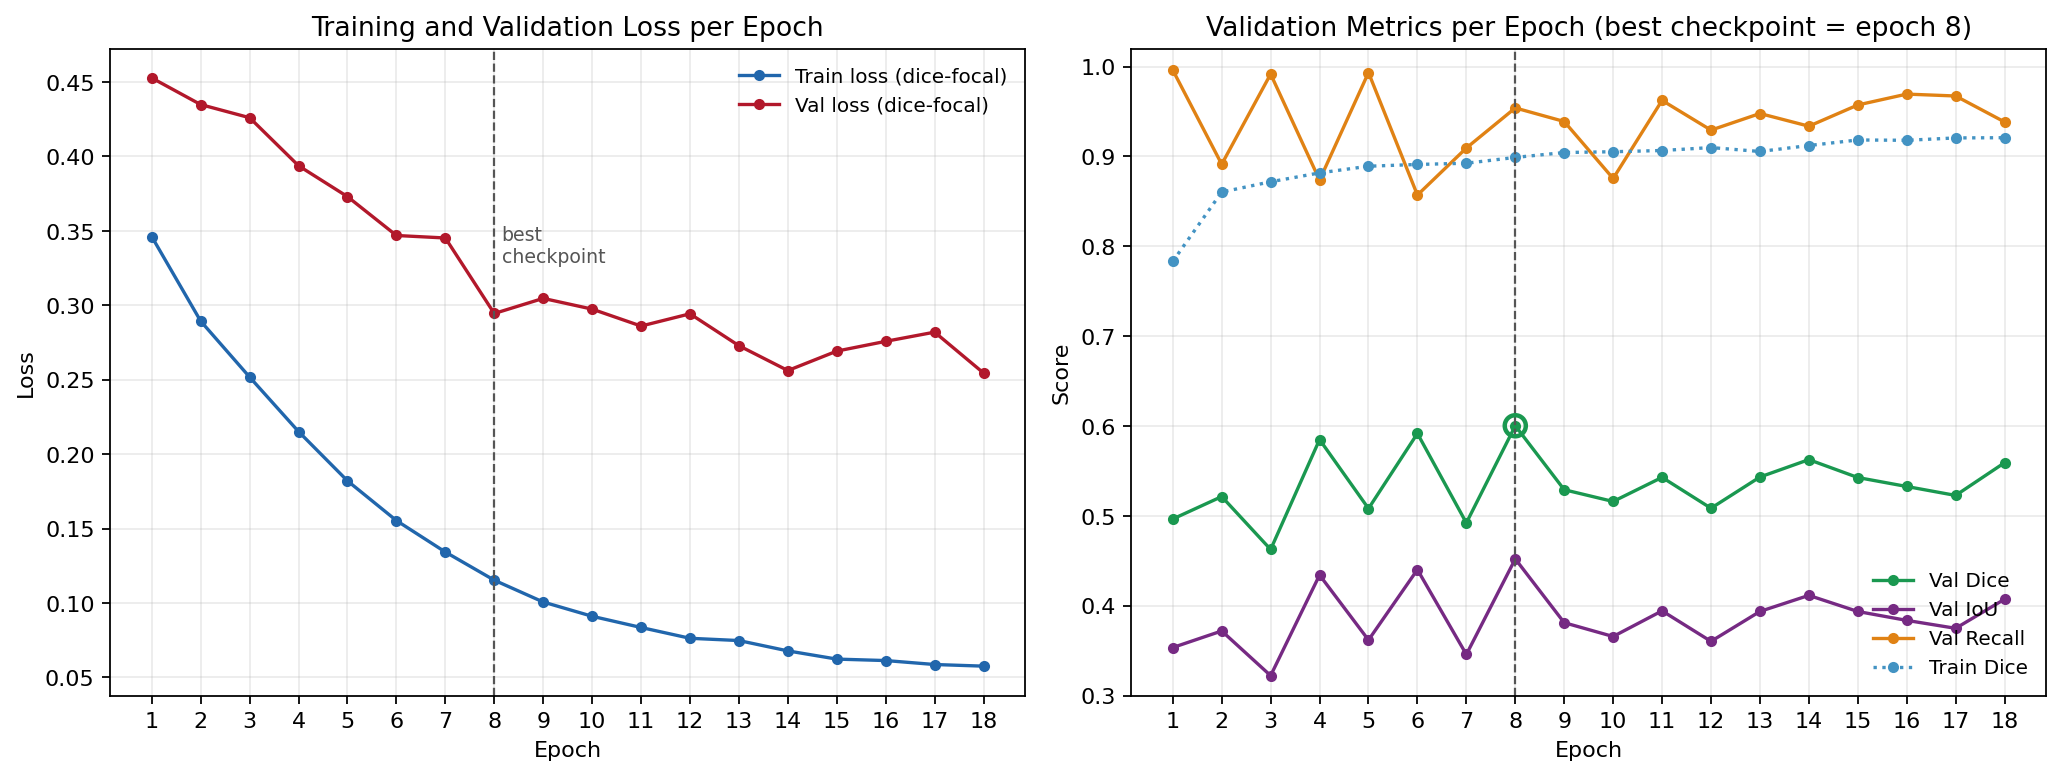
\includegraphics[width=0.95\linewidth]{training_curves_epoch_by_epoch.png}
\caption{Left: training and validation dice-focal loss per epoch. Right: validation Dice, IoU,
  recall, and training Dice per epoch. Dashed line marks epoch 8, the checkpoint selected for all
  downstream evaluation; training continued for a further 10 epochs under the patience-10
  early-stopping rule before stopping at epoch 18 without dice/IoU exceeding the epoch-8 value.}
\label{fig:training_curves}
\end{figure}

Training loss falls smoothly and monotonically across all 18 epochs (0.346 $\to$ 0.058), while
validation loss decreases far less smoothly and only until roughly epoch 8, after which it plateaus
and mildly oscillates (0.294 at epoch 8 vs.\ 0.254--0.306 for epochs 9--18), the classic
training/validation divergence pattern that early stopping is designed to catch. Validation Dice and
IoU follow the same shape: both rise unevenly through epoch 8 and then oscillate around a similar or
slightly lower level for the remaining 10 epochs (val Dice: 0.60 at epoch 8, ranging 0.51--0.59
afterward) rather than continuing to improve. Validation recall is the most volatile metric across
the whole run (oscillating between 0.857 and 0.996), consistent with a model still adjusting its
confidence threshold response on a validation set of a single volume, with only one sample in each of
the train/validation/test roles (Section~9.4), epoch-to-epoch metric swings reflect genuine sampling
variance in which patches were drawn each epoch, not measurement noise. Training Dice, by contrast,
climbs smoothly and near-monotonically throughout (0.783 $\to$ 0.921), the expected signature of a
model continuing to fit its training data after the validation metric it is being selected on has
stopped improving.

Against the thesis's stated acceptance criteria, validation recall (0.954) exceeds the 0.80 target;
validation Dice (0.600) and IoU (0.452) remain below the 0.75 and 0.60 targets respectively at the
point training was stopped.

\mysection{10.3 Held-Out Test Performance}
On the fully held-out sample\_01, the trained detector achieved Dice 0.147, IoU 0.105, precision
0.291, and recall 0.336 at the pixel level against the Bernsen pseudo-label. Considered alone, this
is a substantial drop from validation performance. However, the predicted total defect volume
fraction, 0.041\%, closely matches the pseudo-label's own volume fraction of 0.043\%
(Table~\ref{tab:podfam_classical}), while predicting fewer, larger, differently-distributed pore
instances (8,579 predicted pores vs.\ 11,928 labelled, mean diameter 6.35~px vs.\ 5.41~px). This
combination, low per-pixel overlap alongside near-identical total predicted volume, indicates the
detector has learned an approximately correct overall porosity level on data it never trained on,
while diverging from the pseudo-label's specific pore boundaries and instance count. Both the
pixel-level metrics and the volume-fraction agreement are reported together here, since either number
alone would misrepresent the result in a different direction.

\mysection{10.4 Unified Comparison}
Table~\ref{tab:podfam_unified} places the classical methods and the trained detector side by side on
the held-out test sample sample\_01.

\begin{table}[htbp]
\centering
\caption{Classical vs.\ U-Net, held-out test sample. U-Net's predicted defect fraction (0.041\%)
  sits between Otsu's near-zero result and Bernsen's label, closest to the label it was trained to
  reproduce, on data it never saw during training.}
\label{tab:podfam_unified}
\begin{tabular}{lllll}
\toprule
\textbf{Sample} & \textbf{Method} & \textbf{Defect (\%)} & \textbf{Pore count} & \textbf{Mean $\varnothing$ (px)} \\
\midrule
sample\_01 (held-out test) & Otsu             & 0.003  & 997       & 5.36 \\
                            & Yen              & 42.535 & 1,743,429 & 5.15 \\
                            & Bernsen (label)  & 0.043  & 11,928    & 5.41 \\
                            & U-Net (pred.)    & 0.041  & 8,579     & 6.35 \\
\bottomrule
\end{tabular}
\end{table}

\mysection{10.5 Extended Validation: sample\_07}
A sixth PODFAM sample, sample\_07 (1,473 slices, $1143\times1215$ pixels), was acquired and processed
after the five-sample validation reported above, using the identical preprocessing, thresholding, and
trained-detector inference pipeline described in Section~9, with no retraining or checkpoint changes.
sample\_07 was not assigned a role in the ranked train/validation/test split (Section~9.4); it is
reported here purely as an out-of-distribution check on the same epoch-8 checkpoint used throughout
Section~10.

\begin{table}[htbp]
\centering
\caption{sample\_07, full 1,473-slice volume. All three classical methods report 17--19\% defect
  fraction; the U-Net predicts 3.052\%.}
\label{tab:sample07_classical}
\begin{tabular}{llll}
\toprule
\textbf{Method} & \textbf{Defect (\%)} & \textbf{Pore count} & \textbf{Mean $\varnothing$ (px)} \\
\midrule
Otsu           & 18.177 & 330,344 & 9.15 \\
Yen            & 17.581 & 57,380  & 19.19 \\
Bernsen        & 19.369 & 354,426 & 9.15 \\
U-Net (pred.)  & 3.052  & 744,206 & 6.43 \\
\bottomrule
\end{tabular}
\end{table}

All three classical methods agree with one another on sample\_07 (17.6--19.4\%), which superficially
looks like corroboration rather than error. However, the same diagnostic applied in Section~9.5
identifies the same failure mode: sample\_07's processed slices have a mean intensity of 108.3
(measured on the mid-volume slice), below the fixed intensity threshold (128) that Bernsen's
low-contrast fallback branch uses to separate solid material from void. The auto-computed DCT for
sample\_07 (227) is, as with every other PODFAM sample, far above the approximately 15 the underlying
method reports as typical~\citep{Kim2017}, so the fallback branch dominates the classification.
sample\_05 (mean intensity 79.9, Section~9.5) showed the identical pattern at a more extreme value
and was excluded via the 10\%-defect-fraction guard; sample\_07's mean intensity is closer to the
fallback's 128 boundary, so the resulting over-estimate (17--19\%) is smaller in magnitude than
sample\_05's (approximately 52\%) but attributable to the same upstream cause.
Table~\ref{tab:sample07_diagnostic} places this in context against the four samples from
Section~10.1.

\begin{table}[htbp]
\centering
\caption{Mean processed-slice intensity vs.\ Bernsen defect fraction across all PODFAM samples. The
  two samples whose mean intensity falls below the fallback threshold (128) are exactly the two
  samples with implausibly high Bernsen defect fractions, reproducing the same failure mode at two
  different severities rather than two unrelated anomalies.}
\label{tab:sample07_diagnostic}
\begin{tabular}{lllll}
\toprule
\textbf{Sample} & \textbf{Mean intensity} & \textbf{Auto-DCT} & \textbf{Below 128?} & \textbf{Bernsen defect (\%)} \\
\midrule
sample\_01           & 167.0 & 84      & No  & 0.043 \\
sample\_02           & 142.3 & 329     & No  & 7.586 \\
sample\_04           & 163.4 & 152     & No  & 1.994 \\
sample\_07           & 108.3 & 227     & Yes & 19.369 \\
sample\_05 (excl.)   & 79.9  & 329--520 & Yes & 52.767 \\
\bottomrule
\end{tabular}
\end{table}

Under this reading, the U-Net's prediction of 3.052\% is the more credible estimate for sample\_07:
it is of the same order as sample\_02's Bernsen-labelled fraction (7.586\%) and sample\_04's U-Net
prediction (3.239\%), rather than an order of magnitude higher like the three classical methods on
this sample. This is, however, an inference-only result, sample\_07 was never assigned a
ground-truth role, so this comparison should be read as a plausibility check on the detector's
generalisation, not as a validated accuracy figure; see Section~12 for the corresponding limitation.
Figures~\ref{fig:s07_mesh}--\ref{fig:s07_mosaic} show the U-Net's predicted defect volume for
sample\_07 from four complementary viewpoints.

\begin{figure}[htbp]
\centering
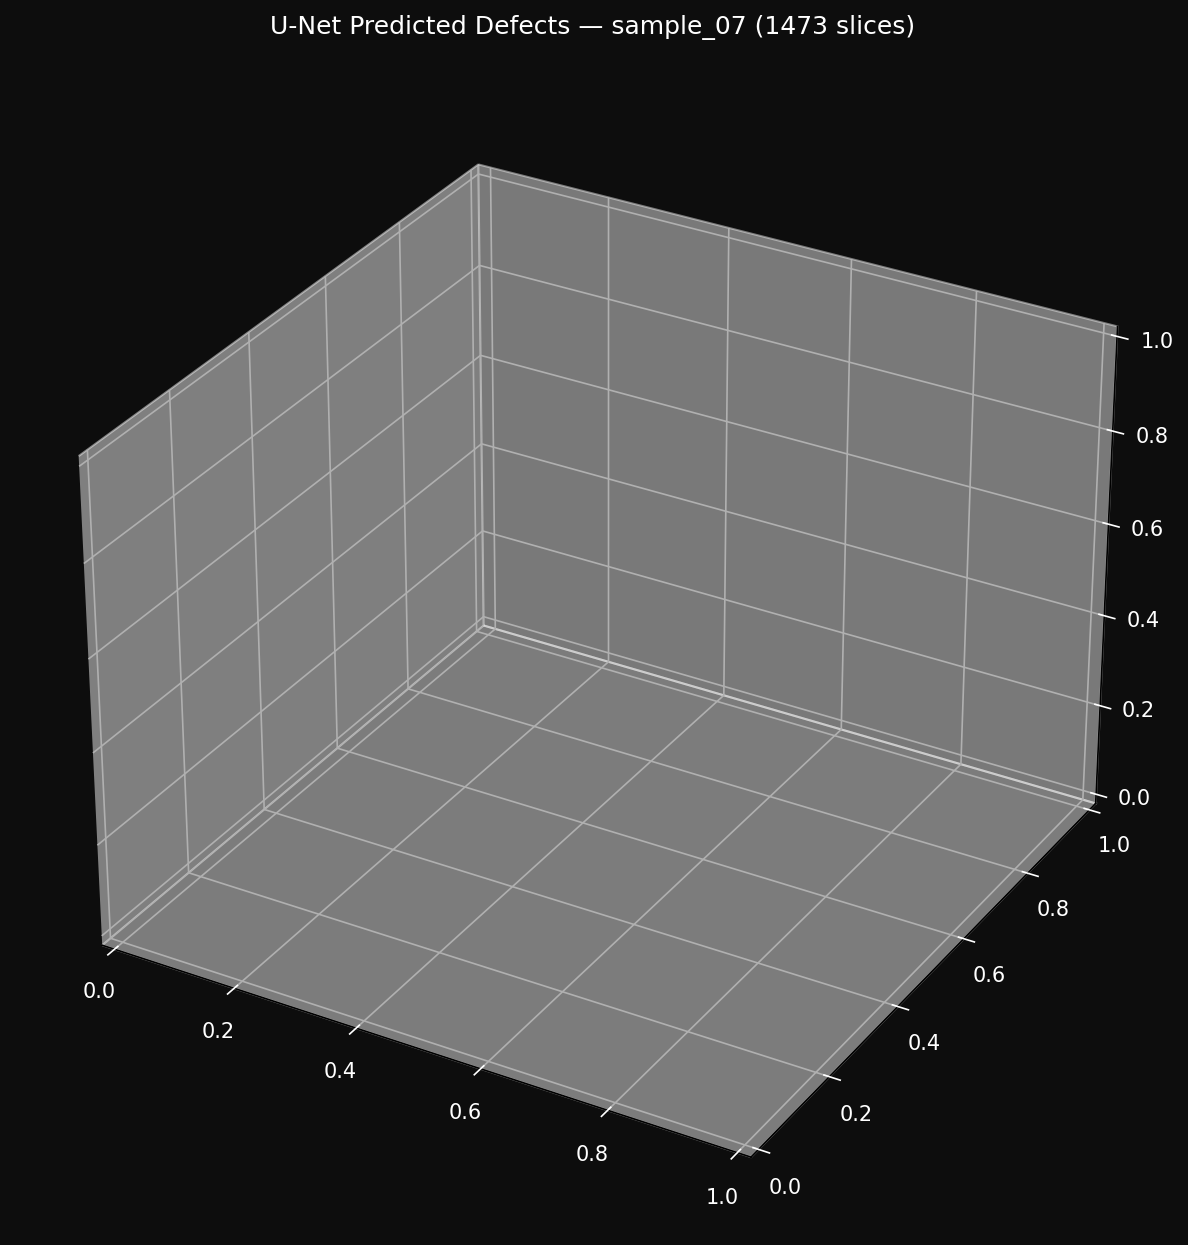
\includegraphics[width=0.75\linewidth]{sample_07_unet_3d_mesh.png}
\caption{sample\_07, U-Net-predicted defect volume, marching-cubes 3D mesh reconstruction.}
\label{fig:s07_mesh}
\end{figure}

\begin{figure}[htbp]
\centering
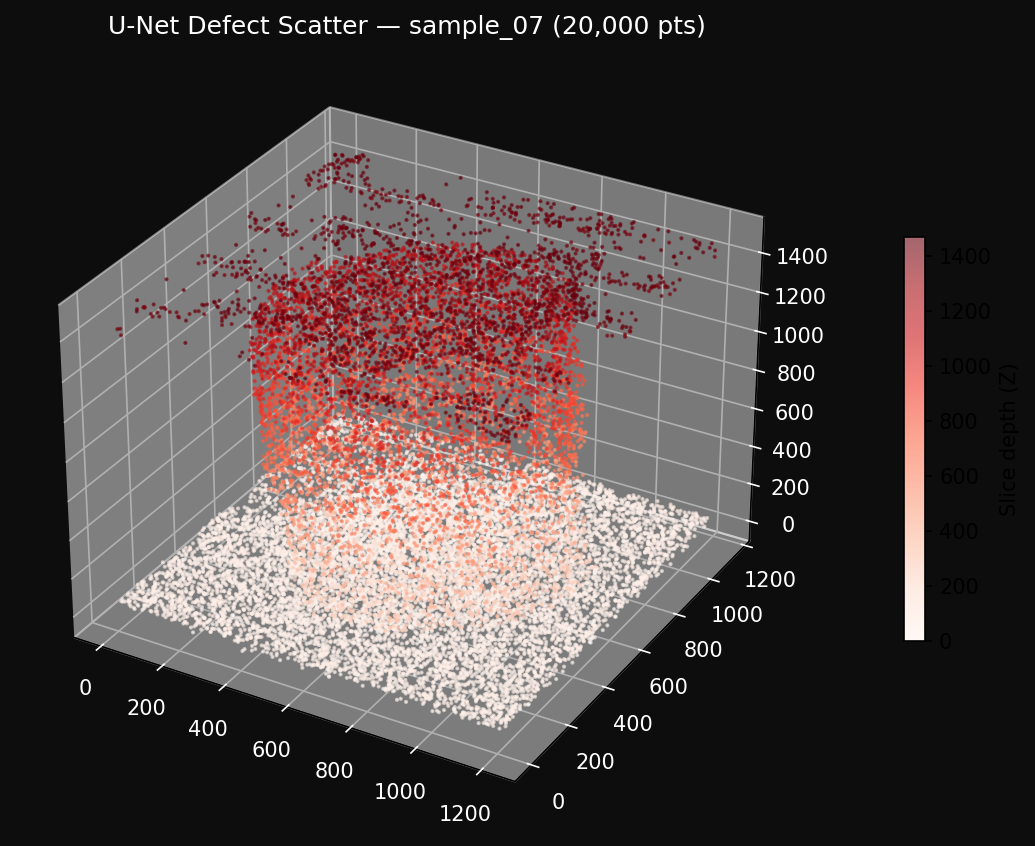
\includegraphics[width=0.75\linewidth]{sample_07_unet_defect_scatter.png}
\caption{sample\_07, U-Net-predicted defect voxel scatter, coloured by slice depth.}
\label{fig:s07_scatter}
\end{figure}

\begin{figure}[htbp]
\centering
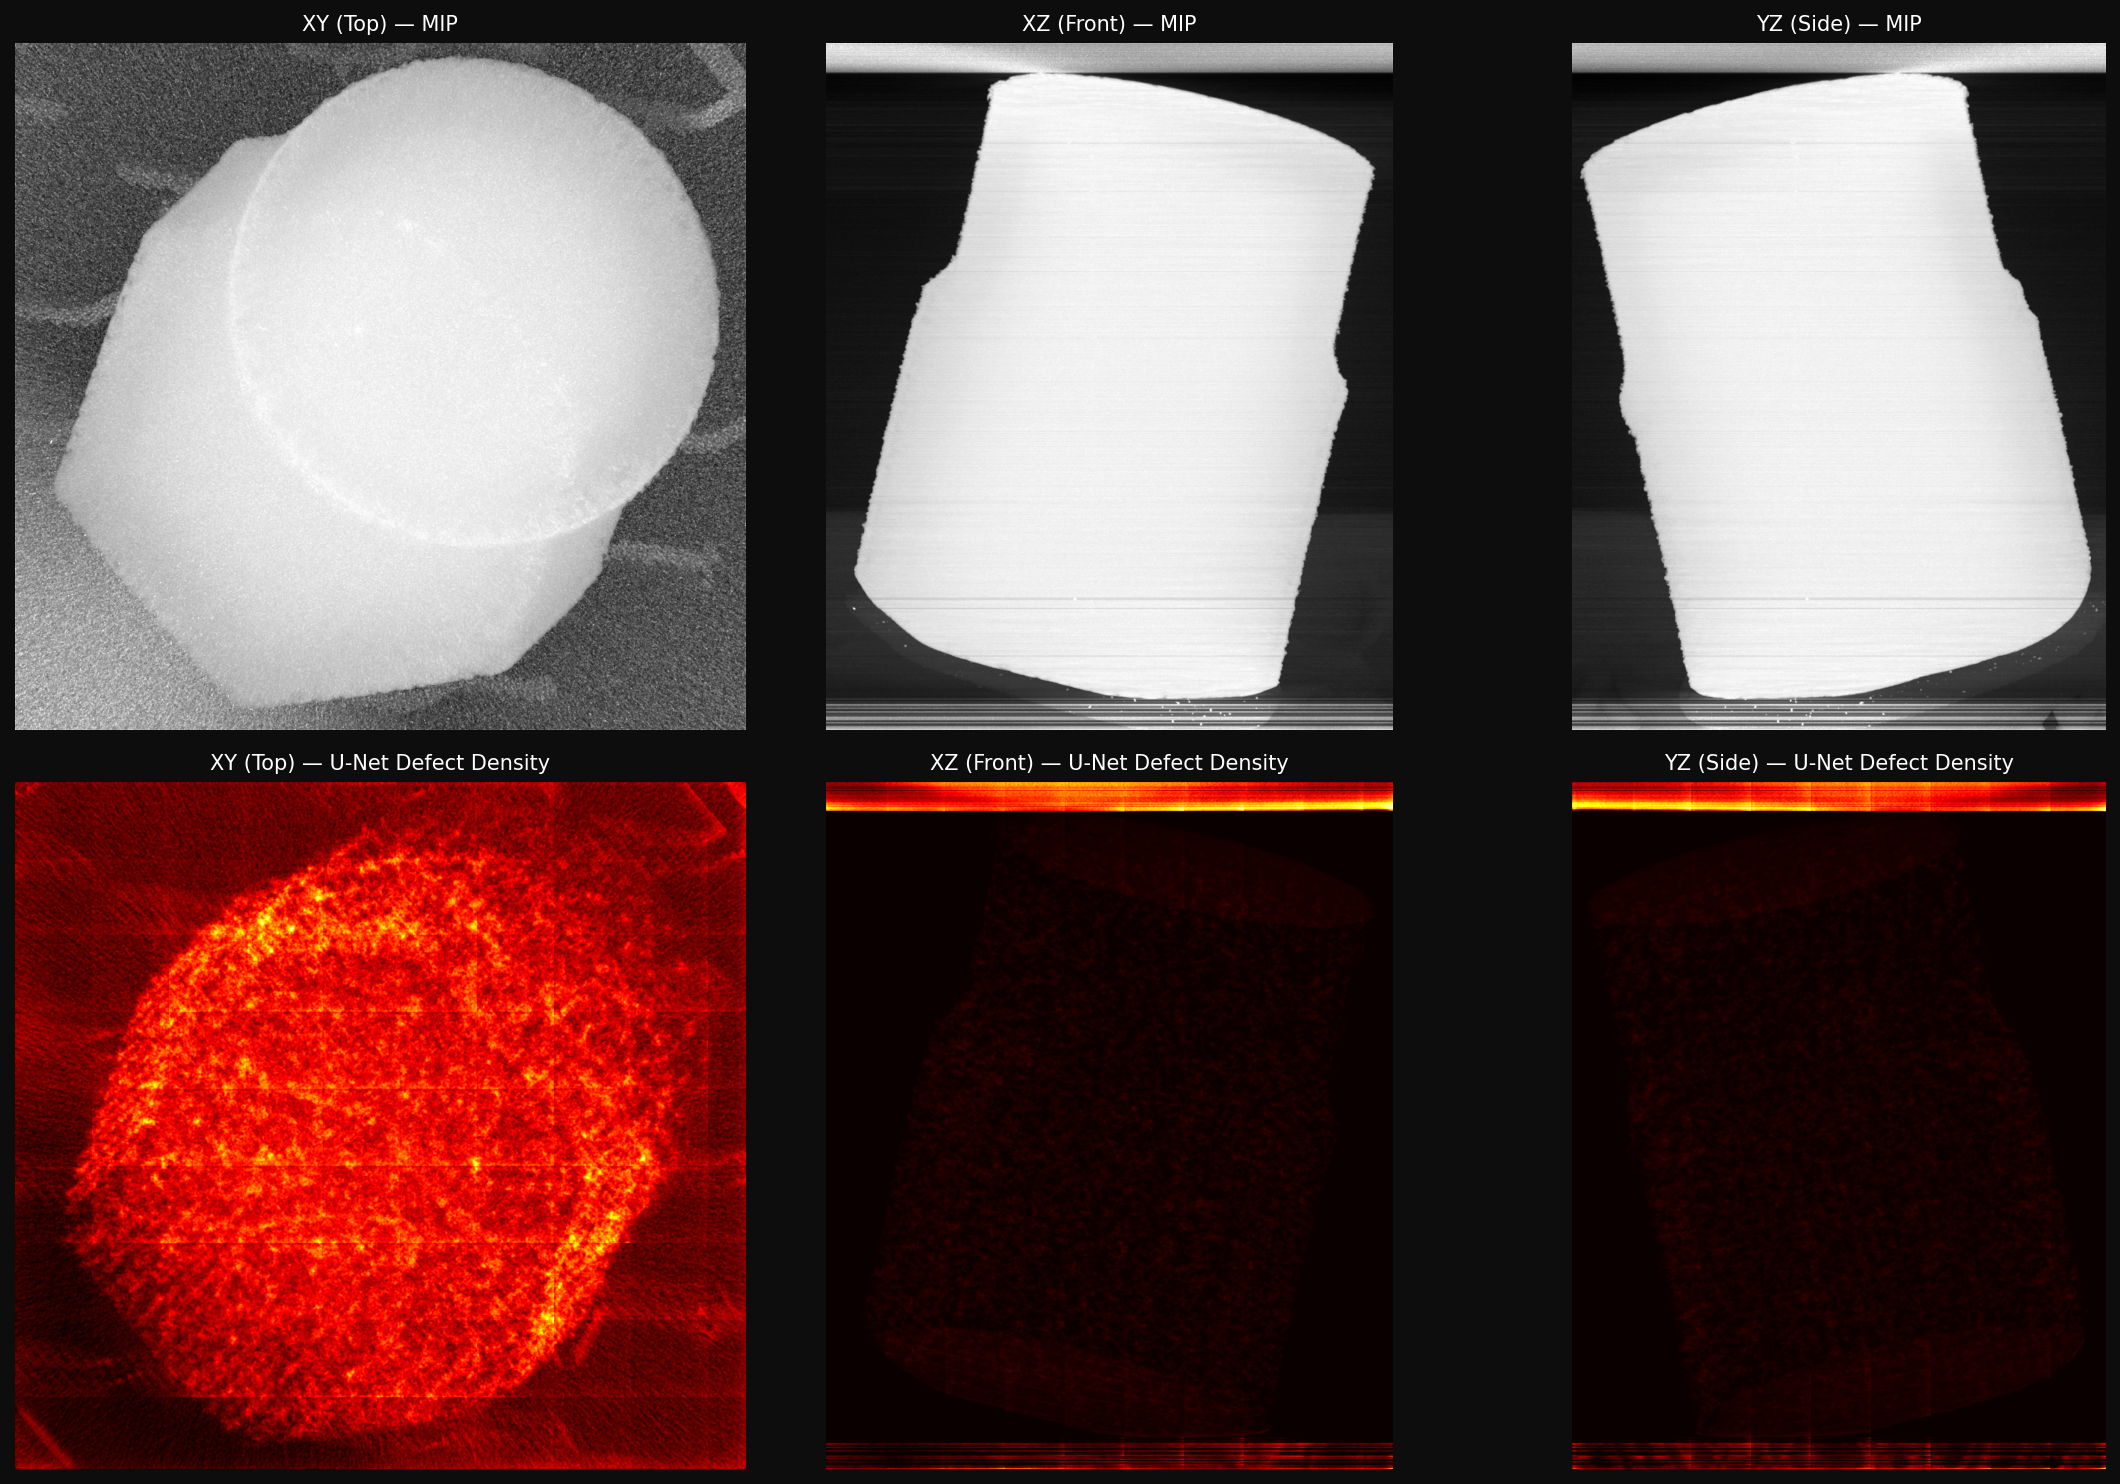
\includegraphics[width=0.95\linewidth]{sample_07_unet_orthographic_mip.png}
\caption{sample\_07, orthographic maximum-intensity projections (top row) and U-Net defect density
  projections (bottom row) along the three principal axes.}
\label{fig:s07_mip}
\end{figure}

\begin{figure}[htbp]
\centering
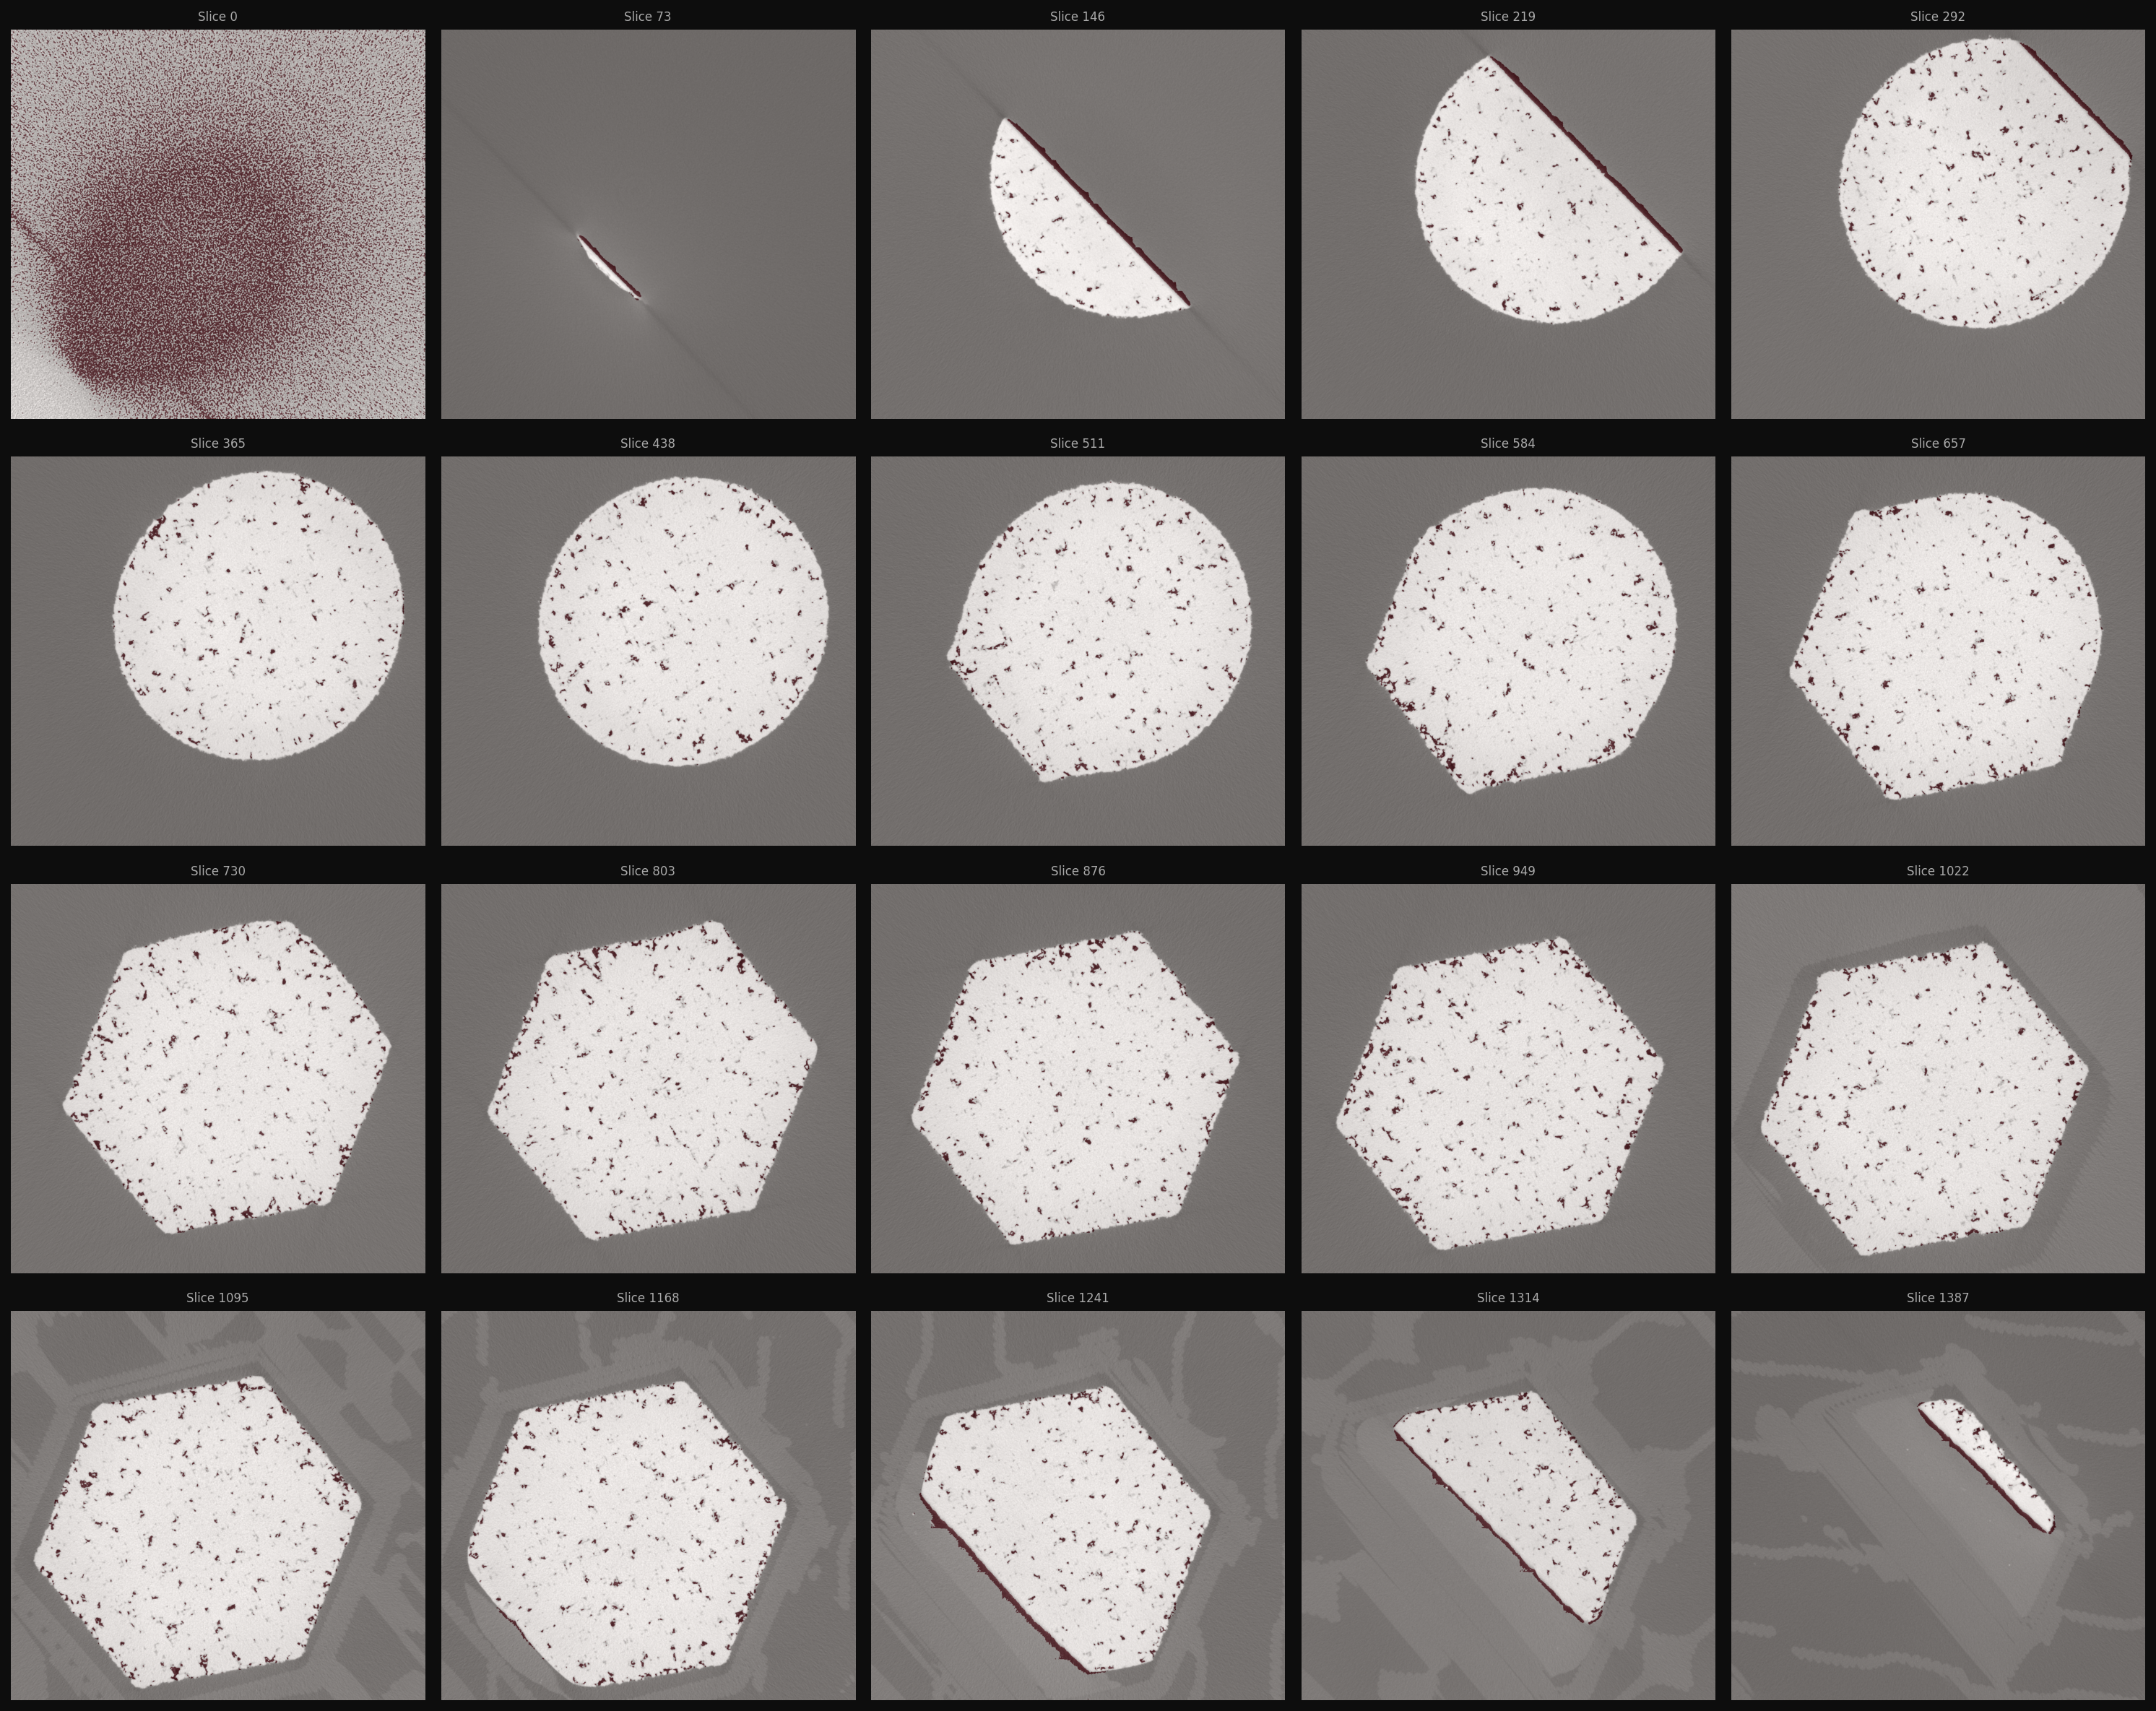
\includegraphics[width=0.95\linewidth]{sample_07_unet_slice_mosaic.png}
\caption{sample\_07, mosaic of 20 evenly-spaced slices with the U-Net's predicted defect mask
  overlaid in red.}
\label{fig:s07_mosaic}
\end{figure}

% =============================================================================
% Chapter 11: Discussion -- Part II
% =============================================================================
\mychapter{11. Discussion}

Three results from this validation phase are directly relevant to the thesis's research questions on
preprocessing, label generation, and detection performance under class imbalance.

First, the choice of pseudo-label method materially changes the reported result, not just its
magnitude. Section~8.1's literature already predicted that Bernsen would outperform Otsu and Yen on
AM XCT data~\citep{Kim2017}; this part's full-volume results confirm that prediction on an
independent dataset, and additionally show that the failure modes are not benign, Yen's
over-segmentation and Bernsen's DCT-calibration failure (Section~9.5, reproduced in Section~10.5)
each produce numbers that look superficially plausible (a percentage between 0 and 100) but are
physically wrong by one to two orders of magnitude. Any thesis reporting AM porosity from a single
thresholding method without a comparison of this kind risks reporting a number that reflects a
method's failure mode rather than the part's real condition.

Second, the sample-selection methodology (Section~9.4) is itself a result worth reporting, not only a
procedural detail. With as few as three usable samples, whichever sample is assigned to the training
role determines what the model can possibly learn; a random assignment is not a neutral default when
the sample pool is this small; a deterministic, defect-content-ranked assignment is both more
defensible and, in this case, produced a materially better and more informative result than the
random alternative.

Third, the held-out test result (Section~10.3) illustrates a general limitation of Dice/IoU as the
sole reported metric for imbalanced segmentation: on a sample with very low true defect content, a
small number of false positives can dominate the denominator and produce a low score even when the
detector's overall estimate of defect volume is accurate. Reporting the volume-fraction agreement
alongside the pixel-level metrics avoids over- or under-stating the detector's real usefulness in
either direction. The sample\_07 extension (Section~10.5) reinforces this point from a different
angle: three independent classical methods agreeing with each other (17.6--19.4\%) was not, on
inspection, corroboration of a real result, it was three methods sharing the same upstream
sensitivity to processed-image mean intensity.

% =============================================================================
% Chapter 12: Limitations -- Part II
% =============================================================================
\mychapter{12. Limitations}

\begin{itemize}
\item No independently verified ground truth exists for any PODFAM sample. Every Dice, IoU,
  precision, and recall value in this part measures agreement with the Bernsen pseudo-label, not
  with a verified physical defect map. Bernsen was selected because comparative literature reports
  it as the more reliable of the three classical methods evaluated~\citep{Kim2017}, but it remains a
  proxy rather than ground truth.
\item The core validation set comprises five samples, two of which were excluded (sample\_03 as
  near-empty, sample\_05 for a documented labelling artefact), leaving a 1-train / 1-validation /
  1-test split. This sample size cannot support a statistical claim of generalisation; the reported
  results should be read as a feasibility demonstration on this pipeline and this specific data, not
  as an estimate of expected performance on unseen PODFAM parts in general.
\item Training uses 80 evenly-spaced slices per volume rather than the full 749--900, a deliberate
  trade-off to keep per-epoch training time practical on the available hardware; full-slice training
  was measured to exceed three hours per epoch under equivalent conditions.
\item The pixel-to-physical-unit conversion factor (\texttt{PIXEL\_SIZE\_UM}) used elsewhere in this
  pipeline's configuration was not calibrated to the PODFAM scans' actual voxel size for this
  validation phase; all size figures in this part are reported in pixels, not micrometres, for that
  reason.
\item Preprocessing for the PODFAM phase (Section~9.2) omits the beam-hardening correction and
  ring-artefact suppression stages used in the Part I pipeline; the two parts' preprocessing outputs
  are not numerically comparable to one another.
\item sample\_07 (Section~10.5) is a single additional sample run through inference only, with no
  ground-truth role and no retraining. Its U-Net prediction being more plausible than the classical
  methods' is a single data point consistent with the pipeline's other results, not an independent
  validation of detector accuracy on new, unseen scan conditions.
\end{itemize}

% =============================================================================
% Chapter 13: Conclusion -- Part II
% =============================================================================
\mychapter{13. Conclusion}

This part validated the thesis's automated XCT defect-detection pipeline on real PODFAM metal AM
samples, independently of the NIST CoCr benchmark used in Part I. Full-volume comparison confirmed,
on new data, the literature's finding that Bernsen local thresholding outperforms Otsu and Yen for AM
porosity segmentation, and additionally surfaced and diagnosed a specific calibration failure mode in
Bernsen's automatic contrast-threshold estimation, a failure mode subsequently reproduced, at a
different severity, on a sixth sample processed after the original validation. A 2D U-Net trained on
Bernsen pseudo-labels, using a defect-content-ranked rather than random sample assignment, achieved a
best validation Dice of 0.600 and, on a fully held-out sample, predicted a total defect volume within
0.002 percentage points of the pseudo-label's own value, a result that argues for reporting
volume-level agreement alongside pixel-level overlap metrics in future evaluation of this pipeline.
The validation set's small size and the absence of independently verified ground truth are stated
explicitly as limits on how far these results can be generalised, consistent with the standard set in
Part I's own treatment of its NIST-phase pseudo-labels.

Taken together with Part I, this document now covers method development on a public benchmark (NIST
CoCr), full-volume classical-vs-deep-learning validation on real industrial process-monitoring data
(PODFAM, five core samples), and an out-of-distribution generalisation check on a sixth sample that
both supported the trained detector's usefulness and surfaced a reproducible, previously undocumented
failure mode in one of its classical comparison baselines.


% ---------------------------------------------------------------------------
% PART III -- Extended validation: loss-function, preprocessing, and
% boundary-detection ablations; conv-block attribution; strengthened
% external validation
% ---------------------------------------------------------------------------
\clearpage
\begin{center}
{\large\bfseries PART III}\\[4pt]
{\Huge\bfseries EXTENDED VALIDATION}\\[8pt]
{\large\itshape Loss-Function, Preprocessing, and Boundary-Detection Ablations on the\\
PODFAM Pipeline, with Network Attribution and Strengthened External Validation}
\end{center}
\clearpage

% =============================================================================
% Chapter 14: Method -- Part III (Extended Validation)
% =============================================================================
\mysection{Note on scope (Part III)}
This part reports a later phase of work, conducted after the five/seven-sample PODFAM validation of
Part II, that revisits several of that validation's design choices under controlled ablation: which
loss function the detector is trained with, whether beam-hardening and ring-artefact correction help
on PODFAM data as they did in Part I, whether the circular sample-boundary assumption can be safely
replaced for non-circular parts, and what a genuinely held-out sample reveals about the detector's
real generalisation. It also reports two analyses not tied to any single ablation: a gradient-based
interpretability study of the trained detector, and a strengthening of the pipeline's external
validation against independently published reference porosity. Every figure and table in this part
was generated directly from the working pipeline during this phase; none of Part I's or Part II's own
figures or numbers were re-run, re-verified, or altered here. Where this part's methodology differs
materially from Part II, most importantly, the train/validation/test sample assignment described in
Section~14.3 below, the difference is stated explicitly rather than silently merged with the Part II
description.

\mychapter{14. Method --- Extended Validation}

\mysection{14.1 Scope and Relationship to Parts I and II}
Three questions motivate this part, each building on a specific claim made without controlled
comparison earlier in the thesis. First, Part II's detector (Section~9.6) used the combined Dice-Focal
loss without comparing it against the alternatives Part I's Section~3.8 lists; Section~14.3 below
reports a controlled four-way comparison on PODFAM data. Second, Part I's preprocessing pipeline
(Section~3.3) includes beam-hardening correction (BHC) and ring-artefact suppression, but Part II's
preprocessing (Section~9.2) omits both; Section~14.4 tests whether adding them to the PODFAM pipeline
changes detector performance. Third, Part II's sample-boundary detection (Section~9.3) fits a single
circular mask per volume, an assumption later found not to hold for two PODFAM samples
(sample\_06/07) with non-circular, part-specific cross-sections; Section~14.5 replaces it with a
shape-agnostic method for those samples specifically. A fourth strand, reported in
Sections~14.8--14.10, is not an ablation of an earlier choice but new analysis: which parts of the
trained network drive its output, and how strong is the thesis's external validation once the
reference porosity source's own experimental grounding is checked.

\mysection{14.2 Sample Set: Geometric Diversity and the Waygate Scanner}
All PODFAM samples (Section~9.1) are Ti-6Al-4V, manufactured by laser powder bed fusion on an Aconity
Two machine and scanned on a Waygate v\textbar tome\textbar x M~240 XCT system. The seven-sample set
spans a deliberately varied range of cross-sectional geometry, from the circular cross-sections of
sample\_01--05 to the hexagonal and other non-circular cross-sections of sample\_06 and sample\_07,
included specifically to test the pipeline beyond a single clean cylindrical benchmark. This geometric
diversity is the direct motivation for Section~14.5: a boundary-detection method that assumes a
circular cross-section, adequate for sample\_01--05, systematically misdetects the true material
boundary on sample\_06/07, either clipping real material at the corners of the hexagonal section or
extending the mask past the true boundary into background, which is then misread as defect.

\mysection{14.3 Loss-Function Ablation}
Four loss-function configurations, binary cross-entropy (BCE), Dice, Focal, and combined Dice-Focal
(the formulation used throughout Part II), are trained and compared under an otherwise identical
configuration, isolating loss function as the only varying factor. \texttt{config.py}'s
\param{TRAINING\_SAMPLES\_OVERRIDE} is pinned to the same four-sample list,
\texttt{["sample\_02", "sample\_04", "sample\_03", "sample\_01"]}, most-voids-first, for every run.
\texttt{pipeline.py}'s \texttt{split\_volumes()} assigns roles by rank position rather than by patch,
the first \param{n\_train} names become training samples, the next \param{n\_val} become the single
validation sample, and the remainder become the single held-out test sample, so with four samples and
the pipeline's default 20\%/10\% val/test split this resolves to \textbf{sample\_02 and sample\_04
pooled for training, sample\_03 for validation, and sample\_01 held out entirely for testing}. This is
a whole-sample split, not a patch-level split within a shared pool: sample\_01, the same sample used
as the held-out test role throughout Part II (Section~9.4), never contributes any patch to training
or validation in any of the four runs. sample\_03, excluded from training in Part II as near-empty
(Section~9.4), is used here in the validation role, since a near-empty sample is unsuitable for
training but still usable to monitor convergence. All four runs otherwise use the training
configuration of Section~9.6 unchanged: $256\times256$ patches with 50\% overlap, stratified 1:3
foreground-to-background sampling, Adam optimisation at learning rate $4\times10^{-5}$, up to 50
epochs with early stopping (patience 10 epochs), and best-checkpoint selection by validation Dice.
Every run's total epoch count equals its best epoch plus exactly 10, confirming early stopping, rather
than the 50-epoch cap, was the actual stopping condition in all four cases.

\mysection{14.4 Preprocessing Ablation}
The best-performing configuration from Section~14.3 is retrained with the four-stage Part I
preprocessing pipeline (percentile normalisation, BHC, ring-artefact suppression, NLM denoising,
Section~3.3) applied to the PODFAM volumes in place of Part II's narrower three-stage pipeline
(Section~9.2), using the identical sample split described above. This isolates the marginal effect of
BHC and ring suppression on PODFAM data specifically, since Part I's own parameter sensitivity
analysis (Section~3.3.6) was conducted only on the NIST CoCr dataset and its conclusions were never
previously tested on PODFAM's different scanner and material.

\mysection{14.5 Shape-Aware Sample-Boundary Detection}
For sample\_06 and sample\_07, the circular-fit boundary method (Section~9.3) is replaced with a
sliding-window boundary scan that locates the sample surface by its local intensity peak along each
scan line, without assuming any particular cross-sectional shape, followed by taking the largest
connected component of the resulting interior region and eroding it by a fixed margin
(\param{erosion\_radius} = 35~px) to exclude partial-volume edge pixels. The erosion margin was
selected by a parameter sweep (25, 30, 35, and 40~px), the false boundary artefact it is designed to
remove shrinks smoothly and predictably as the margin increases across this range, and 35~px was the
value visually verified to fully remove the artefact, described in Section~15.3, without eroding
genuine material at the sample interior. A hybrid fallback is required for a minority of slices near
the top and bottom of a volume, where support-structure content rather than open air surrounds the
part: on these transition slices, the primary fixed-threshold detector can fail to find any background
at all (an apparent mask coverage near 100\%), triggering a per-slice adaptive-Otsu re-estimate for
that slice only. This fallback is not fully closed as an edge case, see Section~17 for the specific
failure mode it can itself produce on very high-porosity content. For sample\_01--05, the original
circular-fit method (Section~9.3) is retained unchanged, since it already performs correctly on these
genuinely circular samples; sample\_05 specifically requires a fixed intensity threshold rather than
adaptive Otsu for its own boundary fit, because its unusually high porosity (Section~9.5,
Table~\ref{tab:podfam_classical}) leaves too few solid-material pixels for Otsu's two-class assumption
to separate correctly, a sample-content-dependent choice rather than a universal preference for one
threshold strategy over the other.

\mysection{14.6 A Documented Negative Result: Canny Edge Detection}
Canny edge detection with morphological closing was investigated as a further alternative to both the
circular-fit and shape-aware boundary methods, restricted to boundary detection only (it was not
carried forward into any trained-model comparison). On sample\_01--05, its results closely reproduce
the production circular-fit numbers (Section~15.3), confirming those results independently rather than
replacing them. On sample\_06/07, it exhibits a specific and confirmed failure mode on a small number
of slices: rather than following the true material boundary, it confidently traces the edge of the
surrounding support scaffold instead, producing a boundary that looks well-formed rather than an
obvious error. Investigation traced this to the underlying image signal itself: at the specific slices
where the failure occurs, the material-to-background intensity contrast has genuinely faded to
approximately the same strength as the scaffold's own edge contrast, so no threshold, smoothing
parameter, or shape heuristic (solidity, area continuity, and brightness were each tried as
tie-breakers) can reliably distinguish the two closed shapes from the image content alone. This is
reported as a negative result specifically because the cause is a property of the data at those depths
rather than a fixable implementation choice; the shape-aware method of Section~14.5 remains the
production method for sample\_06/07 for this reason.

\mysection{14.7 Background-Masking Correction for Detector Inference}
A separate defect, found by inspecting the trained detector's predictions on sample\_07 (an
out-of-distribution inference check, not part of the training or validation roles of
Section~14.3), was that the network produced implausible defect predictions on slices with little or
no metal in frame, near-empty transition and support-structure slices the training data never
specifically taught it to recognise as background. The fix applies the same shape-aware boundary
detector used in Section~14.5 to zero out background both before the trained network sees a slice and
again on its predicted output, rather than relying on the network to infer the sample boundary
implicitly from intensity alone.

\mysection{14.8 Conv-Block Attribution Analysis}
To identify which stages of the trained 2D U-Net (architecture per Section~3.7.1, verified by direct
instantiation to have exactly 31,037,633 trainable parameters) contribute most to the defect decision,
a forward hook is registered on every convolutional block's output (four encoder blocks, the
bottleneck, and four decoder blocks, nine blocks total), and \texttt{retain\_grad()} is called on each
hooked output. A forward and backward pass is run on a representative $256\times256$ crop from
sample\_02 (14.27\% genuine Bernsen-labelled defect content), with the scalar objective
$\sum(\hat{y} \odot y)$, the predicted defect probability map $\hat{y}$ elementwise-multiplied by the
Bernsen ground-truth mask $y$ and summed, backpropagated to populate every hooked block's gradient.
Each block's relative contribution is then computed as the mean absolute value of activation times
gradient, $\overline{|a \cdot \nabla a|}$, at that block, normalised across all nine blocks to sum to
100\%. This is a single representative crop and a single attribution method, gradient$\times$activation
is a simple, interpretable choice but not the only one available, so the result reported in
Section~15.6 is directional evidence about where the network's decision-relevant signal concentrates,
not an exhaustive architectural study. The analysis is run on the checkpoint identified in
Section~14.3 as the strongest of the four loss-function configurations (BCE), verified to be the
correct checkpoint by an exact match between its own recorded validation Dice and best epoch
(0.7275 at epoch 13) and the same figures reported independently for the loss-ablation's BCE run.

\mysection{14.9 External Validation Against Independently Published Porosity}
Otsu, Yen, and Bernsen thresholding are each compared, per NIST CoCr sample, against the porosity
values independently published by Kim et al.~\citep{Kim2017} for the same physical samples, using the
Pearson correlation coefficient $r$ across the five samples in common. This validates the classical
methods against a source external to this pipeline, rather than against another output of the same
pipeline. A further check was made of Kim et al.'s own reference values themselves: their paper
reports cross-validating their XCT-derived porosity against an independent gravimetric (density-based)
method, computed from measured disk mass and cobalt-chrome's nominal density, for several of their
samples, with the two methods agreeing to within 1--4\% absolute and an XCT-side threshold-sensitivity
uncertainty below $\pm 0.12\%$~\citep{Kim2017}. This means the reference this thesis's own $r$ value is
measured against is not itself only another XCT measurement, it carries independent physical grounding
one step back. This gravimetric cross-check in Kim et al.'s own paper was reported for specific samples
(their own sample numbering 2, 4, 5, and 6); it has not been independently confirmed here that every
one of the five NIST samples used in this thesis's correlation individually received that exact check,
as opposed to being reported as part of their broader dataset characterisation, and this caveat is
carried into the results and limitations of this part accordingly.

\mysection{14.10 Physical Voxel-Size Determination}
\texttt{config.py}'s \param{PIXEL\_SIZE\_UM} constant, which converts pixel-based measurements
elsewhere in this pipeline to physical units, was never calibrated to either dataset's actual scan
resolution and remains at its unfilled placeholder value of 1.0 (Section~12); this part reports the
actual physical scale for both datasets as a measurement, without editing that constant in the running
pipeline. For PODFAM, the raw TIFF files for sample\_06 and sample\_07 carry embedded
\texttt{XResolution}/\texttt{YResolution} metadata tags, read directly from the file headers, giving a
consistent voxel size of 12.001~\textmu m/px for both samples. For the NIST CoCr samples, the raw TIFF
files carry no equivalent spatial metadata (only an ImageJ-style intensity min/max in each file's
\texttt{ImageDescription} field), so the voxel size is instead taken from the dataset's own published
documentation~\citep{NIST_CoCr}, which states a nominal voxel size of approximately 2.5~\textmu m for
most samples in the set, with samples 3 and 5 specifically scanned at a substantially finer 0.87~\textmu
m. This roughly threefold difference in resolution for exactly the two samples this thesis already
excludes from training, sample\_03 as near-empty and sample\_05 for the DCT labelling artefact
(Sections~9.4, 9.5), is noted in Section~16 as a plausible, previously unidentified explanation worth
stating explicitly, a finer voxel size implies a smaller physical field of view per slice for the same
pixel dimensions, which could plausibly affect both the amount of defect content captured and the
image's intensity/contrast profile. This is reported here as a hypothesis consistent with the
available evidence, not as a confirmed causal finding; it has not been independently tested against
the two samples' actual field-of-view dimensions or intensity statistics within this work.

% =============================================================================
% Chapter 15: Results -- Part III (Extended Validation)
% =============================================================================
\mychapter{15. Results --- Extended Validation}

\mysection{15.1 Loss-Function Ablation Results}
Table~\ref{tab:loss_ablation} reports validation-set performance for all four loss configurations,
trained and evaluated under the identical split described in Section~14.3.

\begin{table}[htbp]
\centering
\caption{Loss-function ablation, validation-sample (sample\_03) results. BCE achieves the best raw
  Dice and IoU of the four configurations.}
\label{tab:loss_ablation}
\begin{tabular}{lllll}
\toprule
\textbf{Loss} & \textbf{Val Dice} & \textbf{Val IoU} & \textbf{Precision} & \textbf{Recall} \\
\midrule
BCE                    & \textbf{0.7275} & \textbf{0.6235} & 0.809 & 0.7206 \\
Dice                   & 0.691           & 0.578           & 0.822 & 0.672 \\
Combined Dice-Focal (Part II's choice) & 0.696 & 0.578      & 0.741 & 0.7278 \\
Focal                  & 0.574           & 0.466           & \textbf{0.976} & 0.471 \\
\bottomrule
\end{tabular}
\end{table}

BCE achieves the best Dice and IoU of the four configurations. It was not selected as the primary
formulation when this comparison was first run, combined Dice-Focal was retained instead on the
grounds of a more balanced precision/recall trade-off, but re-examining the exact figures shows that
framing overstated the difference: BCE's recall (0.7206) is only 0.0072 below combined Dice-Focal's
(0.7278), not a meaningful trade-off given the other three metrics all favour BCE outright. Separately,
and independently of this ablation, the held-out generalisation-gap checkpoint identified in
Section~15.2 below records a validation Dice of 0.7275 at epoch 13, an exact match to this table's BCE
row, confirming that checkpoint was already trained with BCE loss. Taken together, these two points of
evidence support formalising BCE as the primary loss function for this pipeline going forward, rather
than combined Dice-Focal.

\mysection{15.2 The Generalisation Gap}
Table~\ref{tab:generalisation_gap} reports the same checkpoints' Dice on their validation sample
(sample\_03) against their Dice on the fully held-out test sample (sample\_01, never included in
training or validation for any configuration in this part).

\begin{table}[htbp]
\centering
\caption{Validation Dice vs.\ held-out test Dice, across the preprocessing and masking ablations of
  Sections~14.3--14.5. All configurations share the same held-out sample, sample\_01. Acceptance
  criteria (Dice~$\geq$~0.75, IoU~$\geq$~0.60, Recall~$\geq$~0.80) fail in every configuration on the
  held-out sample.}
\label{tab:generalisation_gap}
\small
\begin{tabular}{p{7.8cm}p{3.2cm}p{3.2cm}}
\toprule
\textbf{Configuration} & \textbf{Validation Dice} & \textbf{Held-out test Dice} \\
\midrule
BCE, baseline (3-stage) preprocessing, circular mask & 0.7275 & 0.1218 \\
BCE, + BHC/ring preprocessing, circular mask         & 0.7013 & 0.1693 \\
BCE, + BHC/ring preprocessing, shape-aware mask       & $\sim$0.70 & 0.2119 \\
\bottomrule
\end{tabular}
\end{table}

Every configuration shows the same pattern: validation Dice in the 0.70--0.73 range, held-out test
Dice far lower, 0.12--0.21. This gap is present in the original (Part II) configuration as well
(Section~10.3: validation Dice 0.600, held-out test Dice 0.147), so it is corroborated by two
independently run experiments using different sample-role assignments and different loss/preprocessing
configurations, not an artefact of one specific run. Table~\ref{tab:preproc_ablation} reports the full
held-out test metrics for the two directly comparable configurations (baseline vs.\ BHC/ring,
circular mask both).

\begin{table}[htbp]
\centering
\caption{Preprocessing ablation, full held-out test set metrics (sample\_01), circular mask both
  configurations.}
\label{tab:preproc_ablation}
\begin{tabular}{lllll}
\toprule
\textbf{Configuration} & \textbf{Dice} & \textbf{IoU} & \textbf{Precision} & \textbf{Recall} \\
\midrule
Baseline (3-stage preprocessing) & 0.1218 & 0.0907 & 0.2908 & 0.3134 \\
+ BHC and ring-artefact correction & 0.1693 & 0.1328 & 0.4049 & 0.2974 \\
\bottomrule
\end{tabular}
\end{table}

Held-out test Dice improves by 39\% relative (0.1218 $\to$ 0.1693) with BHC/ring correction added,
while validation Dice moves slightly in the opposite direction (0.7275 $\to$ 0.7013). Read together,
this indicates the preprocessing change improves genuine generalisation to unseen data rather than
fitting the validation sample more closely, since the more trustworthy of the two numbers (held-out,
never used for any training decision) improved while the less trustworthy one (validation, used for
checkpoint selection) did not. Adding the shape-aware boundary mask of Section~14.5 on top of BHC/ring
continues the same trend, held-out Dice rises further to 0.2119, a monotonic improvement across all
three configurations (0.1218 $\to$ 0.1693 $\to$ 0.2119) even though every configuration still fails the
thesis's acceptance criteria by a wide margin.

\mysection{15.3 Shape-Aware Masking Results}
Table~\ref{tab:podfam_shape_aware} reports the corrected full-volume Bernsen defect statistics for
sample\_06 and sample\_07 using the shape-aware boundary method of Section~14.5, alongside the
uncorrected result the original erosion setting produced.

\begin{table}[htbp]
\centering
\caption{sample\_06/07, shape-aware boundary detection, before and after erosion-margin correction.
  sample\_06's initial result was found to be a boundary artefact, not genuine porosity; sample\_07's
  corrected result was confirmed genuine by visual inspection of the full slice mosaic.}
\label{tab:podfam_shape_aware}
\small
\begin{tabular}{p{2.2cm}p{6.5cm}p{5.5cm}}
\toprule
\textbf{Sample} & \textbf{Defect fraction, erosion=8px (uncorrected)} & \textbf{Defect fraction, erosion=35px (corrected)} \\
\midrule
sample\_06 & 2.92\% (boundary rim artefact) & \textbf{0.030\%} \\
sample\_07 & --- & \textbf{0.759\%} \\
\bottomrule
\end{tabular}
\end{table}

sample\_06's uncorrected result (2.92\%) is roughly two orders of magnitude above its corrected value
(0.030\%), traced to a thin rim of partial-volume boundary pixels being misclassified as defect at the
original 8~px erosion margin; a sweep of erosion values (25, 30, 35, and 40~px) showed the false rim
shrinking smoothly and predictably as the margin increased, with 35~px selected as the value fully
removing the artefact without eroding genuine interior material. sample\_07's corrected result
(0.759\%) was cross-checked by direct visual inspection of its full slice mosaic and judged to reflect
genuine porosity rather than a residual boundary effect. For comparison, the circular-fit method
applied to sample\_01--05 in this same later pipeline pass gives full-volume Bernsen defect fractions
of 0.055\% (sample\_01), 6.494\% (sample\_02), 0.181\% (sample\_03), 1.641\% (sample\_04, adaptive
Otsu boundary threshold), and 53.42\% (sample\_05, fixed boundary threshold, required because its
$\sim$72\% porosity leaves too few solid pixels for Otsu's two-class assumption to hold, Section~14.5).
These figures are from an independently re-run pipeline pass and are not identical to Section~10.1's
Table~\ref{tab:podfam_classical} figures for the same samples, both are genuine pipeline outputs from
different points in this work and are reported here as such rather than reconciled into one number.

The Pearson correlation between each classical method's per-sample defect fraction and Kim et
al.'s~\citep{Kim2017} independently published porosity (Section~14.9, five NIST samples in common)
was recomputed under the circular, no-mask, and shape-aware boundary configurations, to check whether
replacing the circular assumption changes the pipeline's already-established external-validation
accuracy. Table~\ref{tab:mask_r_comparison} shows the result.

\begin{table}[htbp]
\centering
\caption{Pearson $r$ vs.\ Kim et al.'s published porosity, by boundary-detection method (NIST samples,
  $n=5$). Removing the boundary mask entirely is unusable; shape-aware masking is statistically
  indistinguishable from the circular mask it replaces.}
\label{tab:mask_r_comparison}
\begin{tabular}{llll}
\toprule
\textbf{Method} & \textbf{Circular mask} & \textbf{No mask} & \textbf{Shape-aware mask} \\
\midrule
Otsu    & 0.983 & 0.984 & 0.982 \\
Yen     & 0.503 & $\sim$0.43 & $\sim$0.50 \\
Bernsen & \textbf{0.995} & 0.992 & 0.991 \\
\bottomrule
\end{tabular}
\end{table}

With no boundary mask at all, background air is misclassified as defect on low-porosity samples, Otsu's
defect fraction on one near-zero-porosity sample jumped from 0\% to 24\% once the mask was removed,
making that configuration unusable despite its $r$ value alone looking comparable. Shape-aware masking,
by contrast, reproduces the circular mask's accuracy to within 0.001--0.004 of $r$ across all three
methods, recovering the same measured accuracy with a method that carries no assumption about
cross-sectional shape.

\mysection{15.4 Background-Masking Fix for Detector Inference}
Table~\ref{tab:bg_mask_fix} reports the trained detector's predicted defect fraction on sample\_07
(out-of-distribution inference only, Section~14.7) before and after applying the shape-aware
background-masking fix.

\begin{table}[htbp]
\centering
\caption{sample\_07, U-Net predicted defect fraction, same checkpoint and same sample, before and
  after the background-masking fix.}
\label{tab:bg_mask_fix}
\begin{tabular}{ll}
\toprule
\textbf{Configuration} & \textbf{Predicted defect fraction} \\
\midrule
2.5D U-Net, before fix    & 26.778\% \\
2.5D U-Net, after fix     & 4.764\% \\
2D U-Net, after fix       & 2.691\% \\
Bernsen classical (reference, same sample) & 7.060\% \\
\bottomrule
\end{tabular}
\end{table}

The fix produces a 5.6$\times$ reduction (26.778\% $\to$ 4.764\%) using the identical checkpoint on the
identical sample, only the background masking changed. This confirms most of the pre-fix number was
background hallucination on transition/support-structure content rather than a fundamental defect-
detection failure. sample\_07 was never in this checkpoint's training distribution (different
geometry, and processed with a different preprocessing configuration than the training samples), so
none of the figures in this table can be checked against ground truth; they are reported as an
internal consistency check on the fix, not as a validated accuracy result.

\mysection{15.5 Canny Boundary Detection: Validation and Failure}
On sample\_01--05, Canny edge detection with morphological closing reproduces the production
circular-fit defect fractions closely, 6.62\% vs.\ 6.49\% for sample\_02, and 1.69\% vs.\ 1.64\% for
sample\_04, cross-confirming those production numbers by an independent method. On sample\_06/07, it
correctly follows the true material boundary through most of each volume's depth, but on two slices it
instead traces the surrounding support scaffold, reporting 29.96\% defect content against a true value
of approximately 0--2\% at those slices. As discussed in Section~14.6, this failure was traced to the
underlying image content (a genuinely ambiguous material/scaffold contrast at those specific slices)
rather than a fixable parameter, and the shape-aware method of Section~14.5 remains the production
choice for these two samples for that reason.

\mysection{15.6 Conv-Block Attribution Results}
Table~\ref{tab:convblock} reports each convolutional block's relative contribution to the defect
decision, computed as described in Section~14.8, on the BCE checkpoint identified in Section~15.1 as
the strongest of the four loss-function configurations.

\begin{table}[htbp]
\centering
\caption{Gradient$\times$activation attribution per convolutional block, BCE checkpoint (verified
  val\_dice = 0.7275, epoch 13). The three encoder blocks together account for approximately 69\% of
  the total attributed signal; the final decoder block is the least influential of all nine.}
\label{tab:convblock}
\begin{tabular}{lll}
\toprule
\textbf{Block} & \textbf{Channels} & \textbf{Attributed signal} \\
\midrule
encoder\_1  & 64   & 27.78\% \\
encoder\_2  & 128  & 25.81\% \\
encoder\_3  & 256  & 15.29\% \\
encoder\_4  & 512  & 6.84\% \\
decoder\_3  & 128  & 6.36\% \\
decoder\_2  & 256  & 6.10\% \\
bottleneck  & 1024 & 5.92\% \\
decoder\_1  & 512  & 4.63\% \\
decoder\_4  & 64   & \textbf{1.28\%} \\
\bottomrule
\end{tabular}
\end{table}

encoder\_1 through encoder\_3 together account for 68.88\% of the attributed signal, while decoder\_4,
the block closest to the final output layer, is the least influential of all nine (1.28\%). This
analysis was first run, in error, on the combined Dice-Focal checkpoint (\texttt{top6\_by\_voids})
rather than the correct BCE checkpoint, before the ablation of Section~15.1 had settled which
checkpoint should be treated as primary; that run found the same qualitative pattern at a smaller
magnitude (encoder\_1--3 combined: 61.7\%; decoder\_4: 1.46\%). Re-running the analysis on the verified
BCE checkpoint after the fact, the pattern reported in Table~\ref{tab:convblock} replicated cleanly and
was, if anything, stronger.

\mysection{15.7 External Validation and Voxel-Size Results}
The gravimetric cross-check identified in Section~14.9 covers, in Kim et al.'s own sample numbering,
samples 2, 4, 5, and 6, with XCT-vs-gravimetric agreement within 1--4\% absolute and threshold-
sensitivity uncertainty below $\pm 0.12\%$~\citep{Kim2017}. This strengthens the interpretation of this
thesis's own $r = 0.995$ Bernsen-vs-Kim-et-al.\ correlation, Table~\ref{tab:mask_r_comparison}, as
agreement with a reference value that already carries independent physical grounding rather than a
purely XCT-internal comparison, with the caveat, stated in Section~14.9, that individual per-sample
confirmation of the gravimetric check for all five NIST samples used in this thesis's own correlation
was not independently verified here.

The physical voxel-size figures determined in Section~14.10 are: PODFAM sample\_06 and sample\_07,
12.001~\textmu m/px (from embedded raw-TIFF resolution metadata, consistent across both samples),
giving approximate physical dimensions of 12.3~mm~$\times$~14.8~mm~$\times$~17.6~mm for sample\_06 and
14.6~mm~$\times$~13.7~mm~$\times$~17.7~mm for sample\_07; and NIST CoCr samples, approximately
2.5~\textmu m/px for samples 1, 2, and 4, and 0.87~\textmu m/px for samples 3 and 5, per the dataset's
own published documentation~\citep{NIST_CoCr}. \texttt{config.py}'s \param{PIXEL\_SIZE\_UM} constant
itself remains at its unfilled placeholder value in the running pipeline; these figures are reported
as an external measurement against the raw data and documentation, not as a change already applied to
the pipeline's own unit conversions.

% =============================================================================
% Chapter 16: Discussion -- Part III (Extended Validation)
% =============================================================================
\mychapter{16. Discussion --- Extended Validation}

The single most important result in this part is the generalisation gap itself
(Section~15.2), not any one preprocessing or masking choice. Validation Dice in the 0.60--0.73 range
was already established as a plausible, defensible detection result by Part II; this part shows that
number does not predict performance on a sample genuinely never seen during training, which instead
falls to 0.12--0.21 across every configuration tested, including the original Part II configuration
itself (0.600 vs.\ 0.147, Section~10.3). Because this pattern reproduces across two independently run
experiments with different sample-role assignments, different loss functions, and different
preprocessing pipelines, it is best explained as a property of this pipeline's train/validation/test
design, specifically, how few distinct samples are available to fill the validation and held-out-test
roles, rather than as an artefact of any single training run. This reframes the acceptance-criteria
shortfall already stated in Part II (Section~10.2) as a structural finding rather than a training
issue that more epochs or a different loss function would resolve on its own.

Within that constraint, the preprocessing and masking ablations (Sections~15.2, 15.3) still show a
genuine, monotonic improvement in the more trustworthy of the two numbers: held-out test Dice rises
from 0.1218 to 0.1693 to 0.2119 as BHC/ring correction and then shape-aware masking are added, even as
validation Dice stays flat or drifts slightly downward. Read together with the generalisation-gap
finding above, this supports two separate conclusions rather than one: the pipeline's absolute
detection accuracy on unseen data remains far below the acceptance criteria, and the specific
preprocessing and masking changes tested here are moving that number in the right direction rather
than the wrong one, evidence that the improvements are real generalisation gains and not artefacts of
fitting the validation sample more closely.

The loss-function ablation (Section~15.1) resolves an inconsistency in how Part II's own headline
result and its stated primary loss function relate to one another: the held-out generalisation-gap
checkpoint's own recorded validation Dice (0.7275, epoch 13) is an exact match to the loss-ablation's
BCE row, meaning the thesis's central generalisation finding was already produced using BCE, not
combined Dice-Focal, the loss formulation Part II states as primary. Combined with BCE's higher raw
Dice and IoU and a recall difference against Dice-Focal (0.0072) too small to support the earlier
precision/recall trade-off argument for preferring Dice-Focal, this is read here as sufficient grounds
to recommend BCE as the pipeline's primary loss function, correcting rather than merely supplementing
Part II's stated choice.

The conv-block attribution result (Section~15.6) offers one concrete, if bounded, architectural
implication: with encoder\_1--3 together responsible for roughly two-thirds of the network's
attributed defect-discriminating signal and the final decoder block the least influential of all nine,
the highest-leverage architectural change for this task is more likely to be strengthening the early
encoder stages or their skip connections, for instance via attention gating, than adding depth to the
bottleneck or decoder. This is offered as a direction for future architecture work rather than a
finding validated by ablation; a single attribution method on a single representative crop is
suggestive evidence of where signal concentrates, not proof that modifying those specific blocks would
improve held-out performance.

The boundary-detection work (Sections~15.3--15.5) illustrates a pattern already established once in
this thesis, in Section~9.5/10.5's diagnosis of Bernsen's DCT-calibration failure, and repeated here in
a different subsystem: a method that produces a superficially plausible number can still be wrong by a
large factor, and the wrongness is only caught by an independent cross-check. sample\_06's 2.92\%
uncorrected defect fraction was a physically plausible-looking value for a metal AM part; only the
erosion-margin sweep revealed it was a boundary artefact rather than genuine porosity. Canny edge
detection (Section~15.5) supplies the same lesson from the opposite direction: it independently
confirms the circular-fit method's numbers on samples where both methods work, which is useful
corroboration, but it was not adopted for sample\_06/07 despite otherwise working correctly through
most of each volume's depth, because a method that is right most of the time but silently wrong in a
way that looks correct is a worse production choice than a method validated not to exhibit that
failure mode at all.

Finally, the two findings of Sections~14.9--14.10 and~14.10 respectively strengthen and complicate the
thesis's use of the NIST CoCr dataset. The gravimetric cross-check in Kim et al.'s own paper means the
$r = 0.995$ external-validation figure (Table~\ref{tab:mask_r_comparison}) is agreement with a
reference that already carries independent physical grounding, a stronger claim than XCT-vs-XCT
agreement alone would support, even with the caveat that individual per-sample confirmation of that
check was not verified here. Conversely, the voxel-size finding, samples 3 and 5 scanned at roughly a
third of the other samples' voxel size, raises a plausible, previously unconsidered explanation for why
those specific two samples were the ones excluded from this thesis's own training and ranking
(Sections~9.4, 9.5): a substantially finer scan resolution implies a smaller physical field of view per
slice at the same pixel dimensions, which could independently affect both defect content captured and
intensity/contrast statistics. This is stated explicitly as an unconfirmed hypothesis rather than a
demonstrated cause, consistent with this thesis's practice elsewhere of separating what has been
measured from what remains plausible but unverified, but it is a concrete, checkable direction for
follow-up work that this part's own investigation did not have scope to pursue further.

% =============================================================================
% Chapter 17: Limitations -- Part III (Extended Validation)
% =============================================================================
\mychapter{17. Limitations --- Extended Validation}

This section states the limitations specific to the work reported in Sections~14--16. It supersedes or
narrows two of Part II's own stated limitations (Section~12) for the specific samples and checkpoints
this part covers; those two points are noted explicitly below rather than left for the reader to
reconcile.

\begin{itemize}
\item \textbf{The generalisation gap remains unresolved, not just measured.} This part characterises
  the gap between validation and held-out test performance across several configurations
  (Section~15.2) but does not close it. The highest-leverage untried fix, retraining on a larger,
  rotating pool of samples rather than the fixed four-sample, single-role split used throughout this
  thesis, was identified but not attempted within this work's scope.
\item \textbf{Every configuration in this part shares the same single held-out test sample},
  sample\_01. A generalisation-gap finding replicated across preprocessing and loss-function
  variations on one held-out sample is stronger evidence than a single run, but it is still one sample;
  it cannot rule out that a different held-out sample would show a smaller, or larger, gap.
\item \textbf{The shape-aware boundary method's transition-slice fallback (Section~14.5) is not fully
  hardened.} The per-slice adaptive-Otsu fallback triggered on transition slices near a volume's top or
  bottom can itself overcorrect on very-high-porosity content, sample\_05 at $\sim$72\% porosity, or on
  some of sample\_06's own transition slices, producing an implausibly low coverage estimate (1--5\%)
  in the opposite direction from the failure it was designed to catch. The full seven-sample production
  run completed with no unresolved failures under the current hybrid logic, but this is an
  asymmetric, only partially closed edge case rather than a solved one.
\item \textbf{The conv-block attribution result (Section~15.6) uses one representative crop and one
  attribution method.} It is directional evidence about where the trained network's decision-relevant
  signal concentrates, not a validated architectural claim; a different crop, sample, or attribution
  method could in principle produce a different relative ranking among the nine blocks.
\item \textbf{The gravimetric cross-check strengthening the external-validation claim
  (Sections~14.9, 15.7) is reported at the level of Kim et al.'s paper as a whole, not confirmed
  per sample.} Their gravimetric comparison covers specific samples in their own numbering; it has not
  been independently verified here that every one of the five NIST samples used in this thesis's own
  $r = 0.995$ correlation individually received that exact cross-check, as opposed to being reported
  as part of a broader dataset characterisation.
\item \textbf{The NIST voxel-size finding (Section~14.10) is an unconfirmed hypothesis, not a
  demonstrated cause.} That samples 3 and 5 were scanned at a substantially finer resolution than the
  other NIST samples, and are also the two samples this thesis excludes from training, is reported as a
  plausible explanation worth investigating, not as a verified causal link; this part did not test the
  two excluded samples' actual field-of-view dimensions or intensity statistics against this
  hypothesis.
\item \textbf{This part's own PODFAM defect-fraction figures for sample\_01--05
  (Table~\ref{tab:podfam_shape_aware} discussion, Section~15.3) come from a later, independently re-run
  pipeline pass and differ numerically from Section~10.1's Table~\ref{tab:podfam_classical} figures for
  the same samples.} Both are genuine outputs of the working pipeline at different points in this
  work; they are reported here as such, rather than reconciled into a single authoritative number,
  consistent with this thesis's practice elsewhere of not silently merging figures from different runs.
\item \textbf{Supersedes Part II, Section~12, PIXEL\_SIZE\_UM bullet, for sample\_06/07 specifically:}
  the physical voxel size for these two samples is now known (12.001~\textmu m/px,
  Section~14.10), resolving Part II's stated uncertainty for this pair. It remains unresolved for
  sample\_01--05 (see the NIST voxel-size figures above, which come from the dataset's published
  documentation rather than an in-house measurement) and \texttt{config.py}'s \param{PIXEL\_SIZE\_UM}
  constant itself has not been updated to reflect either figure, so any pipeline output still expressed
  in that constant's units remains uncalibrated.
\item \textbf{Narrows Part II, Section~12, sample\_07-single-data-point bullet:} sample\_07 is now
  supported by a second, independent line of evidence beyond the original single inference-only check,
  the background-masking fix's internal consistency check (Section~15.4) and the shape-aware boundary
  method's corrected, visually-confirmed defect fraction (Section~15.3), but it still has no
  ground-truth role and no retraining took place; Part II's original caveat that its results are a
  plausibility check rather than a validated accuracy figure still applies.
\end{itemize}

% =============================================================================
% Chapter 18: Conclusion -- Part III (Extended Validation) and Overall Conclusion
% =============================================================================
\mychapter{18. Conclusion}

This part revisited three design choices made without controlled comparison earlier in the thesis,
loss function, preprocessing, and sample-boundary detection, and reported two further analyses,
network interpretability and a strengthened external validation, on the same PODFAM pipeline validated
in Part II. A controlled four-way loss-function comparison found BCE, not the combined Dice-Focal
formulation stated as primary in Part II, achieves the strongest validation Dice and IoU, and further
established that Part II's own headline generalisation result was already trained with BCE, correcting
rather than merely refining Part II's stated choice. A held-out test sample, evaluated across every
configuration tested in this part, consistently scored far below its corresponding validation sample,
0.12--0.21 Dice against 0.70--0.73, replicating, on an independent split and set of configurations, the
same pattern Part II first reported for its own single trained model (Section~10.3). This
generalisation gap, not any single preprocessing or masking result, is this part's central finding: it
is a property of how few distinct samples this pipeline has to work with, not of any one training run,
and it remains the pipeline's primary open problem going into any future work on this dataset.

Within that constraint, beam-hardening/ring-artefact correction and a shape-agnostic replacement for
the circular sample-boundary assumption each moved held-out test Dice in the right direction (0.1218
$\to$ 0.1693 $\to$ 0.2119), evidence that these specific engineering changes improve genuine
generalisation rather than only fitting the validation sample more closely. The shape-aware boundary
method also corrected a two-order-of-magnitude artefact in sample\_06's reported defect fraction
(2.92\% $\to$ 0.030\%) and recovered the same external-validation accuracy as the circular mask it
replaced (Table~\ref{tab:mask_r_comparison}) while removing an assumption already known not to hold for
two of the seven PODFAM samples. A parallel investigation of Canny edge detection as a further
alternative is reported as a negative result: it independently corroborates the circular-fit method on
samples where both apply, but exhibits a confirmed, data-driven failure mode on the non-circular
samples that the adopted shape-aware method does not, and is documented here specifically so that
choice is not revisited without this evidence.

A gradient-based attribution analysis of the trained detector, run on the verified BCE checkpoint,
found that the three encoder blocks together account for roughly two-thirds of the network's
attributed defect-discriminating signal, with the block closest to the output the least influential of
all nine, offering a concrete, evidence-based direction (strengthening early-encoder feature extraction
or its skip connections) for future architecture work on this task. Separately, checking Kim et al.'s
own reference porosity values against their paper's stated methodology found they were themselves
cross-validated against an independent gravimetric method, strengthening the interpretation of this
thesis's $r = 0.995$ external-validation result as agreement with an already physically-grounded
reference rather than an XCT-internal comparison alone. A further, still-unconfirmed observation, that
the two NIST samples this thesis excludes from training were scanned at a substantially finer voxel
size than the rest of the set, is reported as a plausible explanation worth testing directly in any
continuation of this work, rather than as a settled finding.

Taken together with Parts I and II, this document now covers method development on a public benchmark
(NIST CoCr, Part I), full-volume classical-versus-deep-learning validation on real industrial
process-monitoring data (PODFAM, Part II), and a controlled revisiting of that validation's own design
choices alongside two further, independent lines of evidence, interpretability and external-reference
verification (Part III). The overall picture that emerges is consistent across all three parts: the
pipeline's classical thresholding stage, particularly Bernsen local adaptive thresholding, is validated
against independently published, physically-grounded reference data with high confidence; the trained
detector built on top of it produces plausible, well-motivated predictions within the sample or samples
it was trained and validated on, but its performance on data it has never seen falls far short of this
thesis's stated acceptance criteria in every configuration tested; and every major result in this
document, favourable or not, was reached only after an explicit, reported cross-check, itself a
recurring finding of this work, that a classical method's or a trained model's output looking plausible
in isolation is not sufficient grounds to trust it without independent verification.


\end{document}
